\section{Trigger turn-on}
\label{section:triggerturnon}

The \mjj\ turn-on is measured using data by comparing events collected with the highest \pT\
trigger with one with a lower \pt\ threshold. As the single jet triggers with threshold below HLT\_j420 
were all prescaled in data taking during 2017 and 2018, an independent single muon trigger 
has been used as reference for these studies. The HLT\_j420 trigger
efficiency was thus evaluated using HLT\_mu50 trigger as reference (lowest unprescaled single muon trigger
for 2017 and 2018).

Figure~\ref{fig:trigger-yStar0p6-Data15} - ~\ref{fig:trigger-yStar0p6-Data18} show the efficiencies as a function of \mjj\ for $|\ystar|<0.6$ in one g-tag and 
two g-tag regions for data collected between years 2015 and 2018. 
Figure~\ref{fig:trigger-yStar0p8-Data15} - ~\ref{fig:trigger-yStar0p8-Data18} show the efficiencies as a function of \mjj\ for $|\ystar|<0.8$ in one g-tag and
two g-tag regions for data collected between years 2015 and 2018.
The results
are summarised for data taking periods and for the full Run~2 data in Section~\ref{section:dijetmassturn-on}.

\begin{figure}[htbp]
        \centering
        \subfigure[$\geq$1 g-tag]{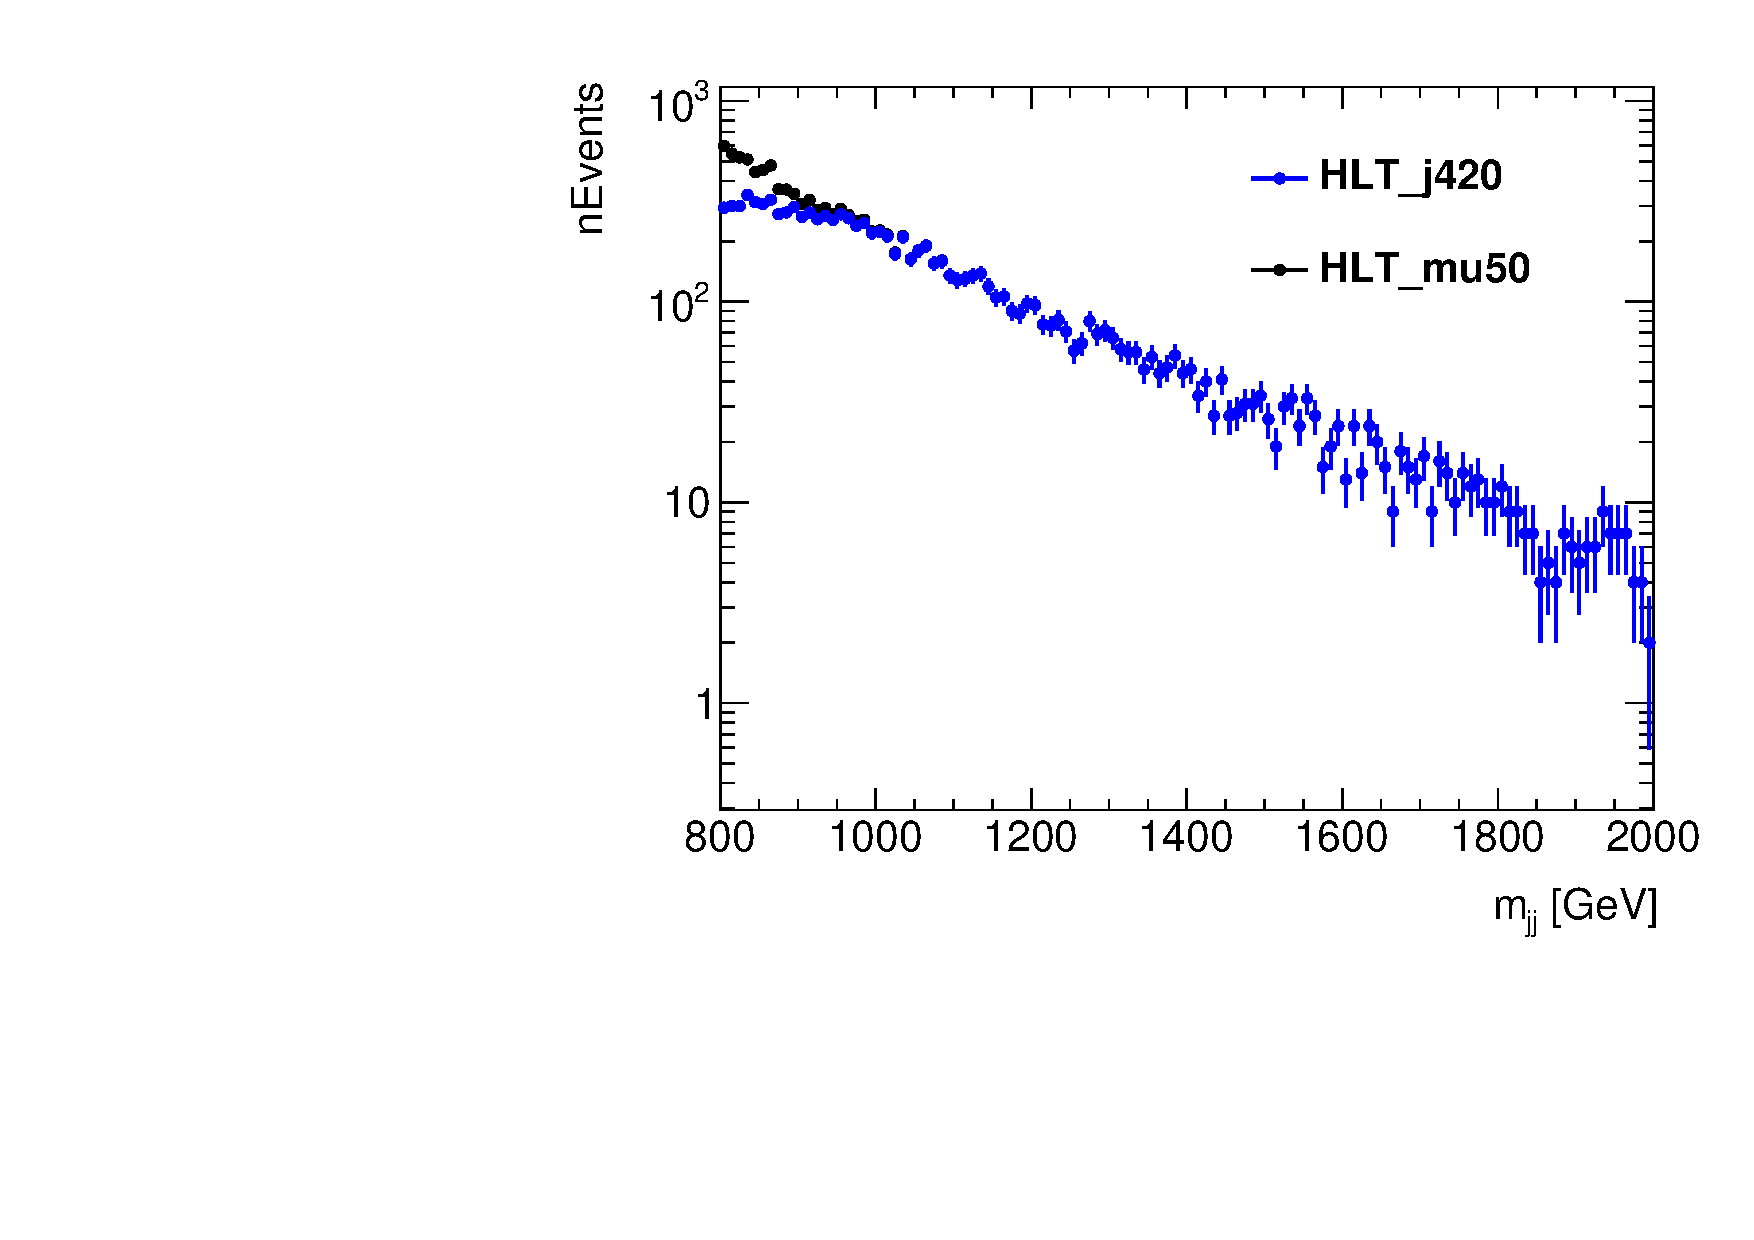
\includegraphics[width=0.48\columnwidth]{figures/massturnon/app_triggerturnon/mjj_qg_turnon_yStar0p6_Data15}}
        \subfigure[2 g-tag]{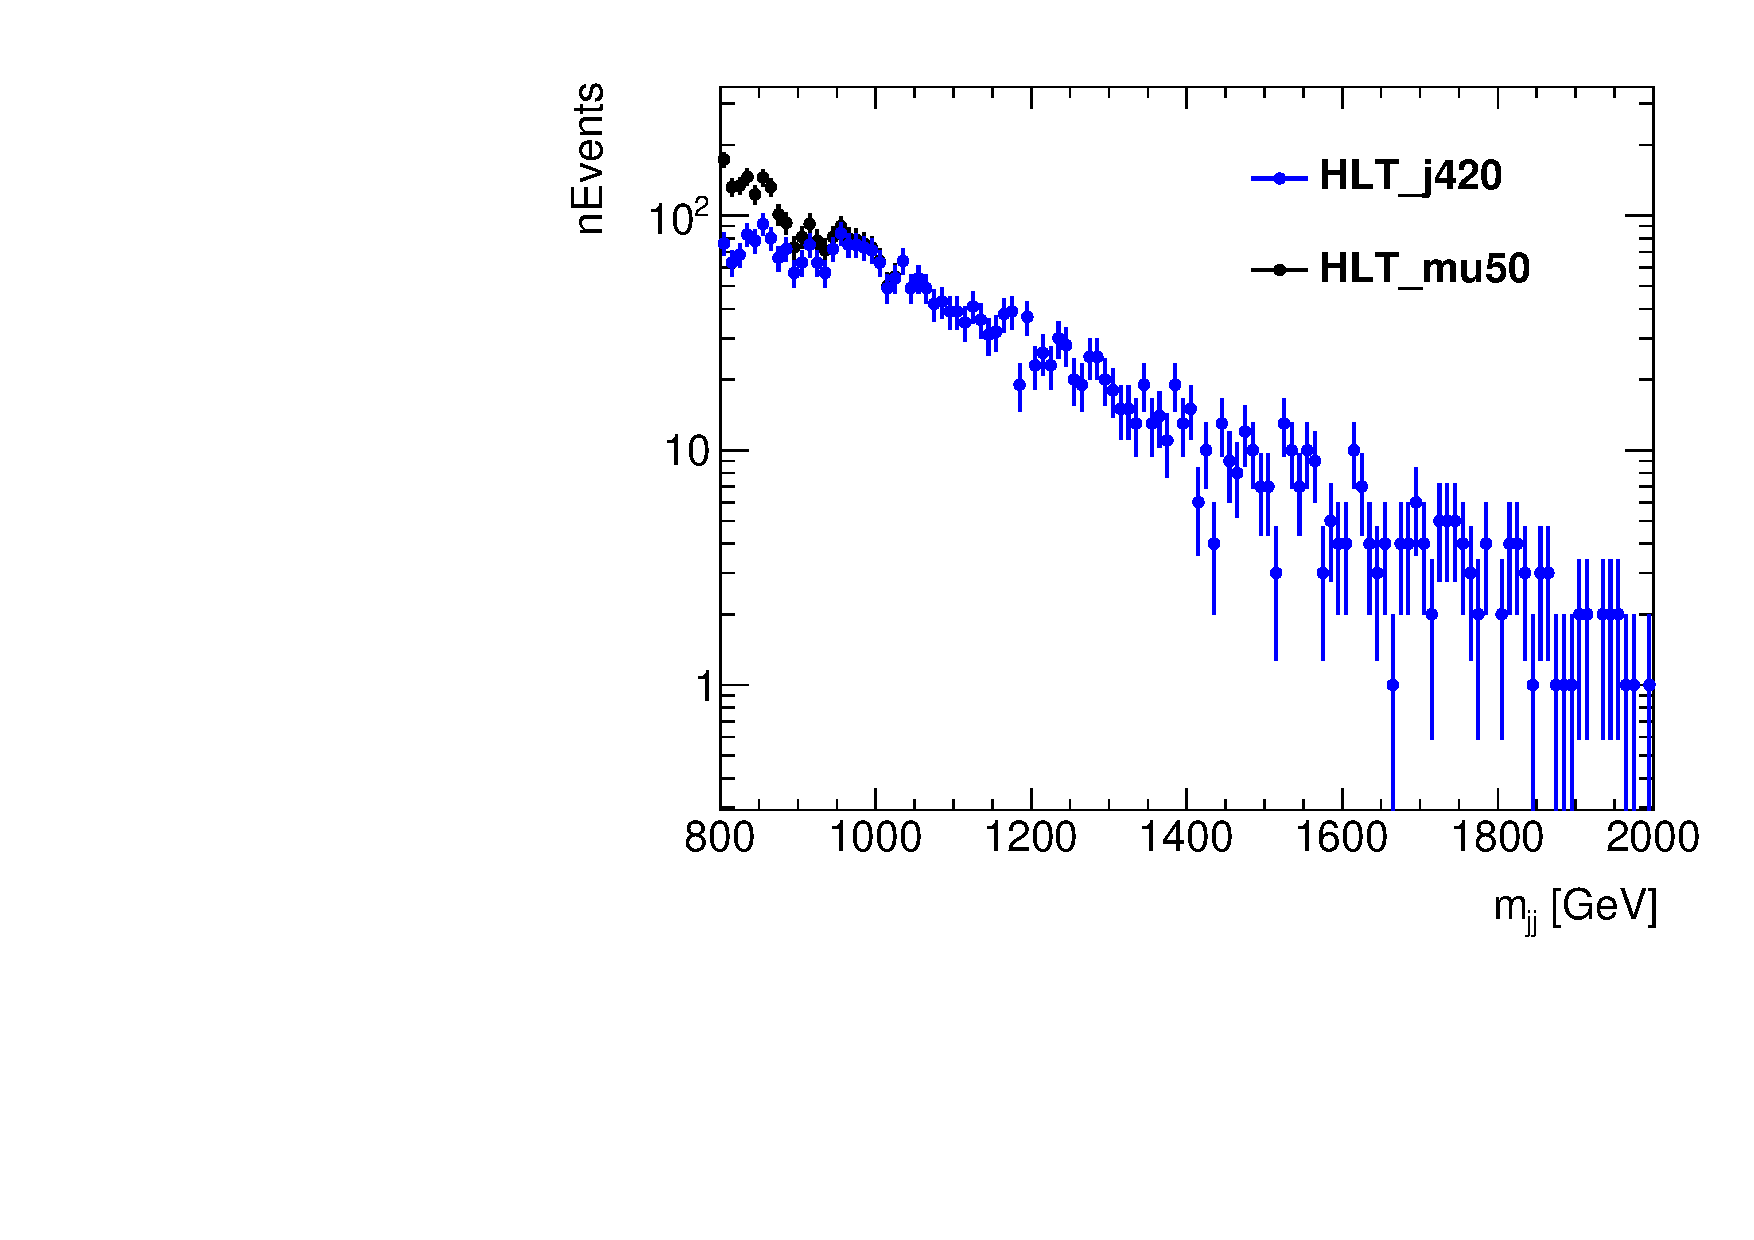
\includegraphics[width=0.48\columnwidth]{figures/massturnon/app_triggerturnon/mjj_gg_turnon_yStar0p6_Data15}}
        \\
        \subfigure[$\geq$1 g-tag]{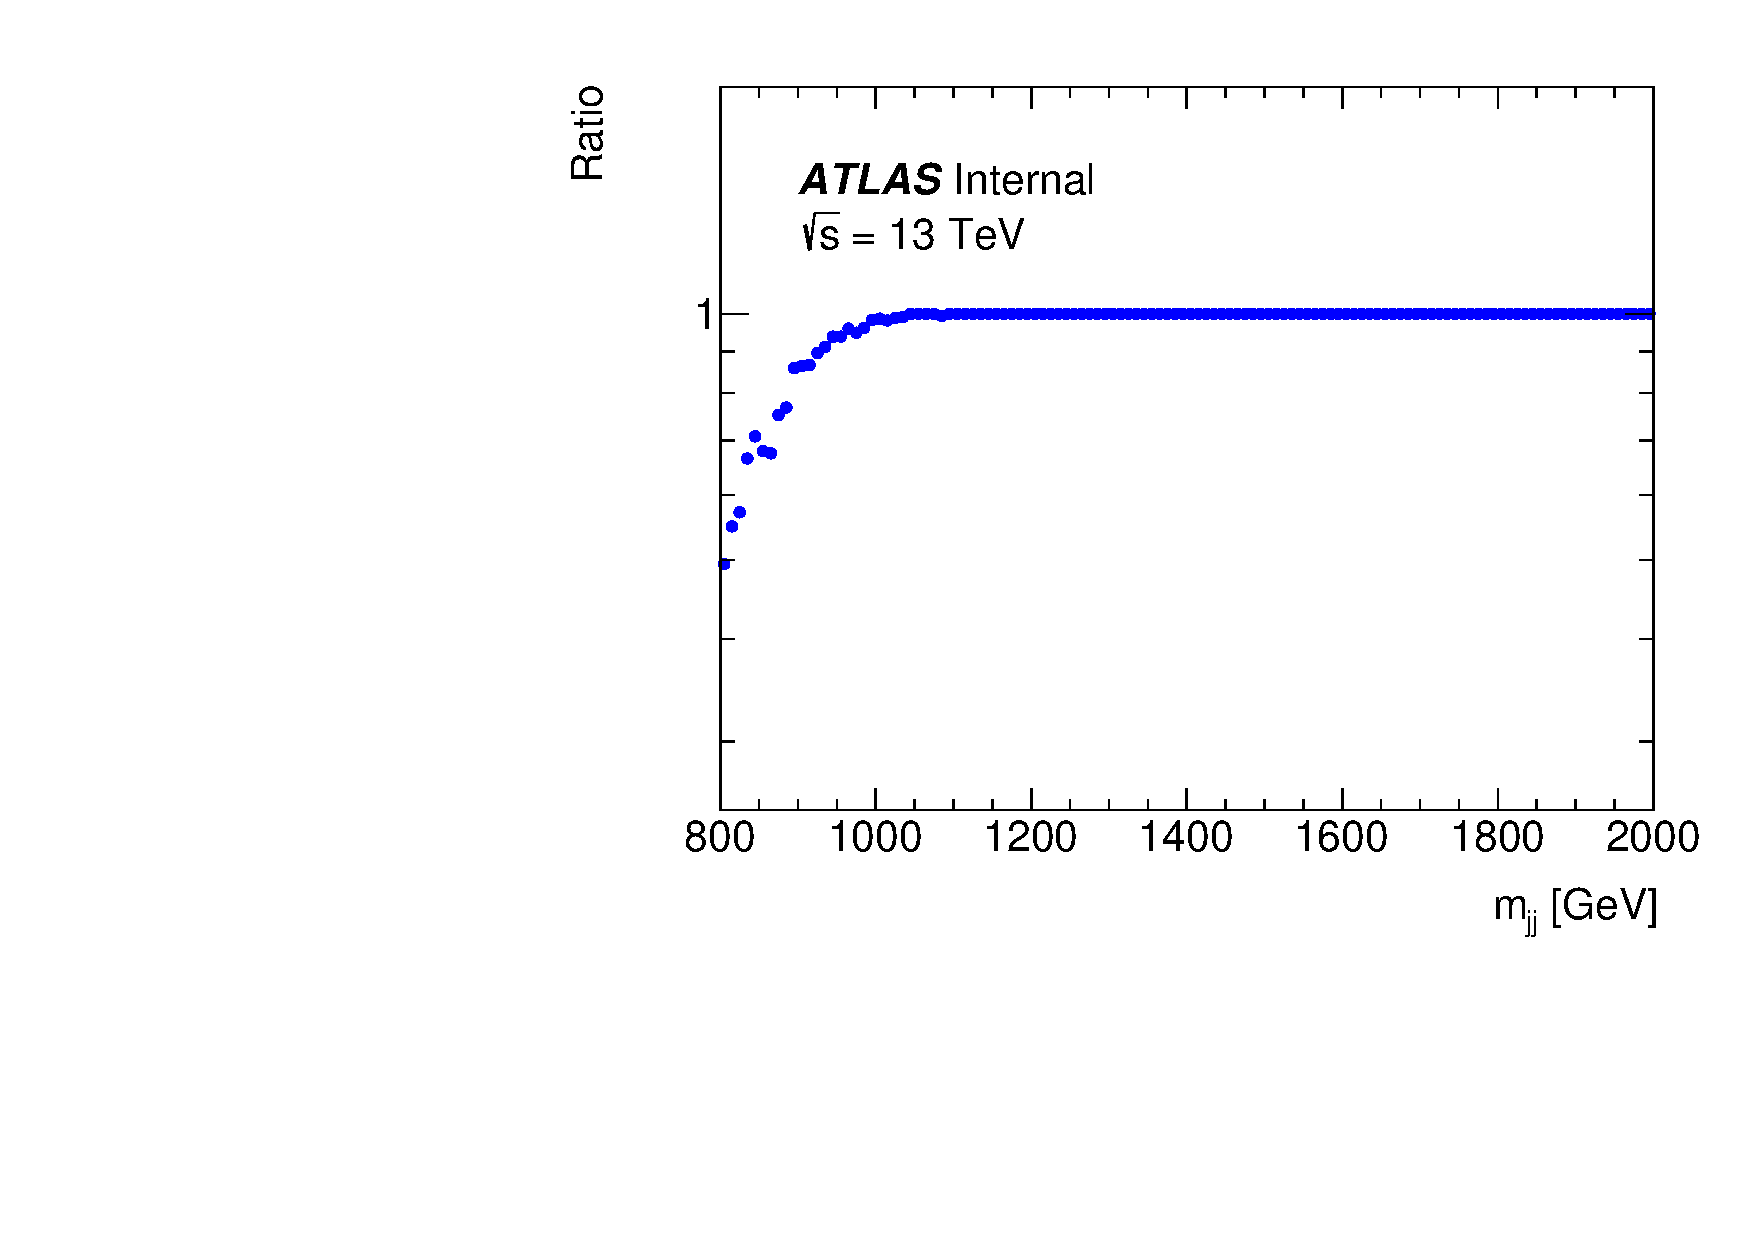
\includegraphics[width=0.48\columnwidth]{figures/massturnon/app_triggerturnon/Ratio_mjj_qg_turnon_yStar0p6_Data15}}
        \subfigure[2 g-tag]{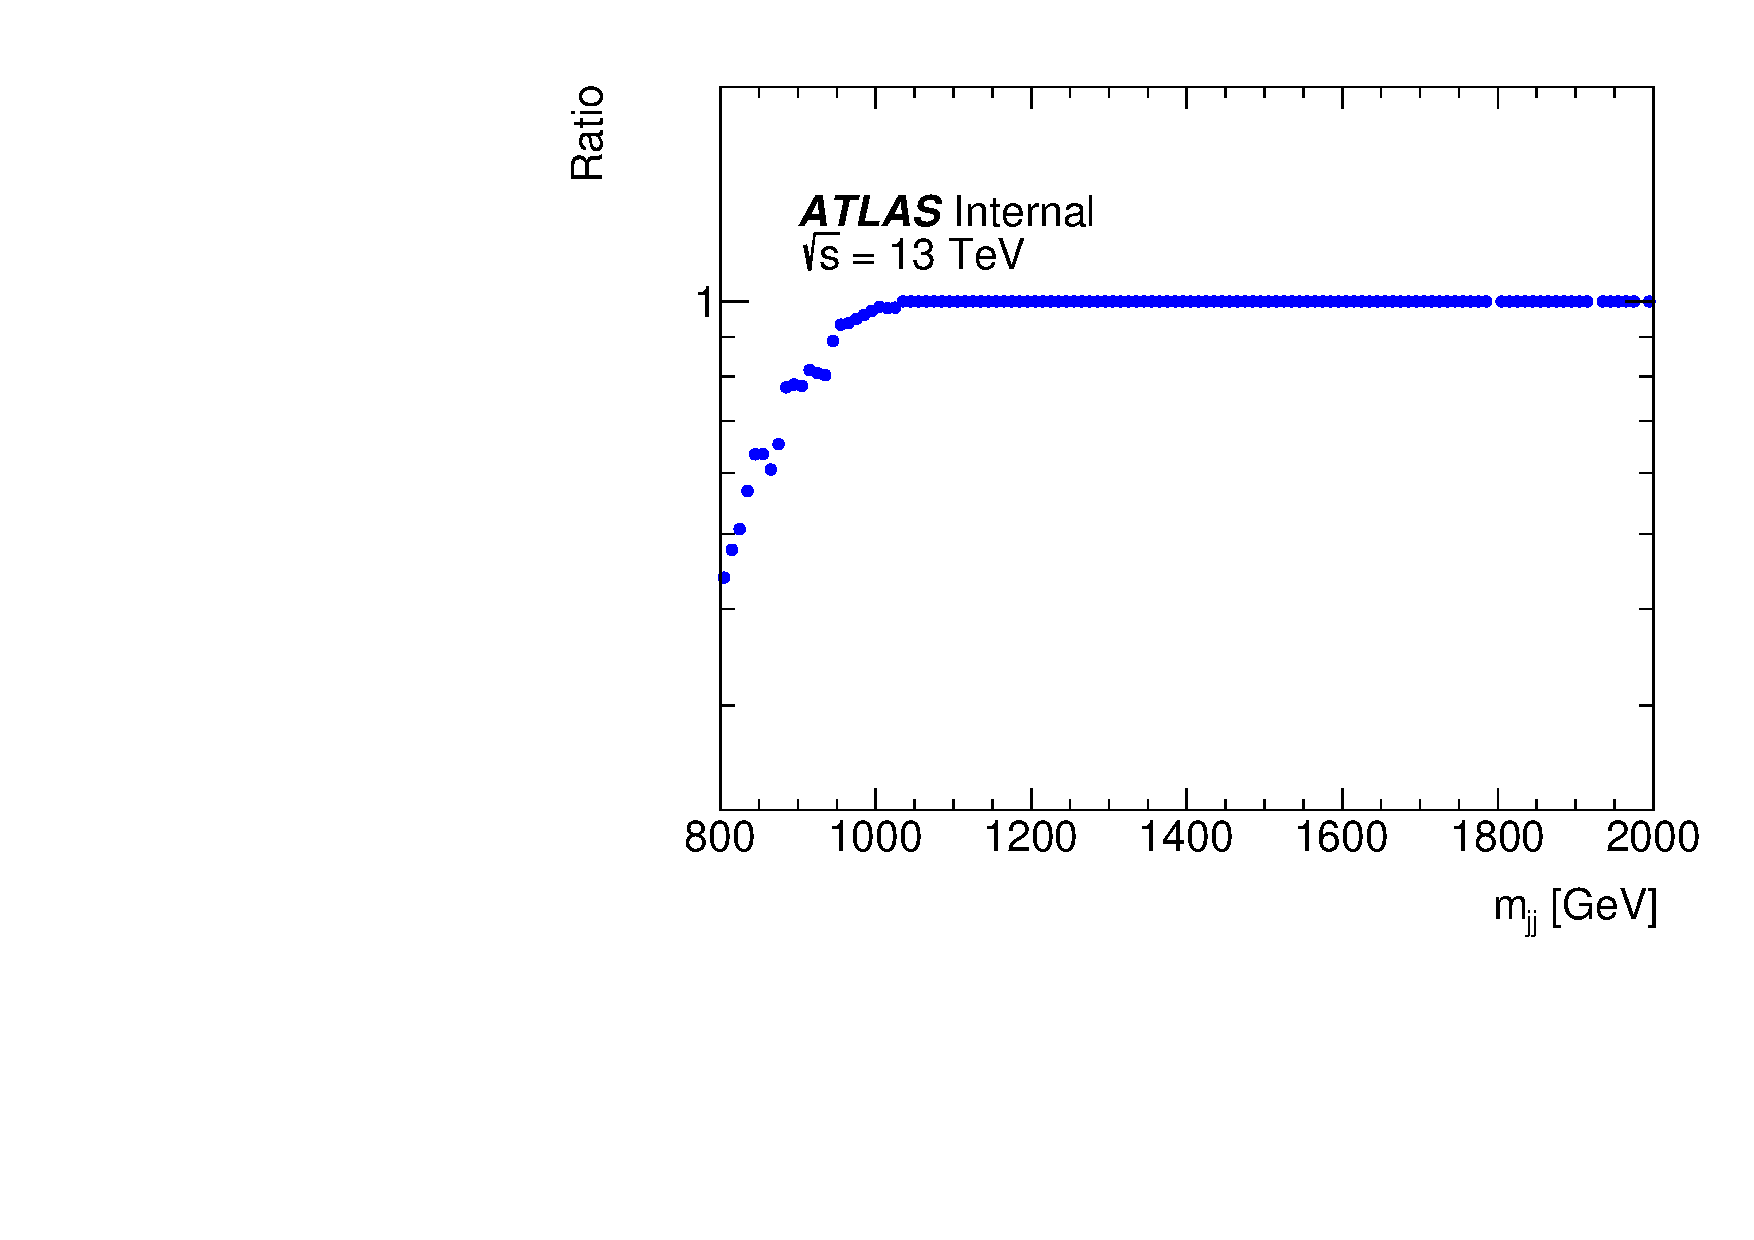
\includegraphics[width=0.48\columnwidth]{figures/massturnon/app_triggerturnon/Ratio_mjj_gg_turnon_yStar0p6_Data15}}

        \caption{Efficiencies as a function of \mjj\ for $|\ystar|<0.6$ using HLT\_j420 compared with HLT\_mu50 in the case of comparison of mass spectra with
        (a) $\geq$1 g-tag, (b) 2 g-tag and the ratio between the two (c) $\geq$1 g-tag and (d) 2 g-tag for 2015 data.}
        \label{fig:trigger-yStar0p6-Data15}
\end{figure}

\begin{figure}[htbp]
        \centering
        \subfigure[$\geq$1 g-tag]{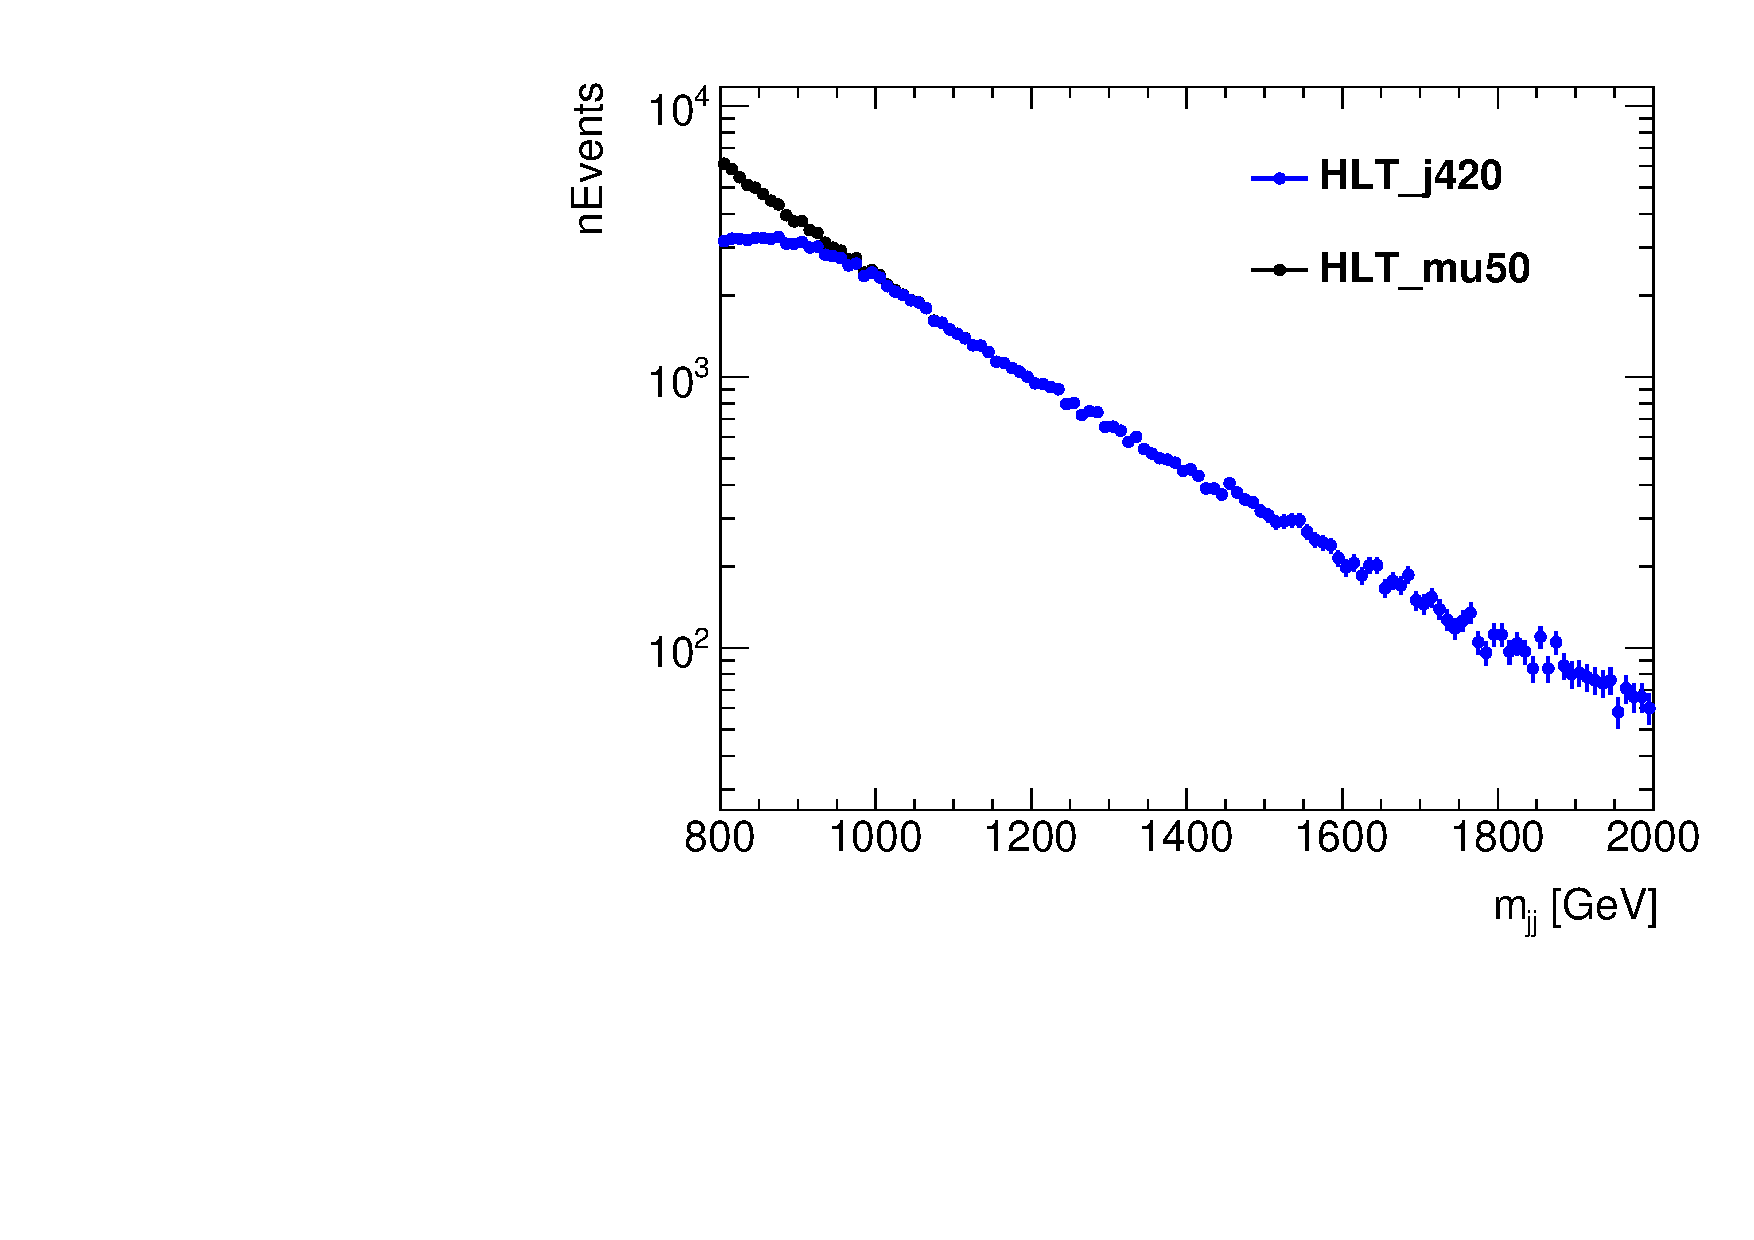
\includegraphics[width=0.48\columnwidth]{figures/massturnon/app_triggerturnon/mjj_qg_turnon_yStar0p6_Data16}}
        \subfigure[2 g-tag]{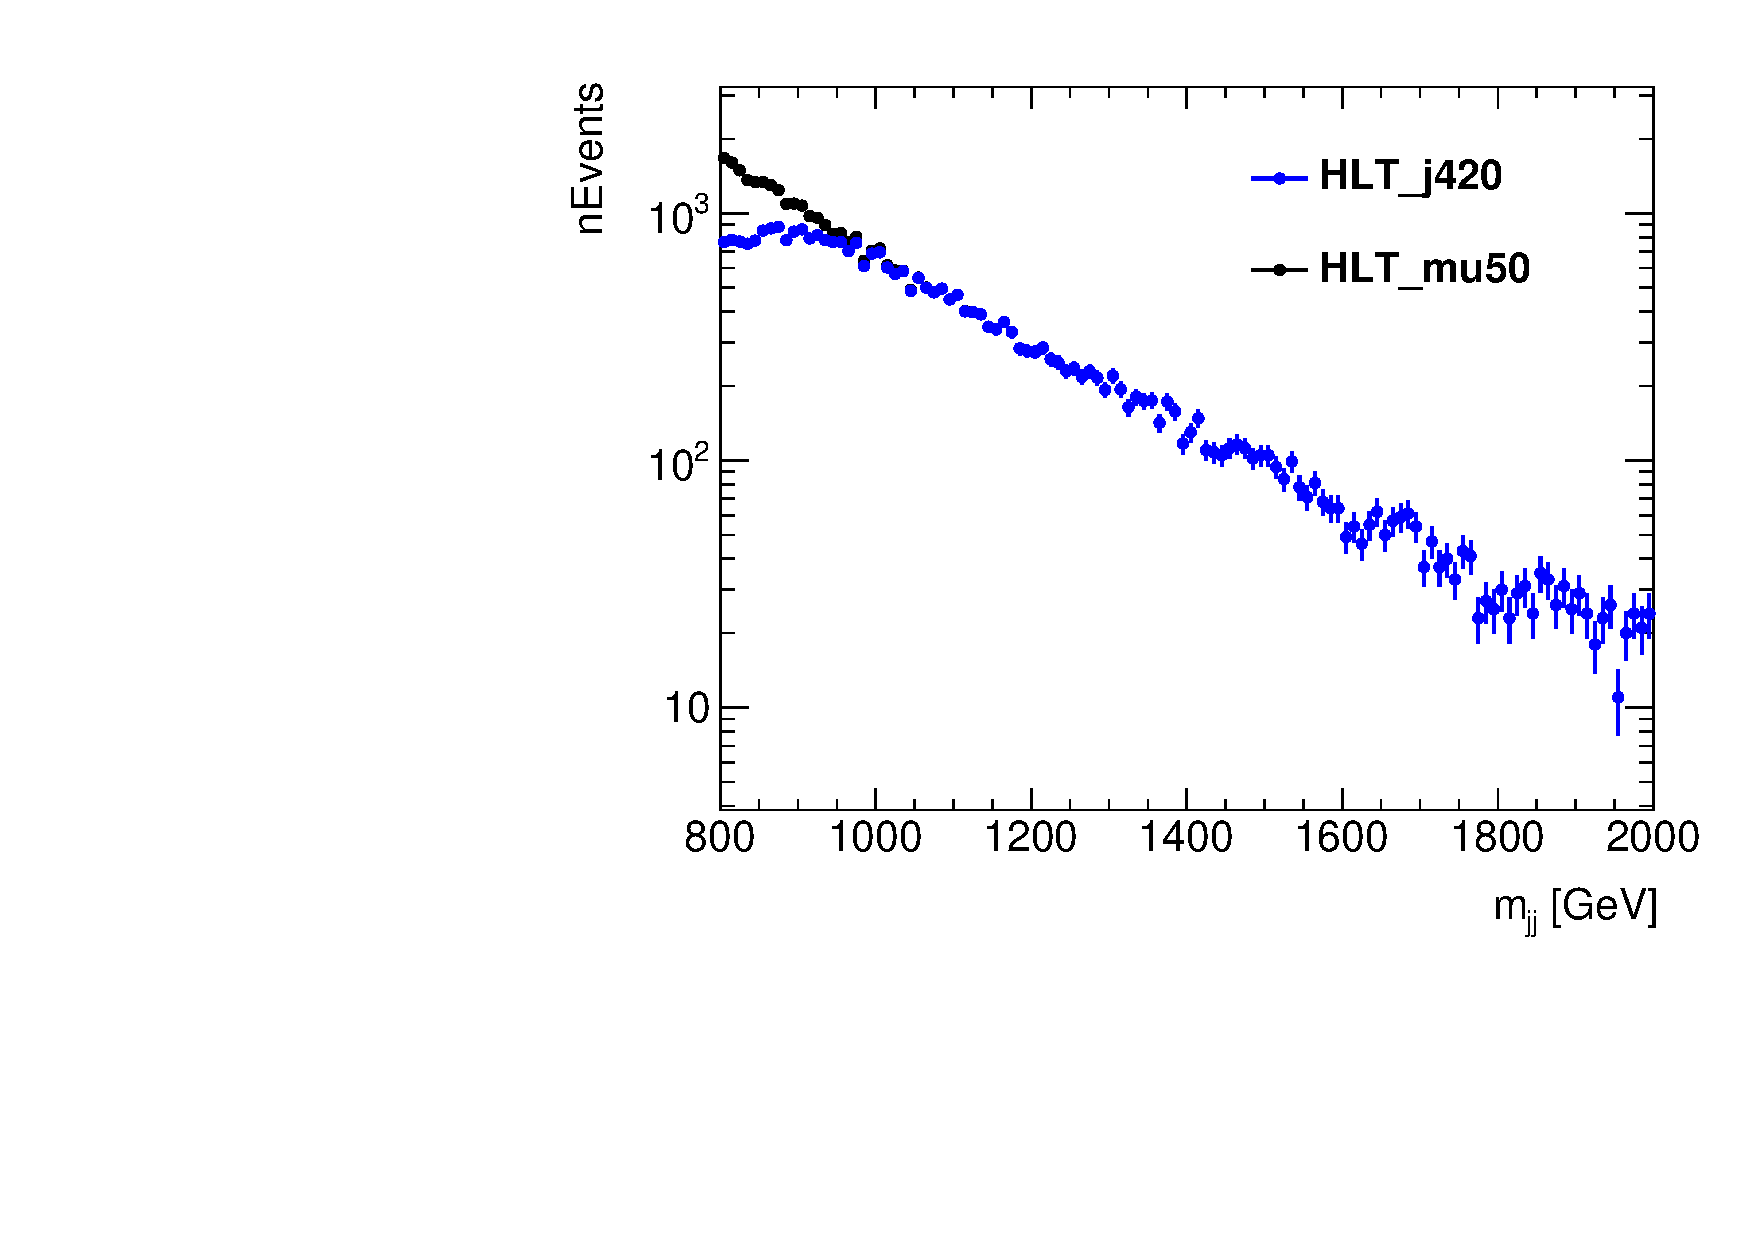
\includegraphics[width=0.48\columnwidth]{figures/massturnon/app_triggerturnon/mjj_gg_turnon_yStar0p6_Data16}}
        \\
        \subfigure[$\geq$1 g-tag]{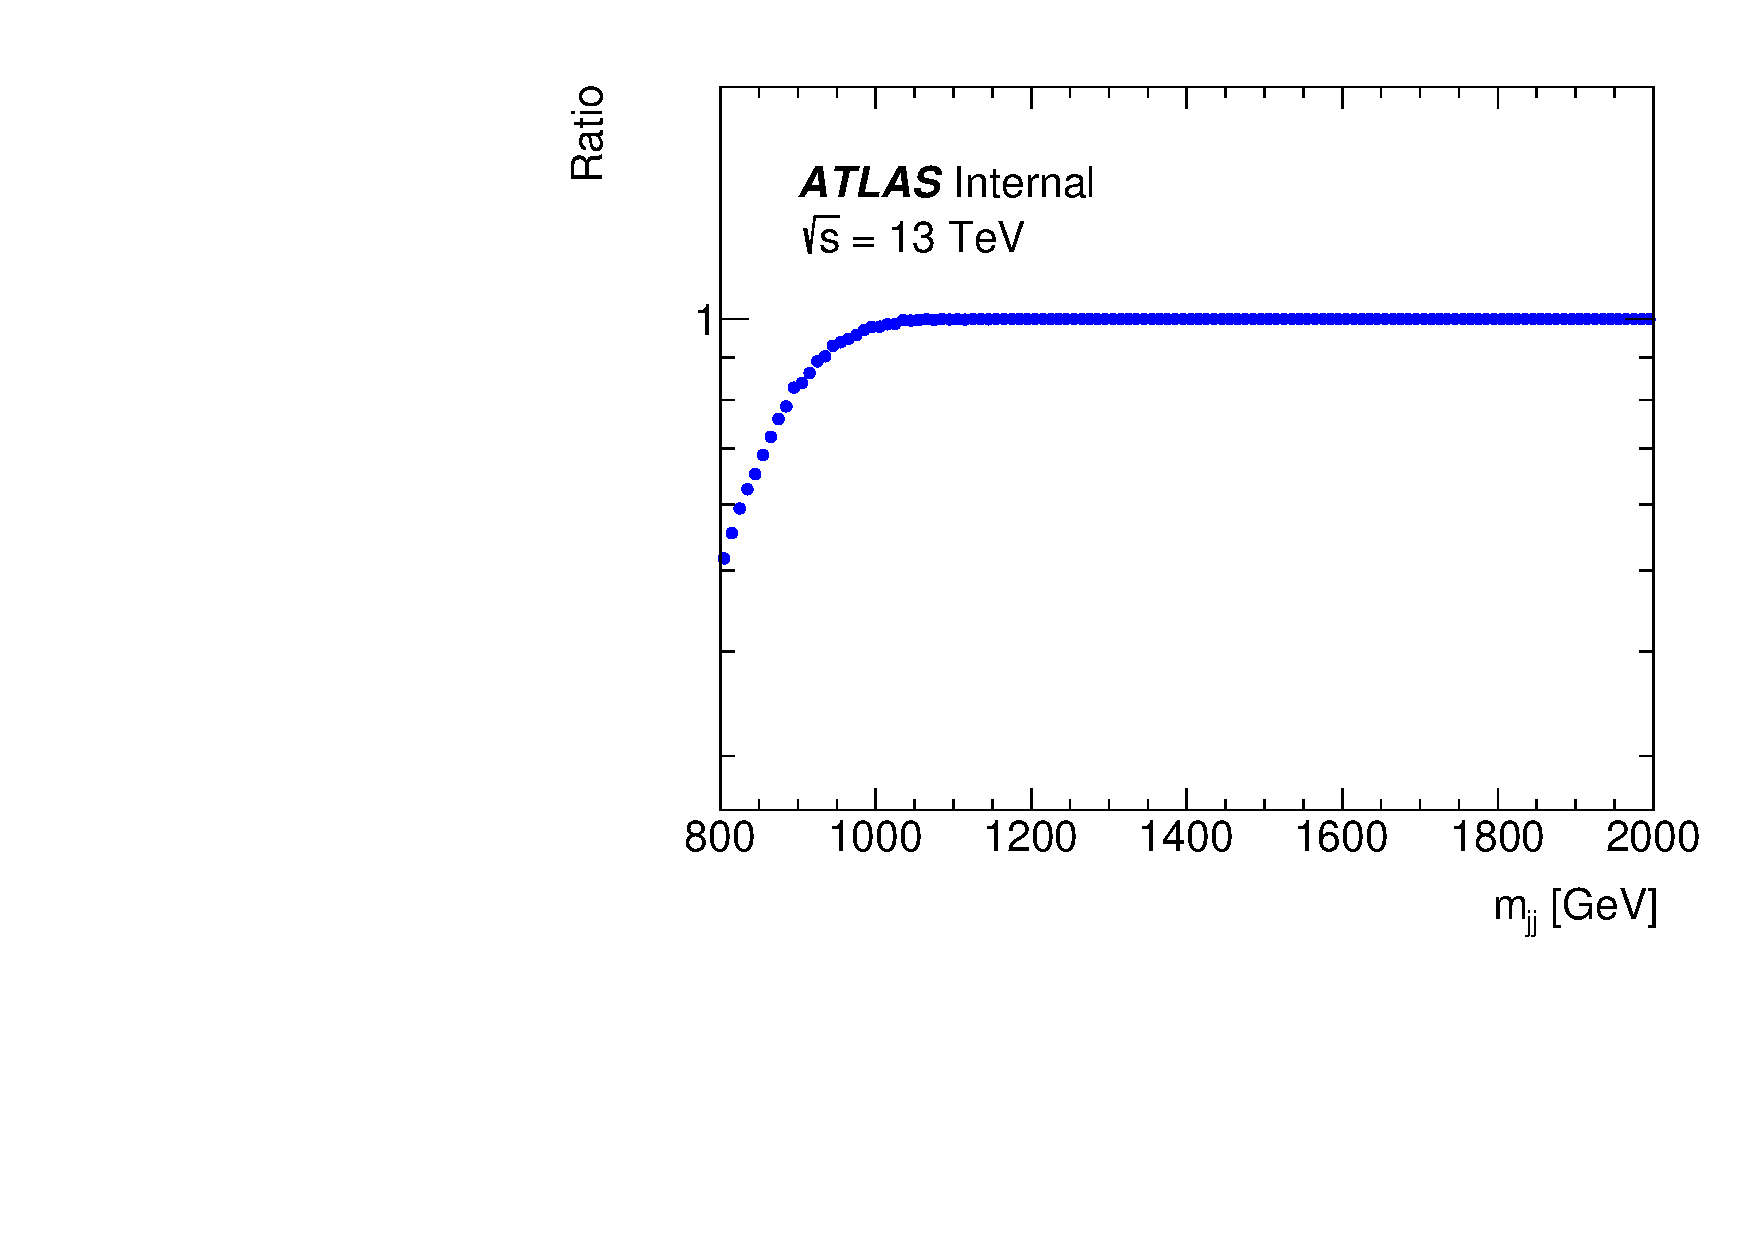
\includegraphics[width=0.48\columnwidth]{figures/massturnon/app_triggerturnon/Ratio_mjj_qg_turnon_yStar0p6_Data16}}
        \subfigure[2 g-tag]{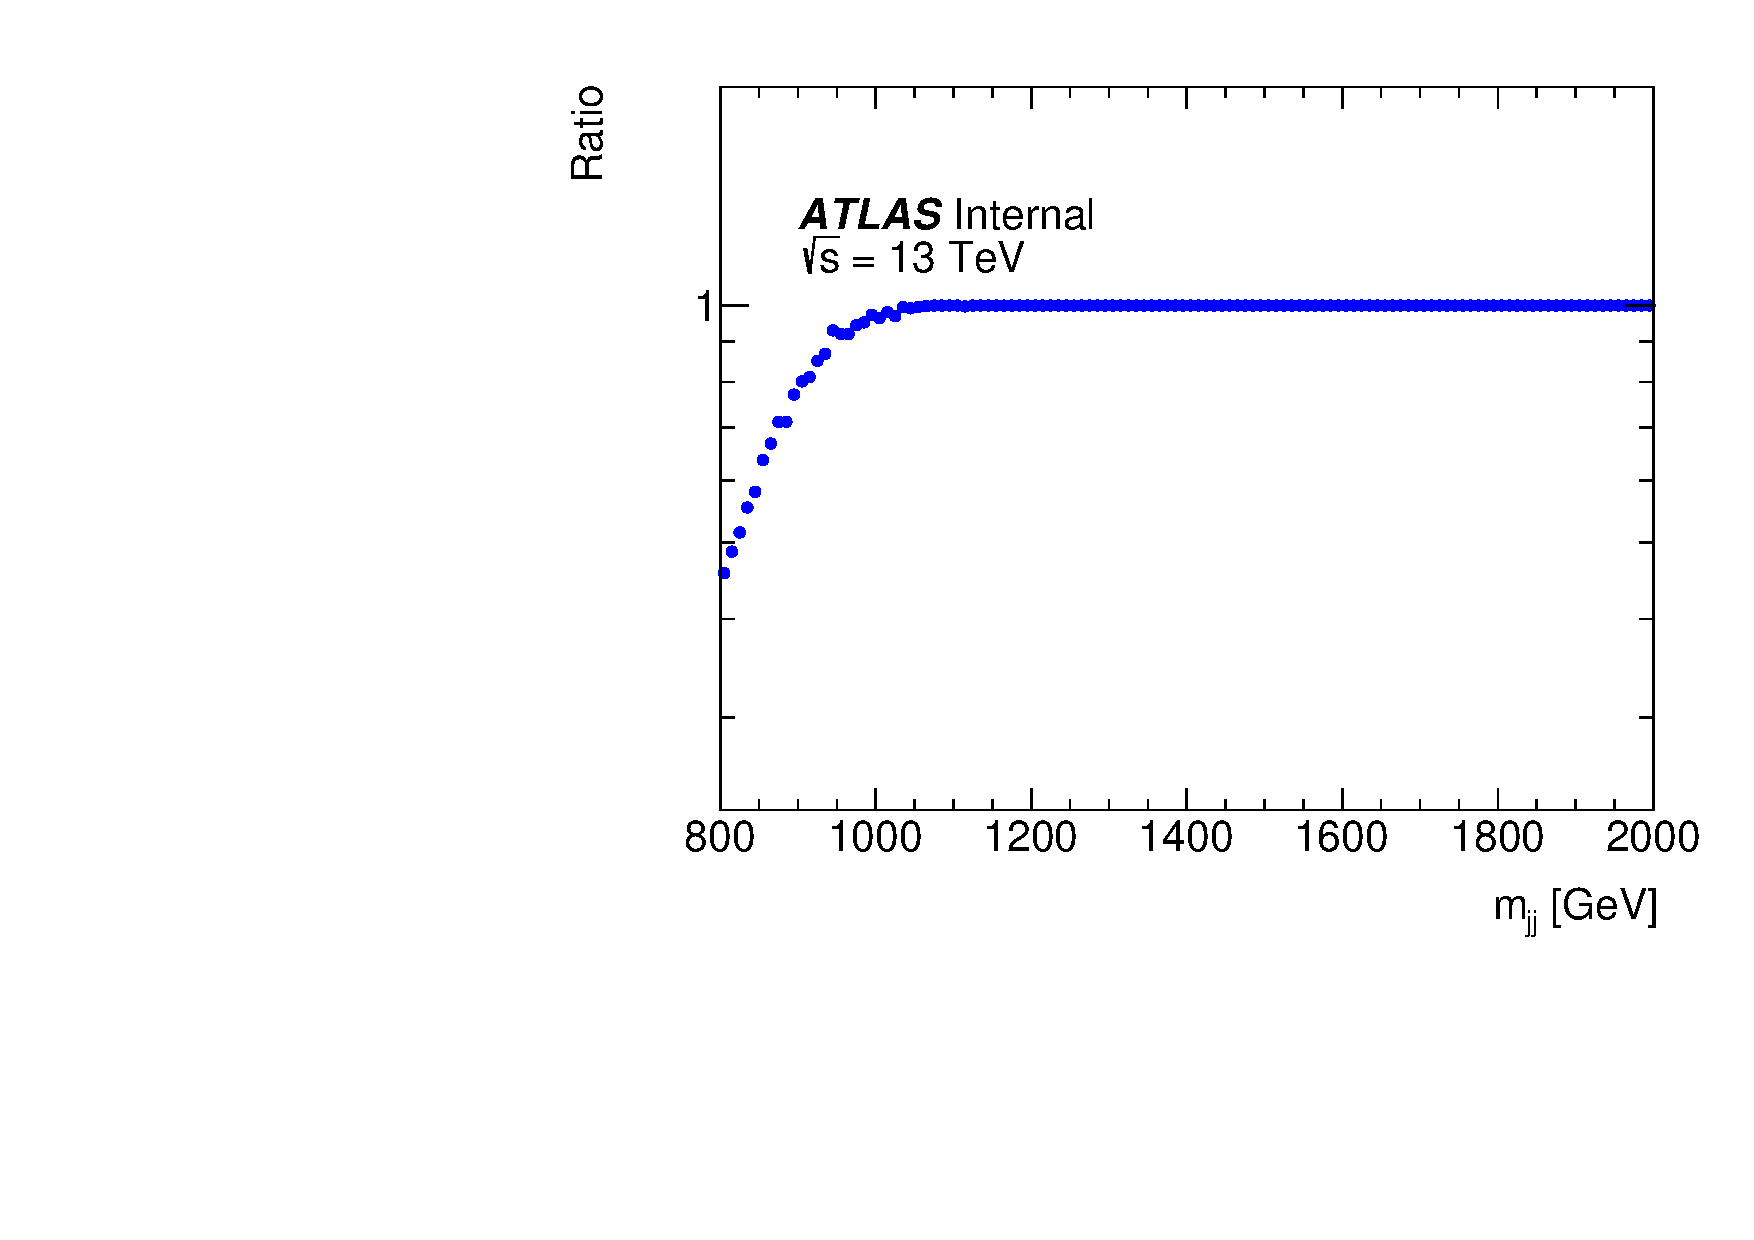
\includegraphics[width=0.48\columnwidth]{figures/massturnon/app_triggerturnon/Ratio_mjj_gg_turnon_yStar0p6_Data16}}

        \caption{Efficiencies as a function of \mjj\ for $|\ystar|<0.6$ using HLT\_j420 compared with HLT\_mu50 in the case of comparison of mass spectra with
        (a) $\geq$1 g-tag, (b) 2 g-tag and the ratio between the two (c) $\geq$1 g-tag and (d) 2 g-tag for 2016 data.}
\end{figure}

\begin{figure}[htbp]
        \centering
        \subfigure[$\geq$1 g-tag]{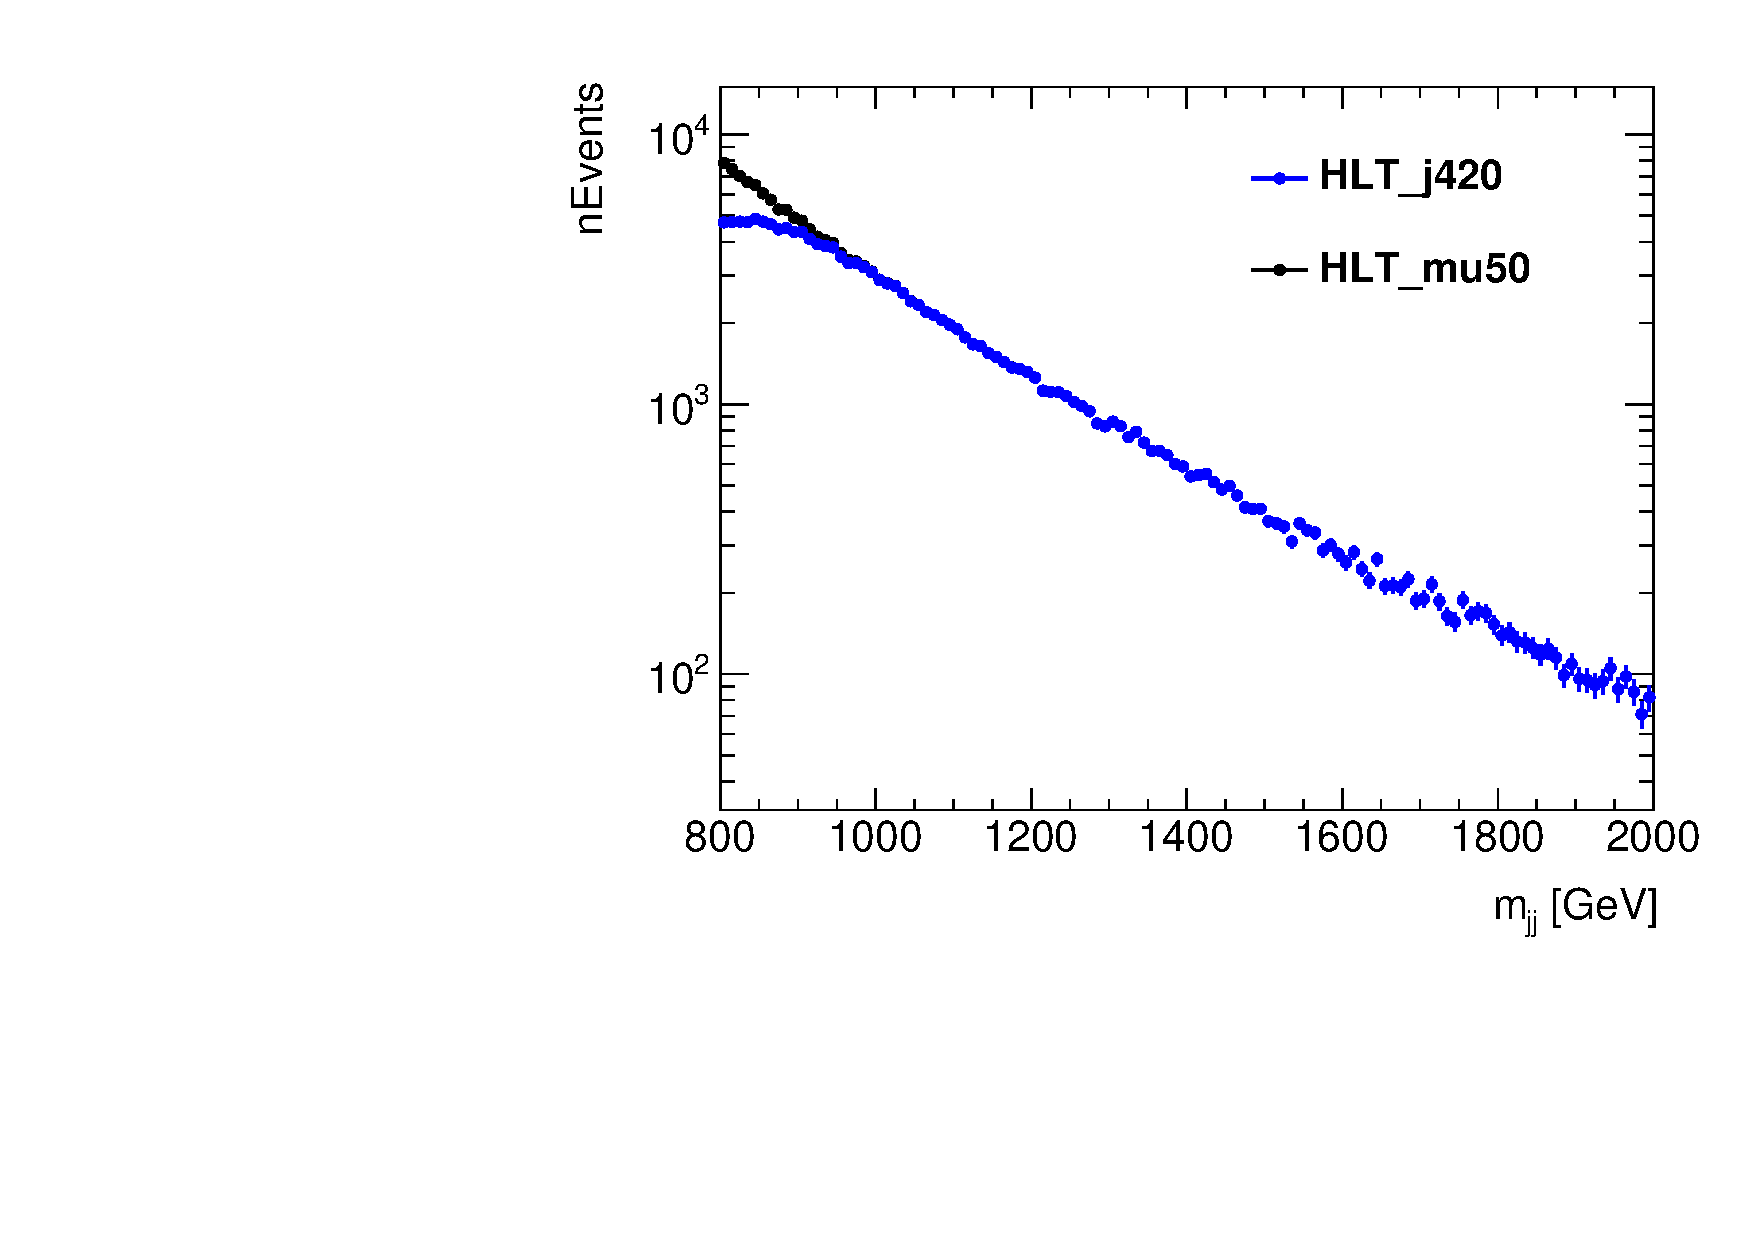
\includegraphics[width=0.48\columnwidth]{figures/massturnon/app_triggerturnon/mjj_qg_turnon_yStar0p6_Data17}}
        \subfigure[2 g-tag]{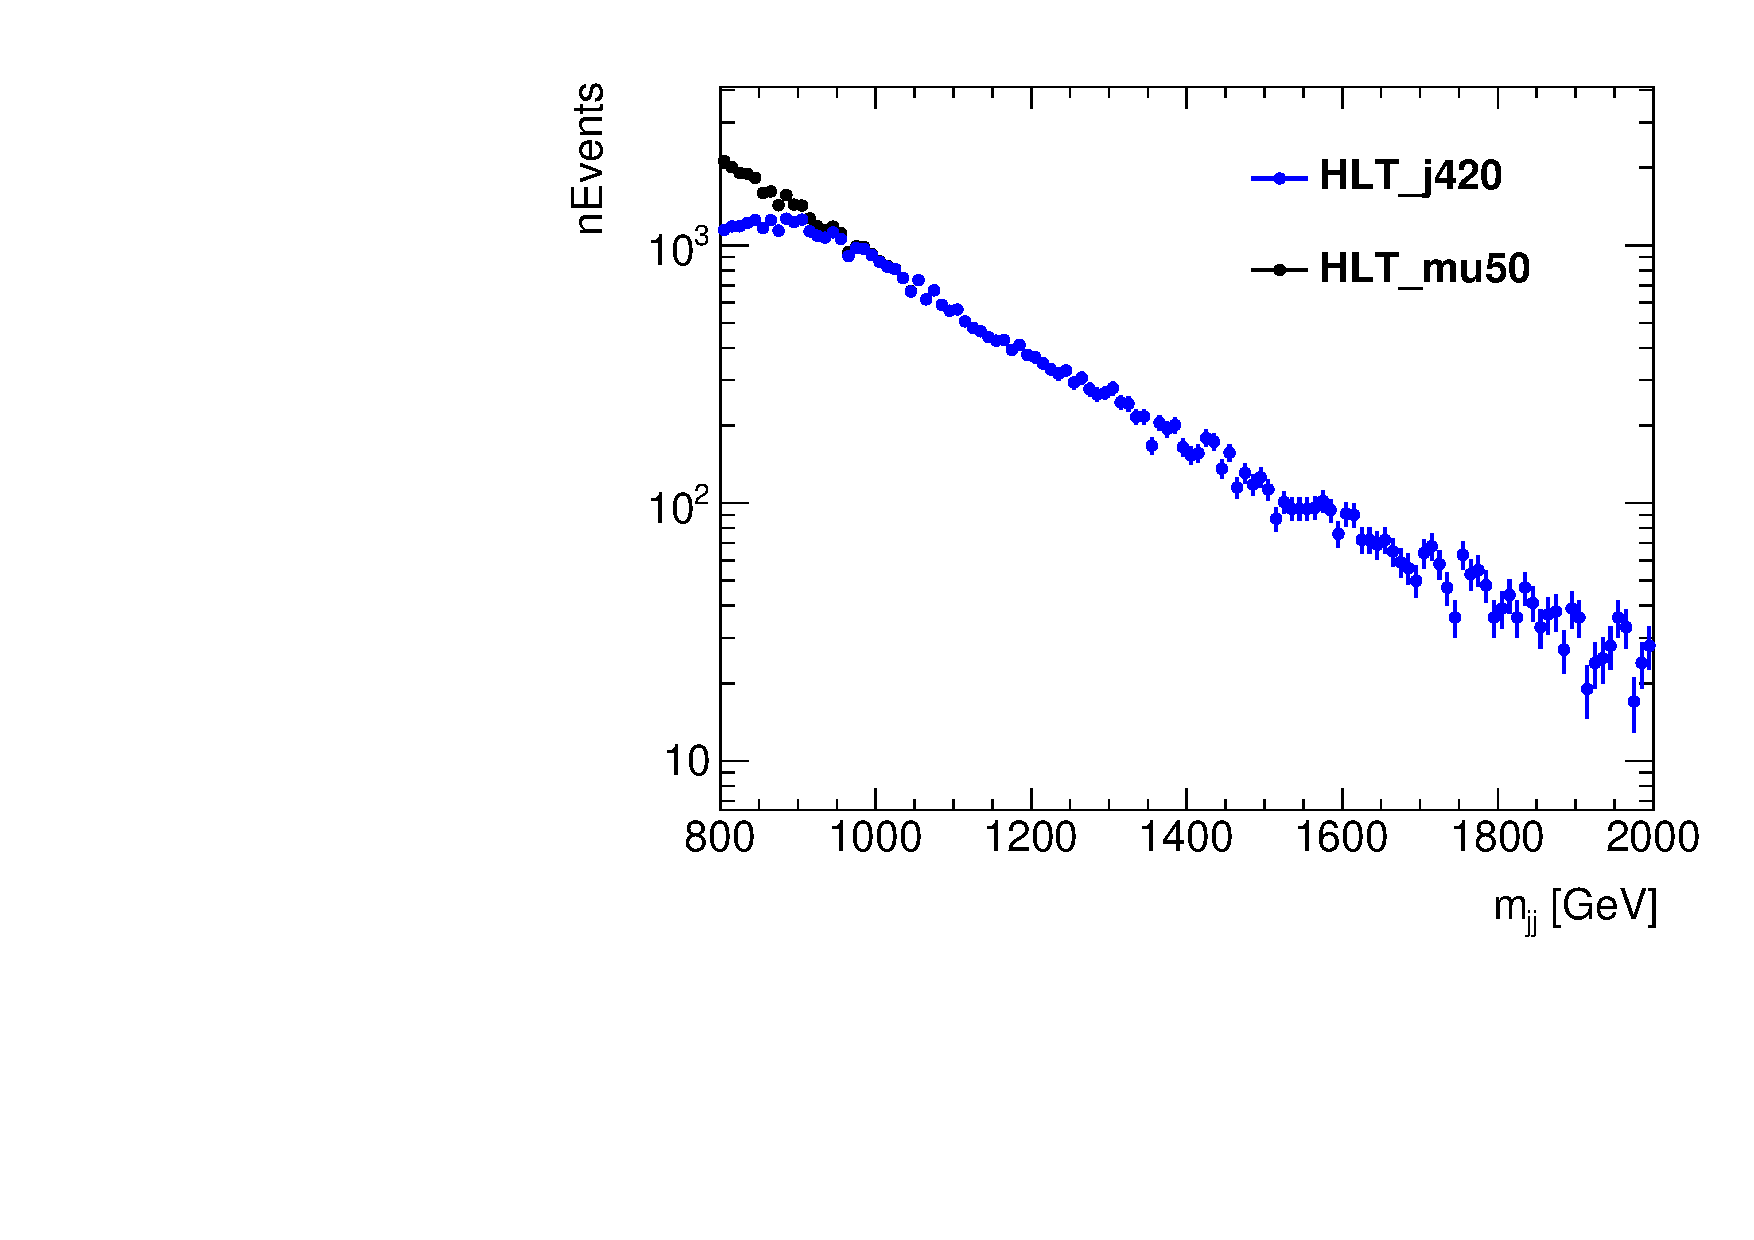
\includegraphics[width=0.48\columnwidth]{figures/massturnon/app_triggerturnon/mjj_gg_turnon_yStar0p6_Data17}}
        \\
        \subfigure[$\geq$1 g-tag]{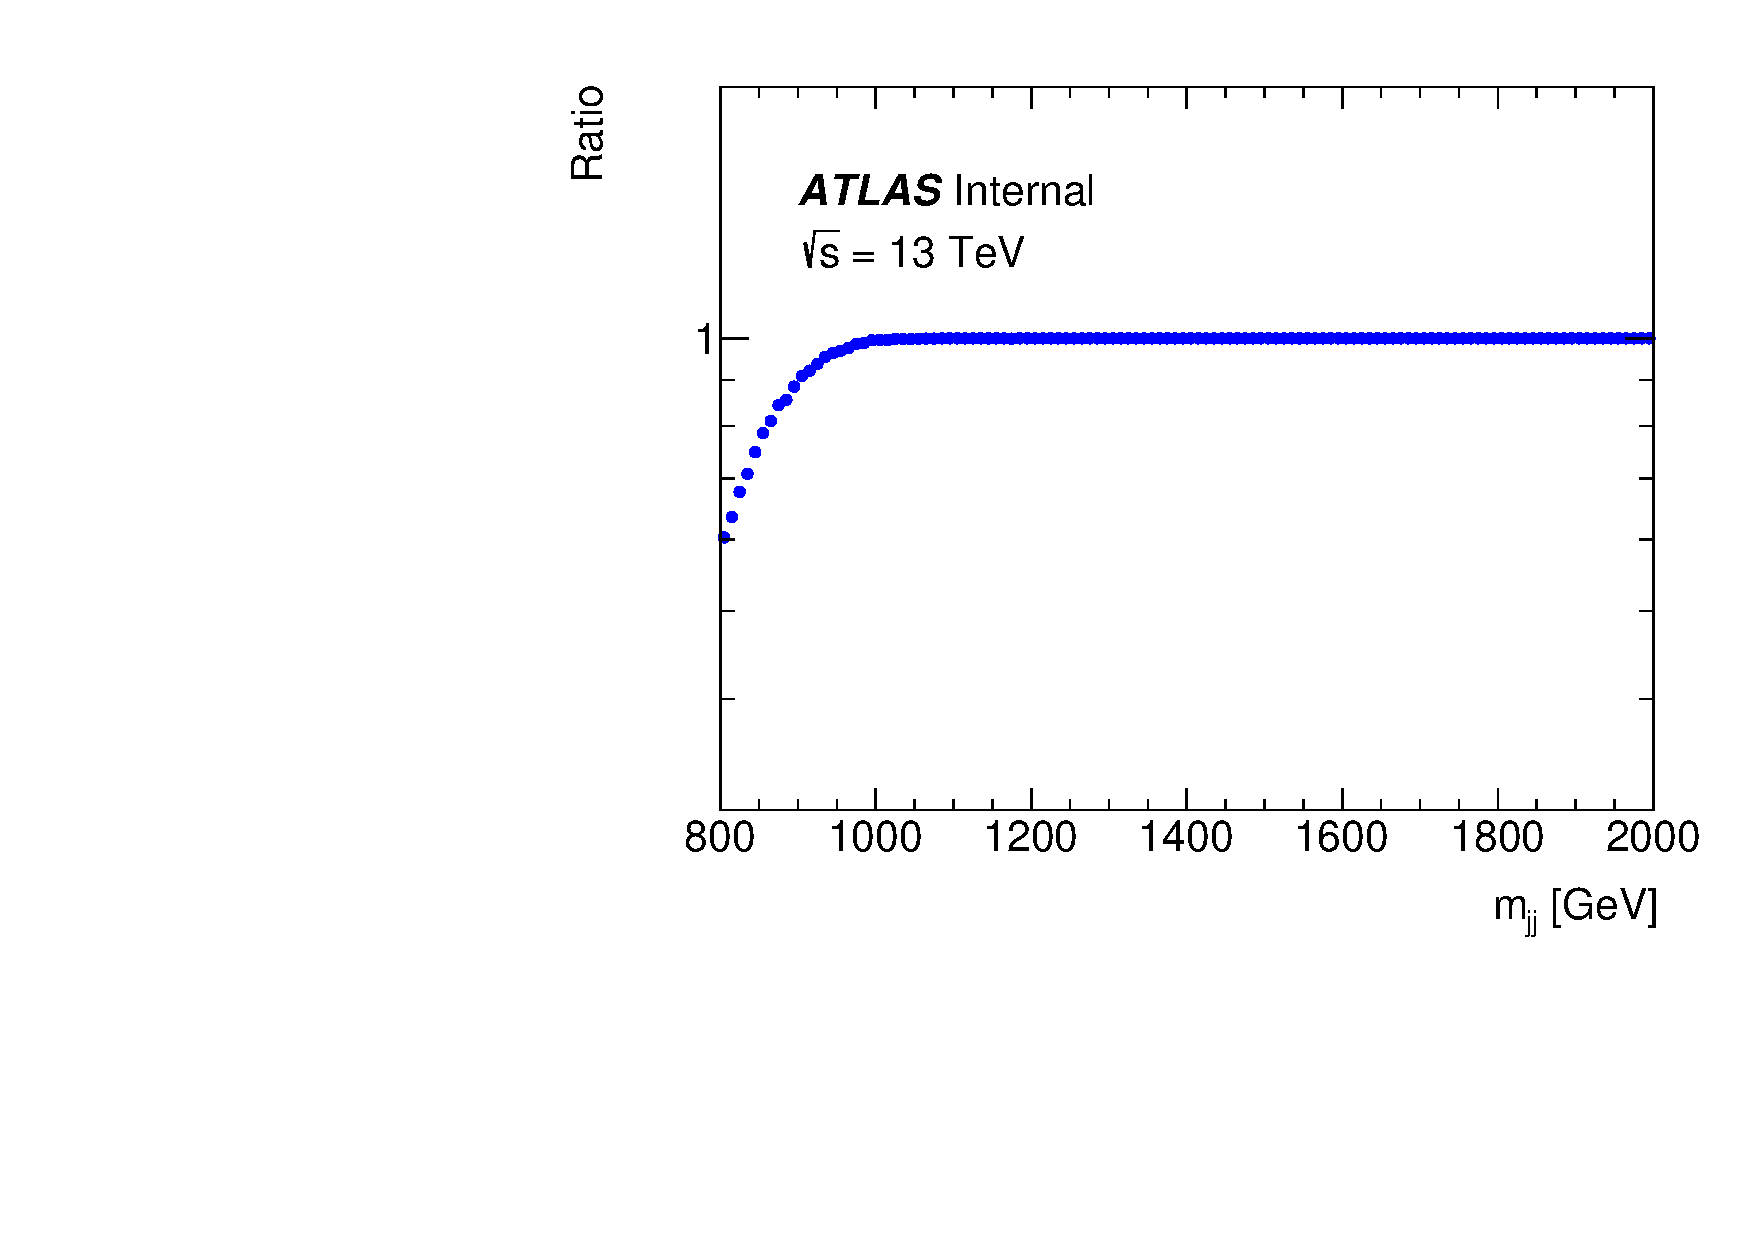
\includegraphics[width=0.48\columnwidth]{figures/massturnon/app_triggerturnon/Ratio_mjj_qg_turnon_yStar0p6_Data17}}
        \subfigure[2 g-tag]{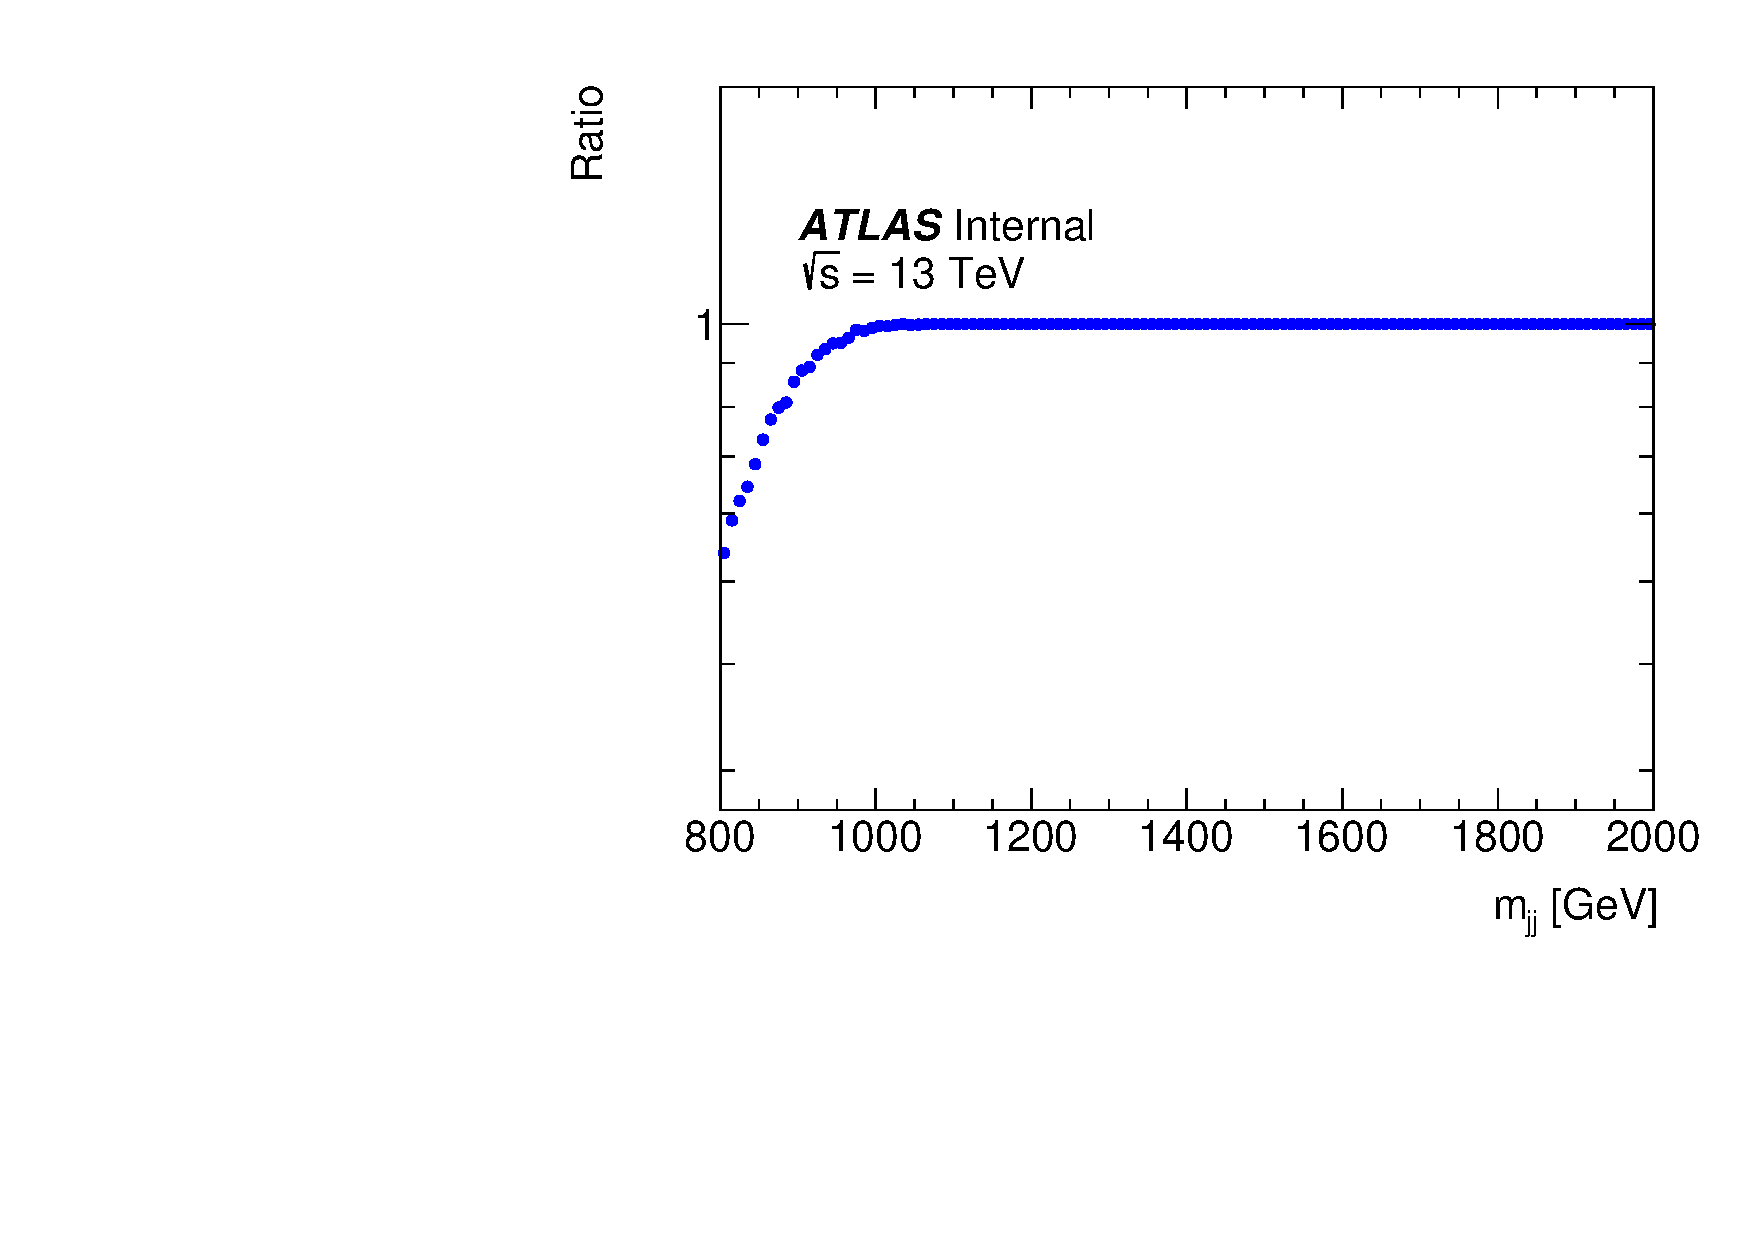
\includegraphics[width=0.48\columnwidth]{figures/massturnon/app_triggerturnon/Ratio_mjj_gg_turnon_yStar0p6_Data17}}

        \caption{Efficiencies as a function of \mjj\ for $|\ystar|<0.6$ using HLT\_j420 compared with HLT\_mu50 in the case of comparison of mass spectra with
        (a) $\geq$1 g-tag, (b) 2 g-tag and the ratio between the two (c) $\geq$1 g-tag and (d) 2 g-tag for 2017 data.}
\end{figure}

\begin{figure}[htbp]
        \centering
        \subfigure[$\geq$1 g-tag]{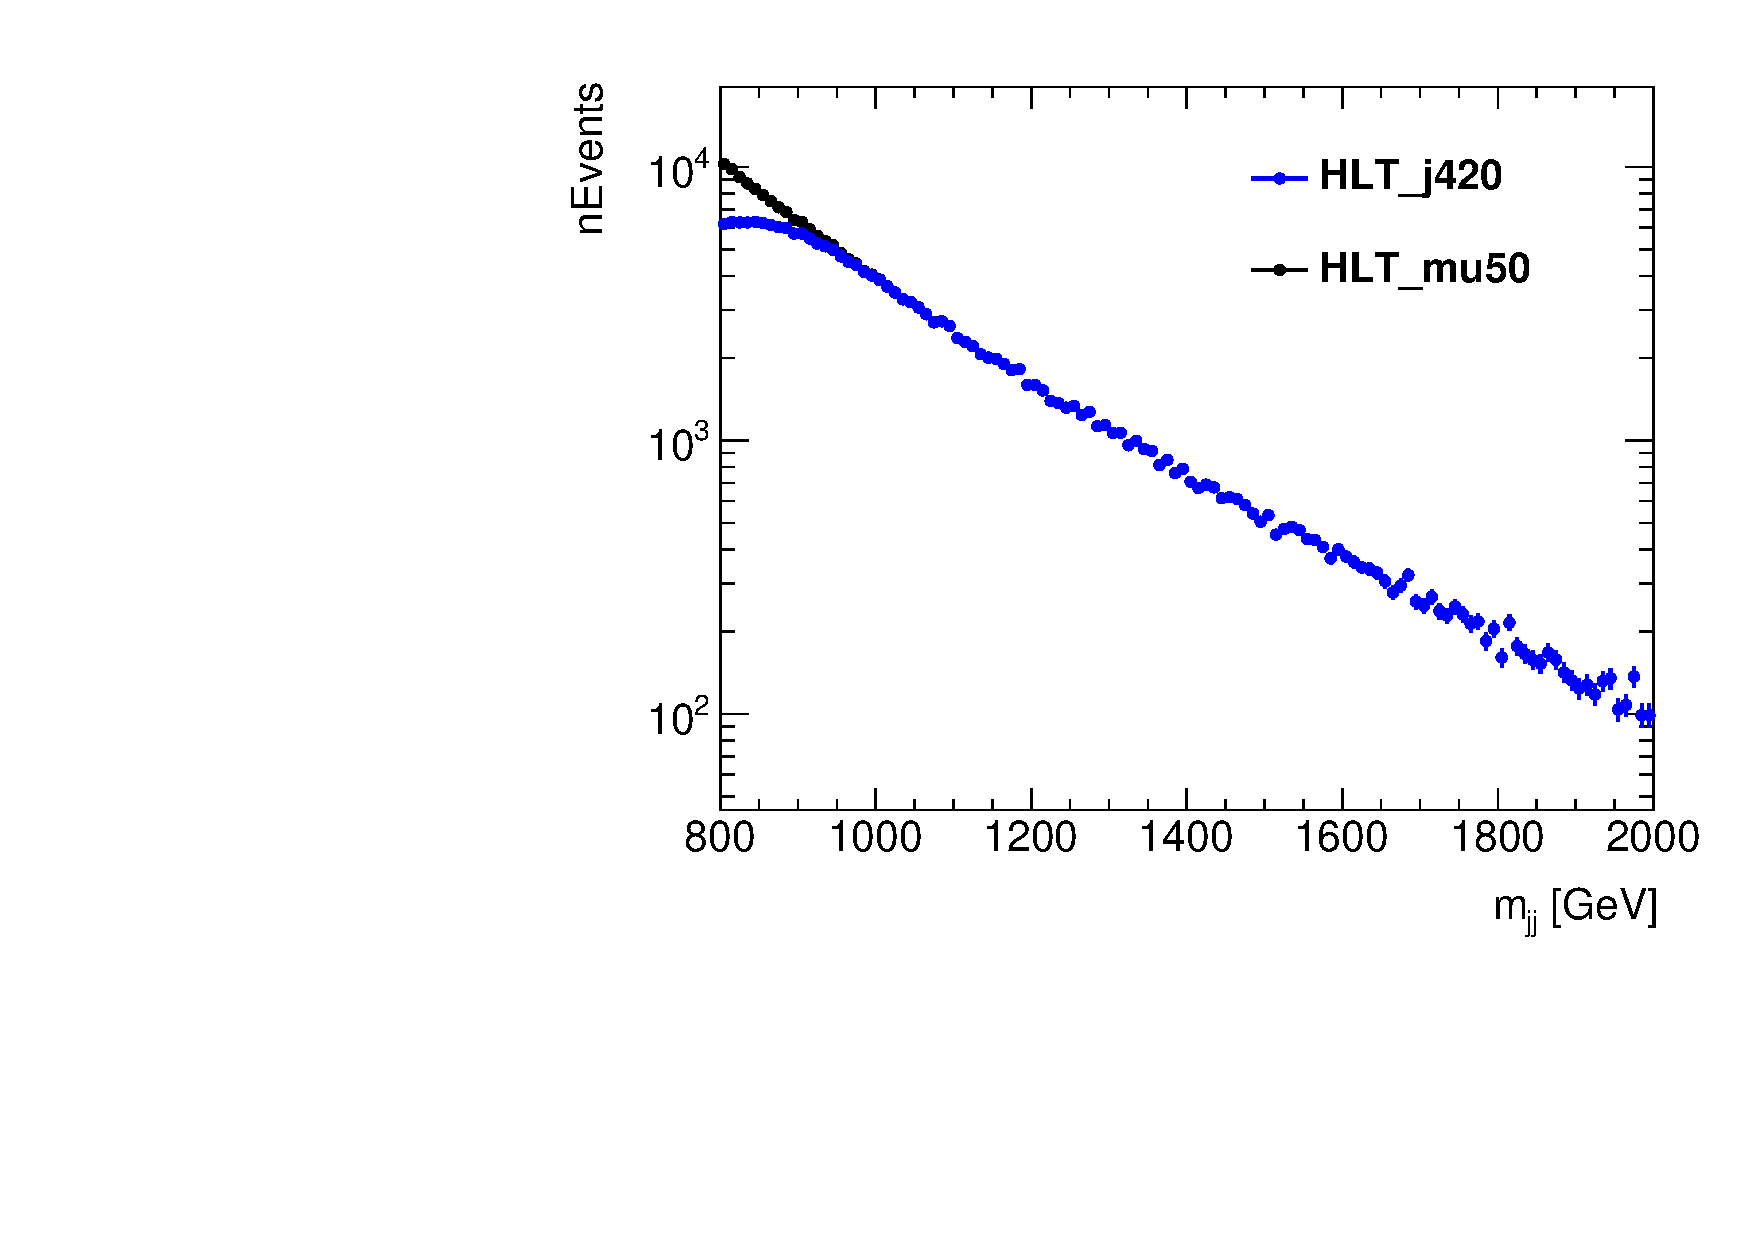
\includegraphics[width=0.48\columnwidth]{figures/massturnon/app_triggerturnon/mjj_qg_turnon_yStar0p6_Data18}}
        \subfigure[2 g-tag]{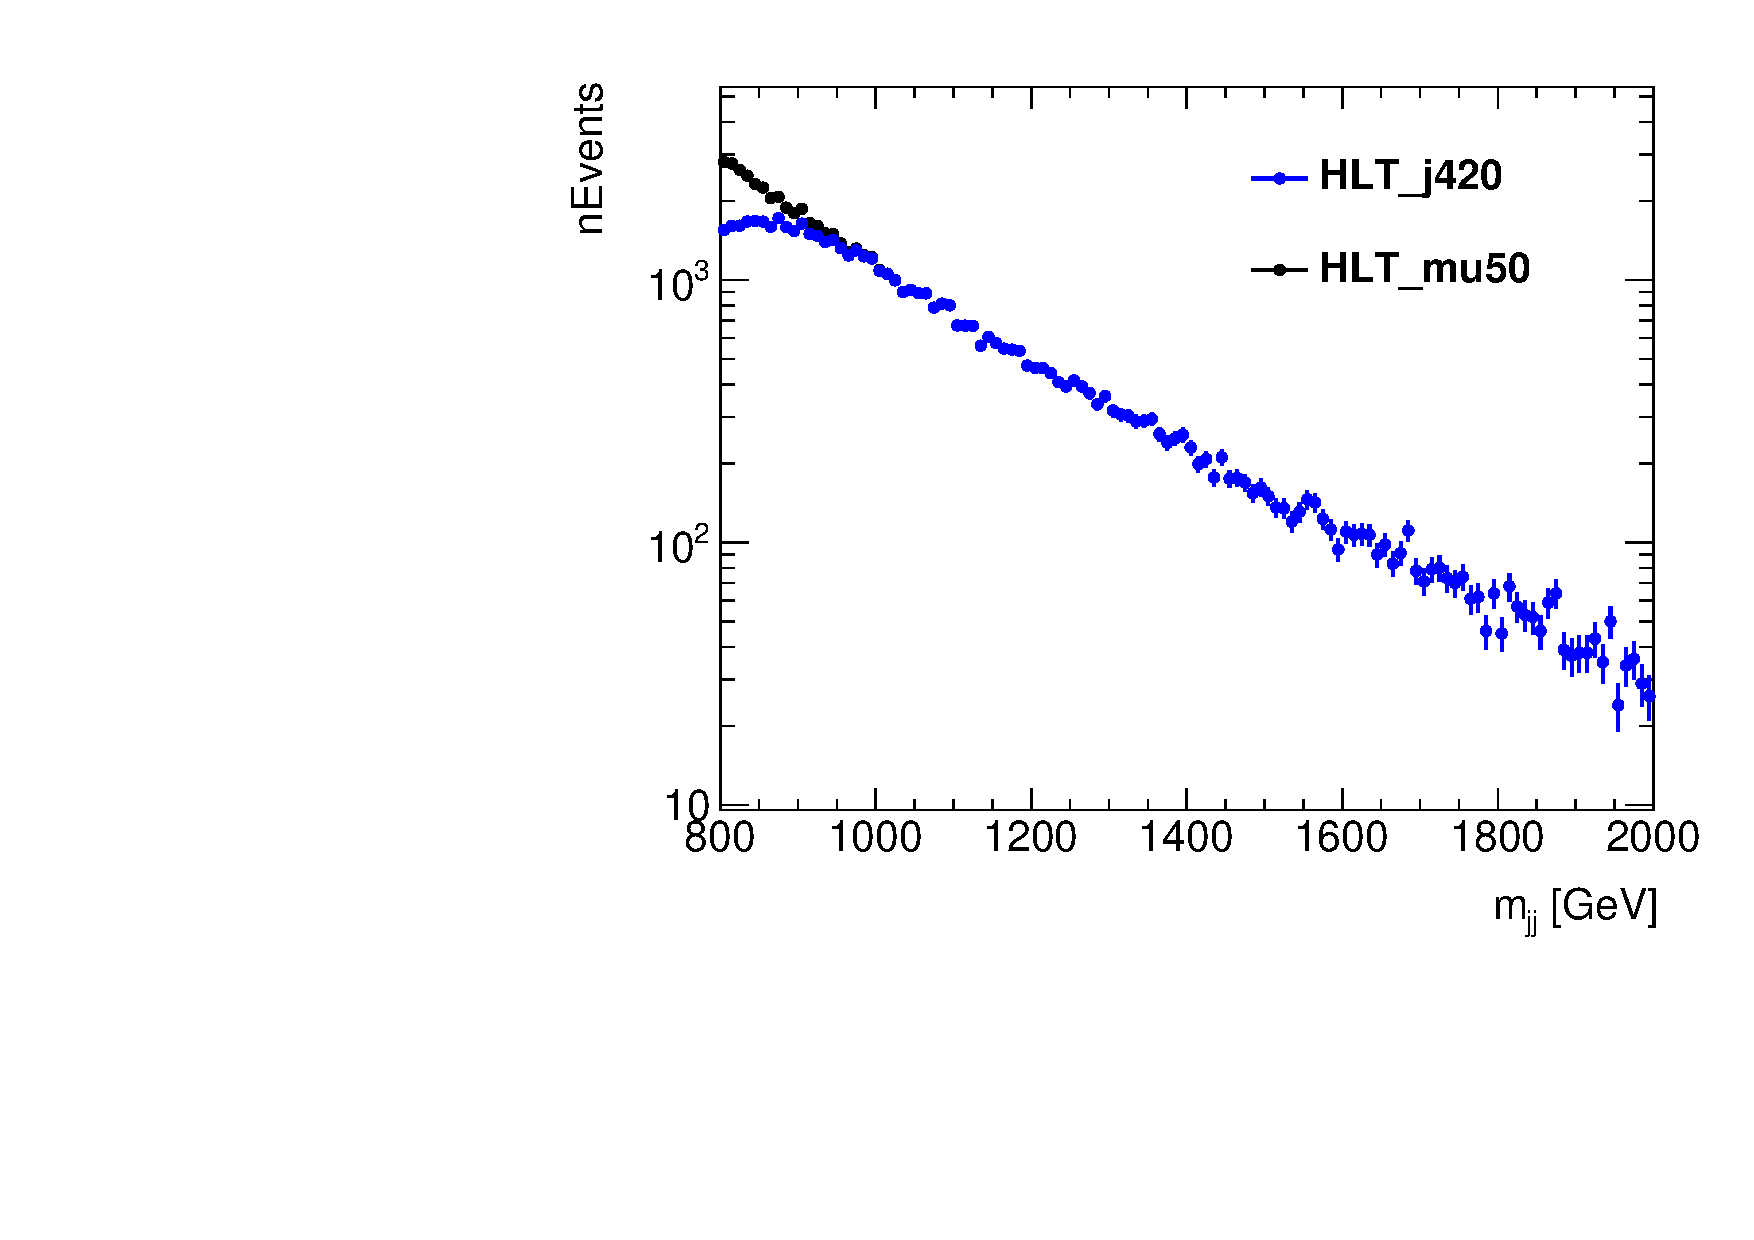
\includegraphics[width=0.48\columnwidth]{figures/massturnon/app_triggerturnon/mjj_gg_turnon_yStar0p6_Data18}}
        \\
        \subfigure[$\geq$1 g-tag]{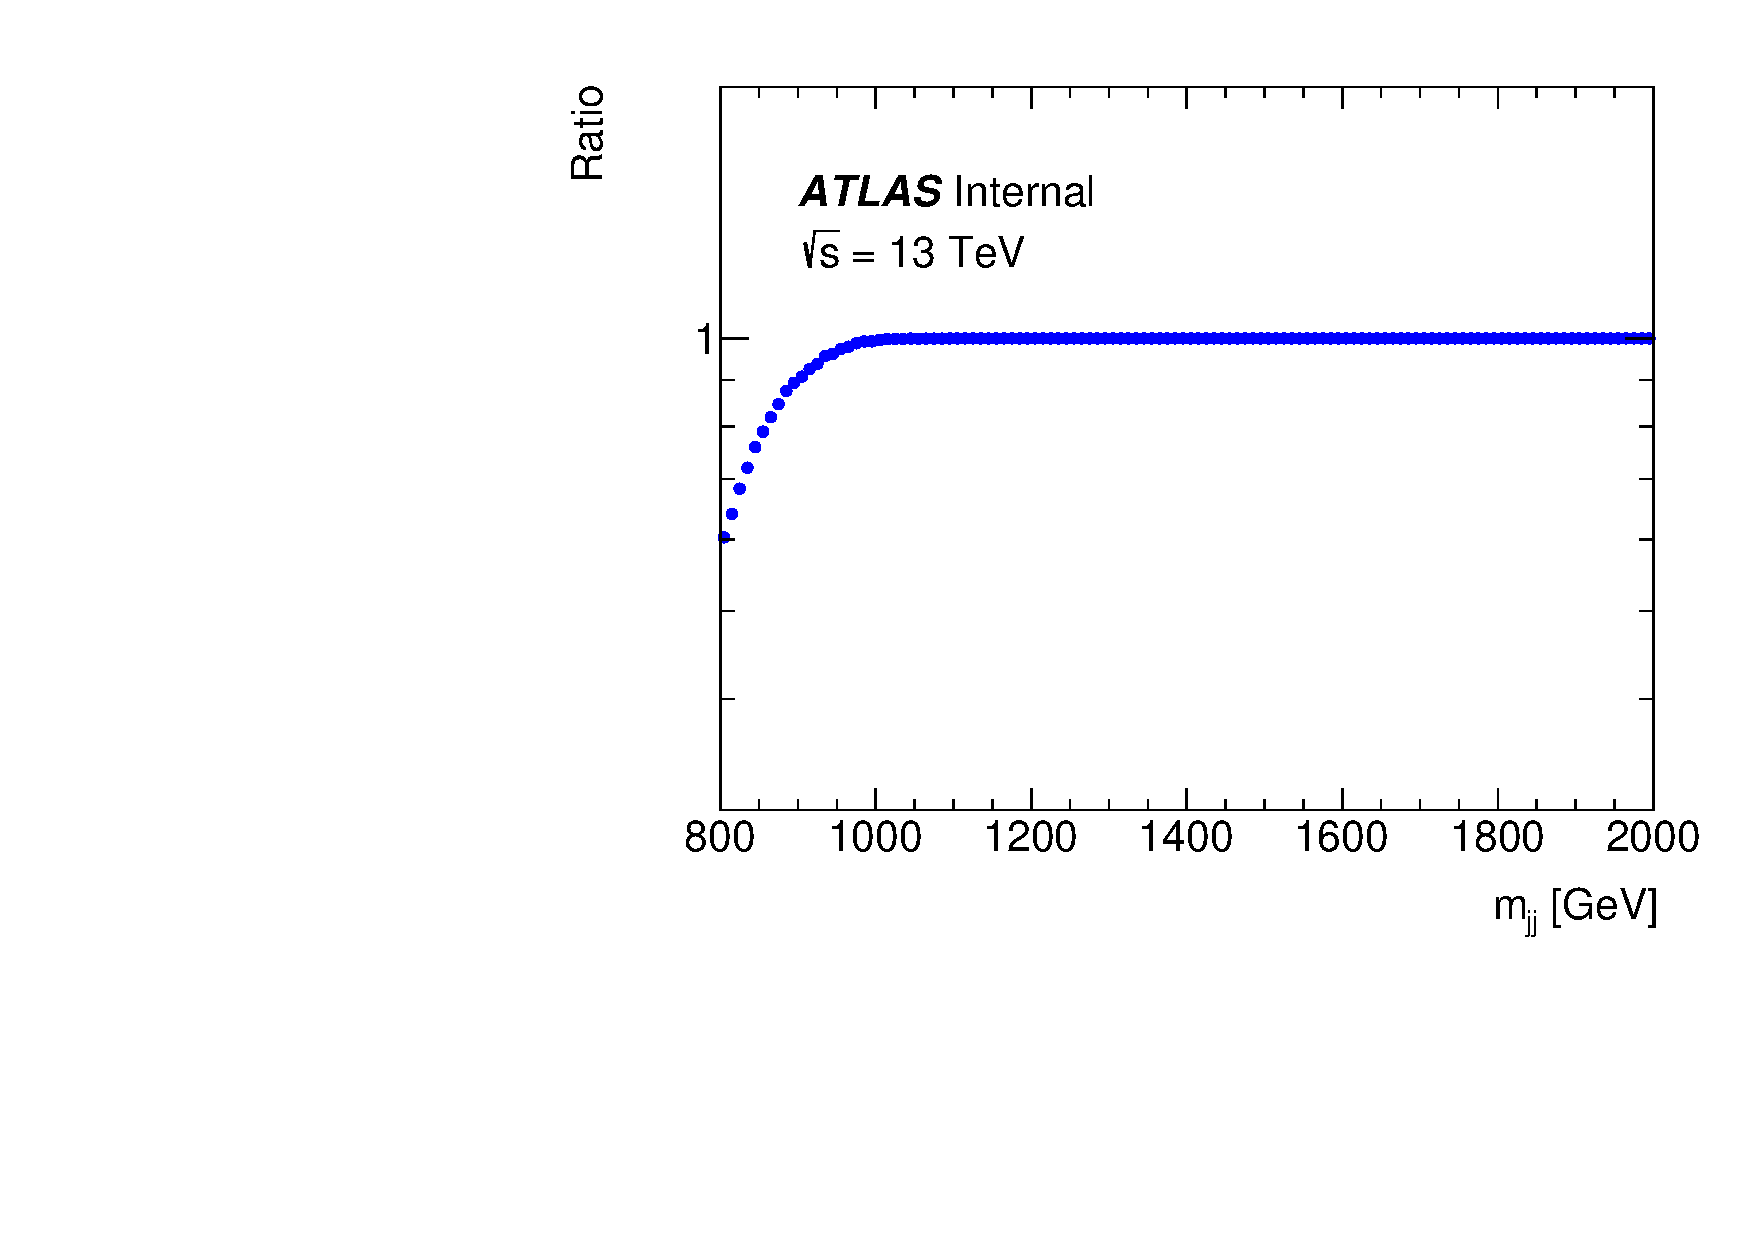
\includegraphics[width=0.48\columnwidth]{figures/massturnon/app_triggerturnon/Ratio_mjj_qg_turnon_yStar0p6_Data18}}
        \subfigure[2 g-tag]{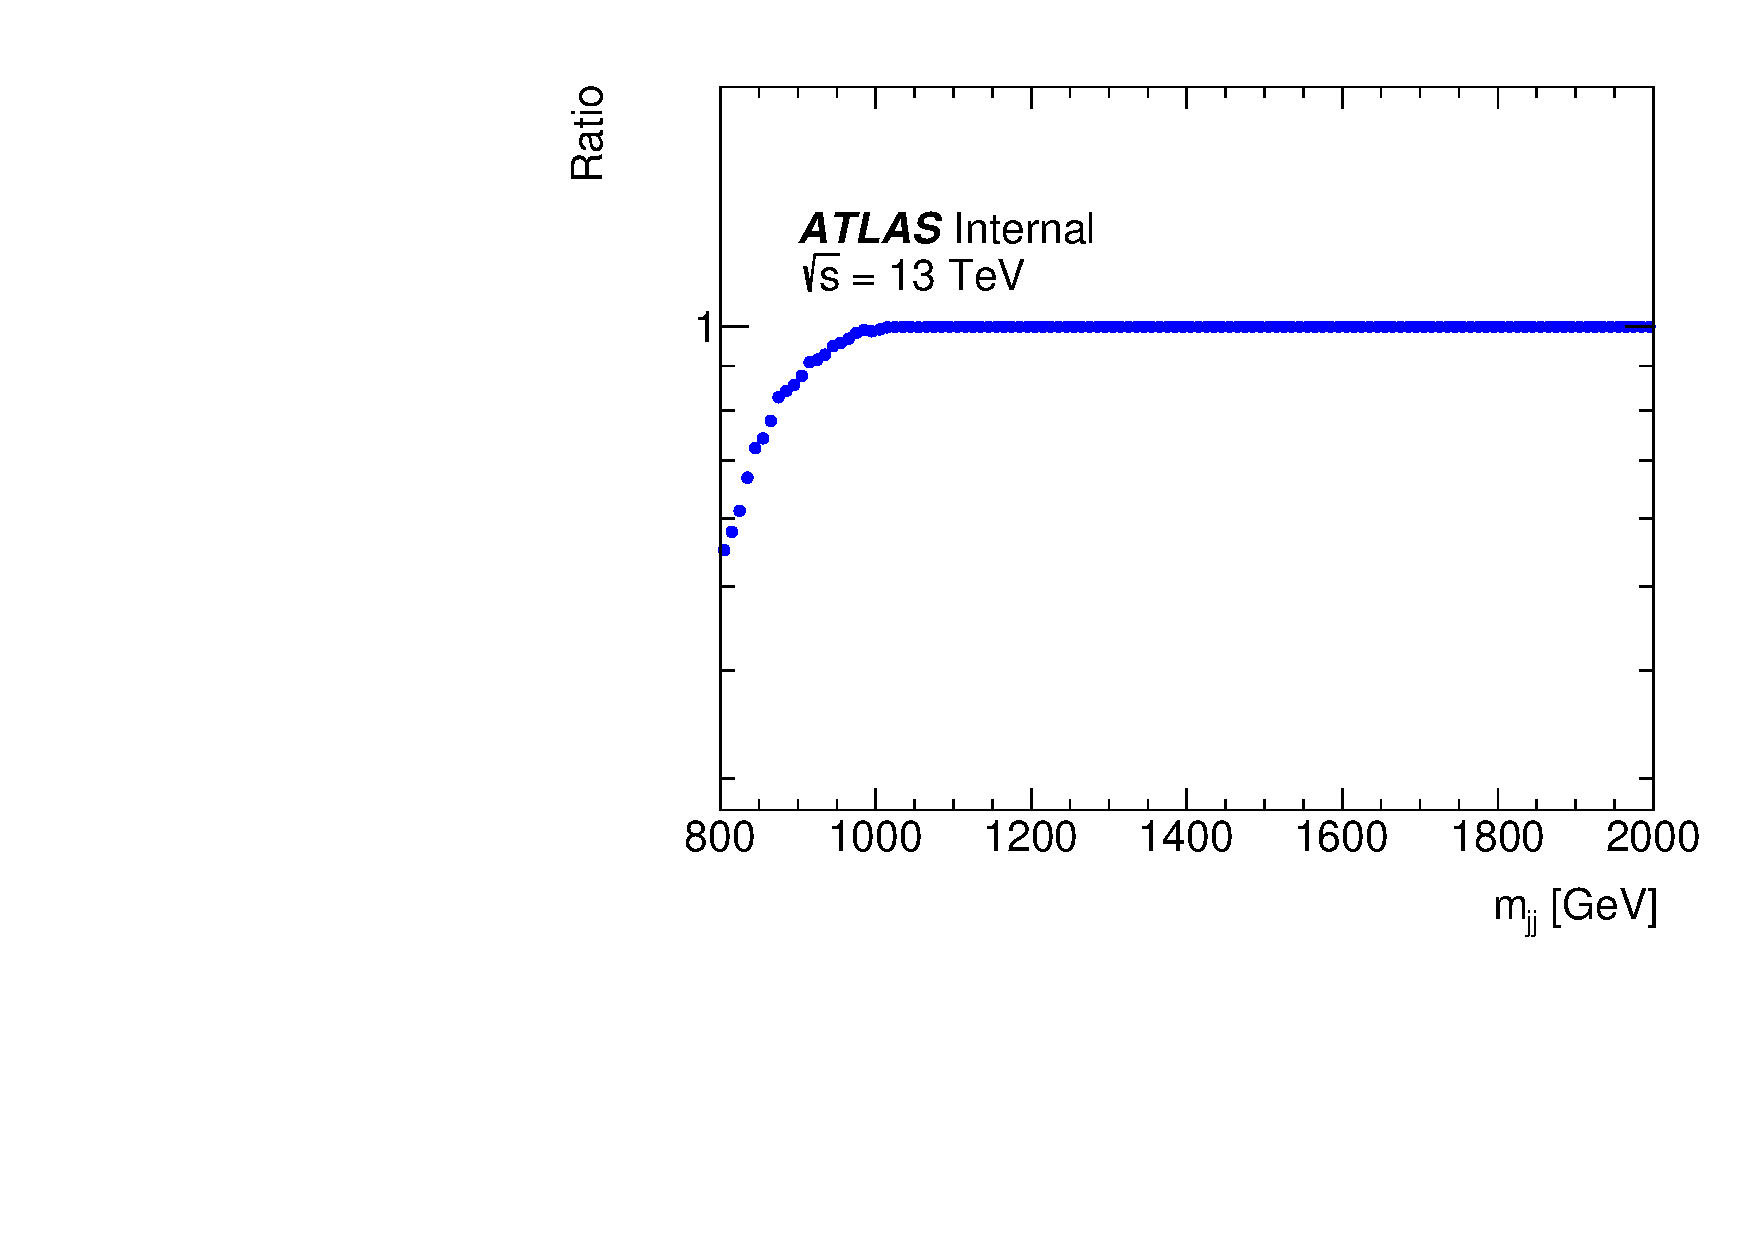
\includegraphics[width=0.48\columnwidth]{figures/massturnon/app_triggerturnon/Ratio_mjj_gg_turnon_yStar0p6_Data18}}

        \caption{Efficiencies as a function of \mjj\ for $|\ystar|<0.6$ using HLT\_j420 compared with HLT\_mu50 in the case of comparison of mass spectra with
        (a) $\geq$1 g-tag, (b) 2 g-tag and the ratio between the two (c) $\geq$1 g-tag and (d) 2 g-tag for 2018 data.}
        \label{fig:trigger-yStar0p6-Data18}
\end{figure}

\begin{figure}[htbp]
        \centering
        \subfigure[$\geq$1 g-tag]{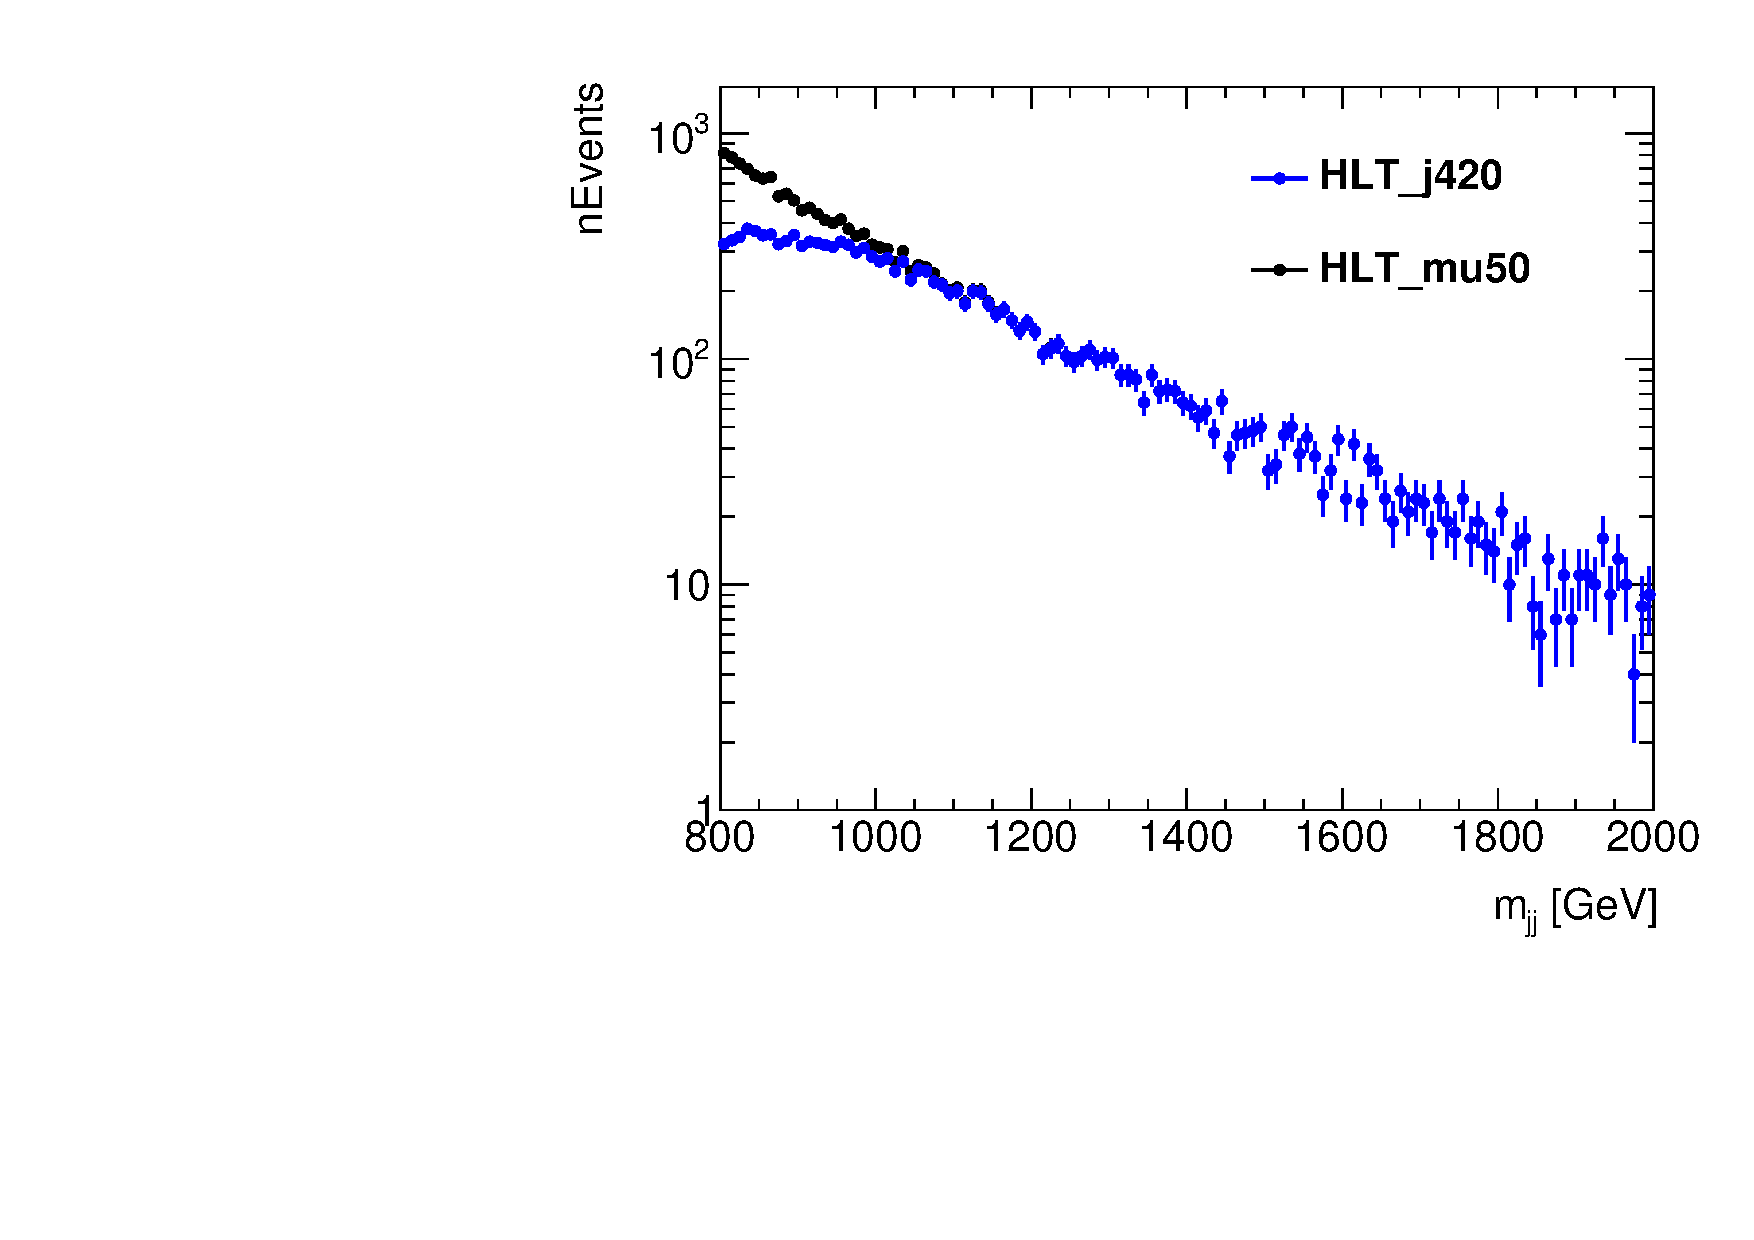
\includegraphics[width=0.48\columnwidth]{figures/massturnon/app_triggerturnon/mjj_qg_turnon_yStar0p8_Data15}}
        \subfigure[2 g-tag]{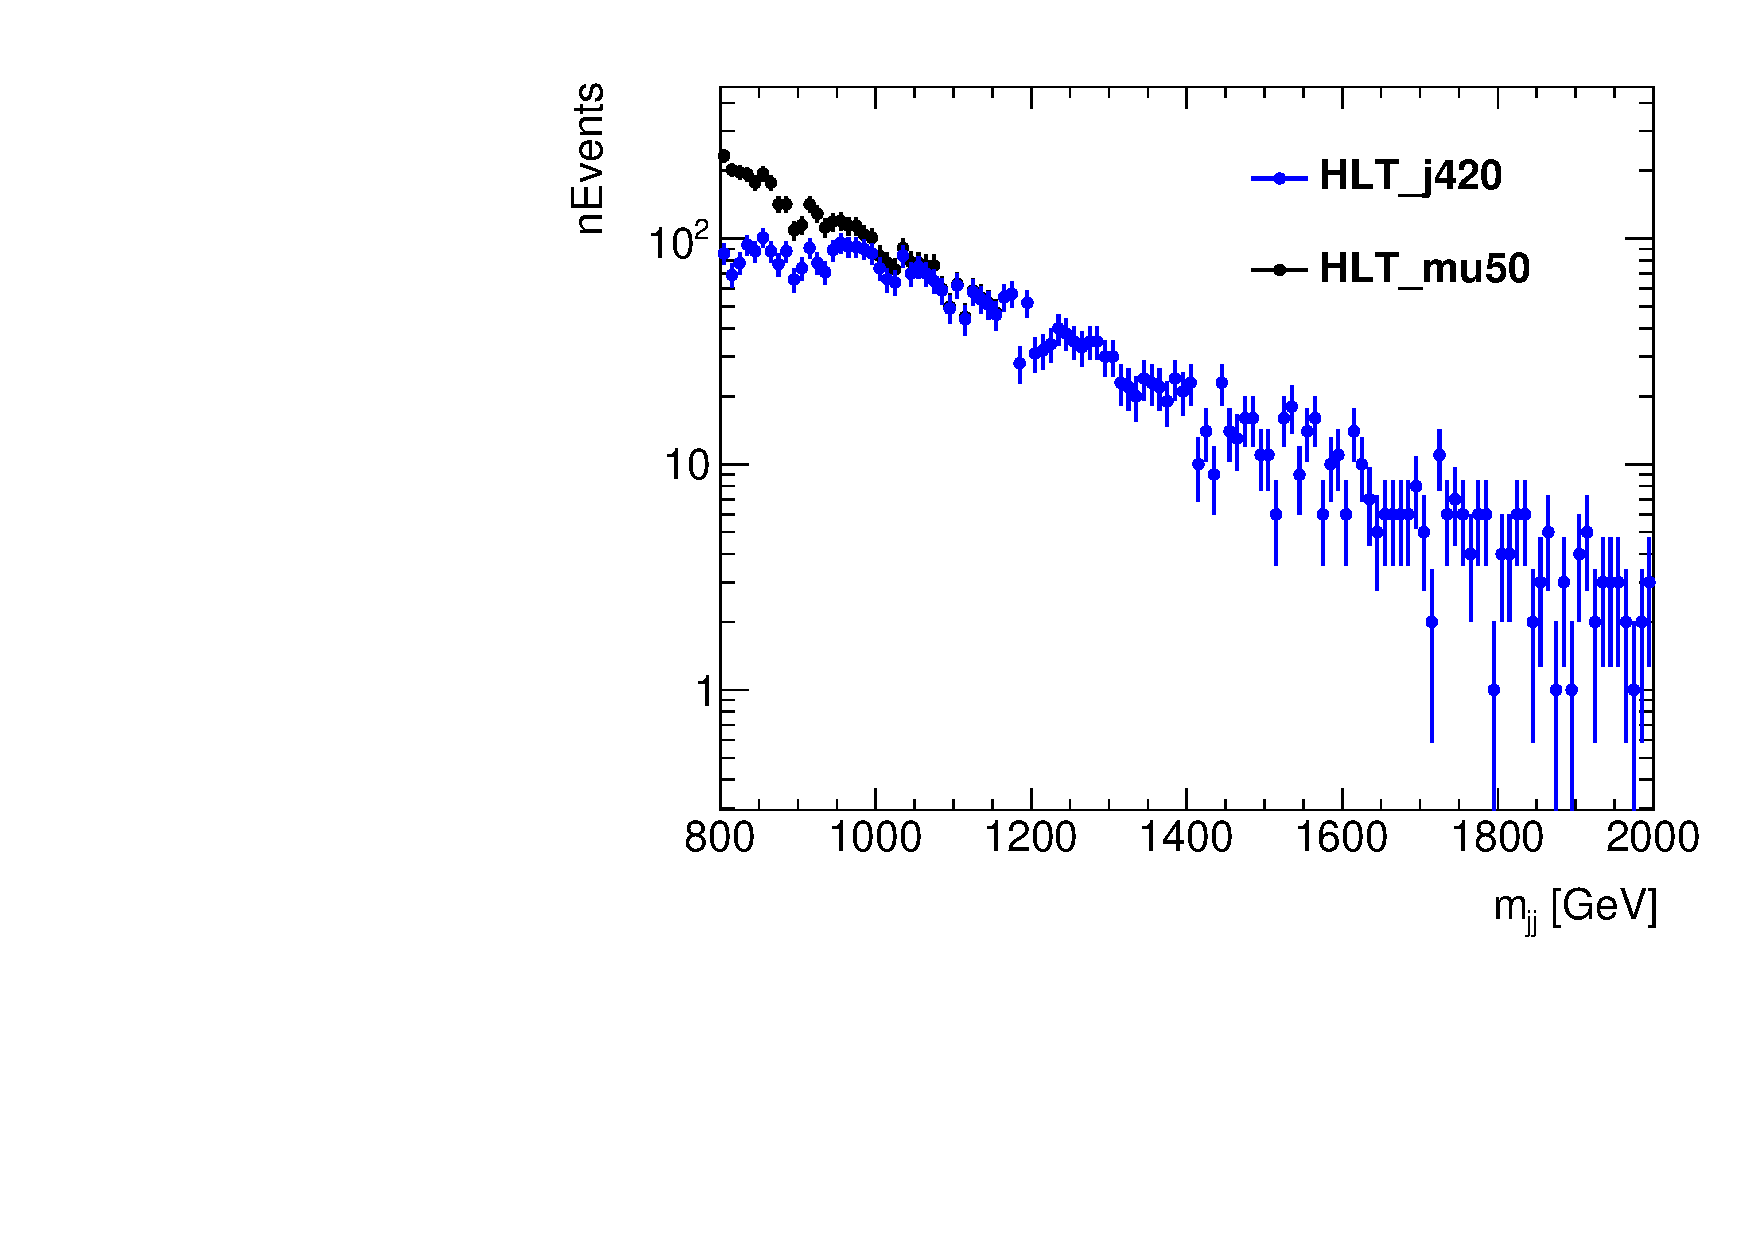
\includegraphics[width=0.48\columnwidth]{figures/massturnon/app_triggerturnon/mjj_gg_turnon_yStar0p8_Data15}}
        \\
        \subfigure[$\geq$1 g-tag]{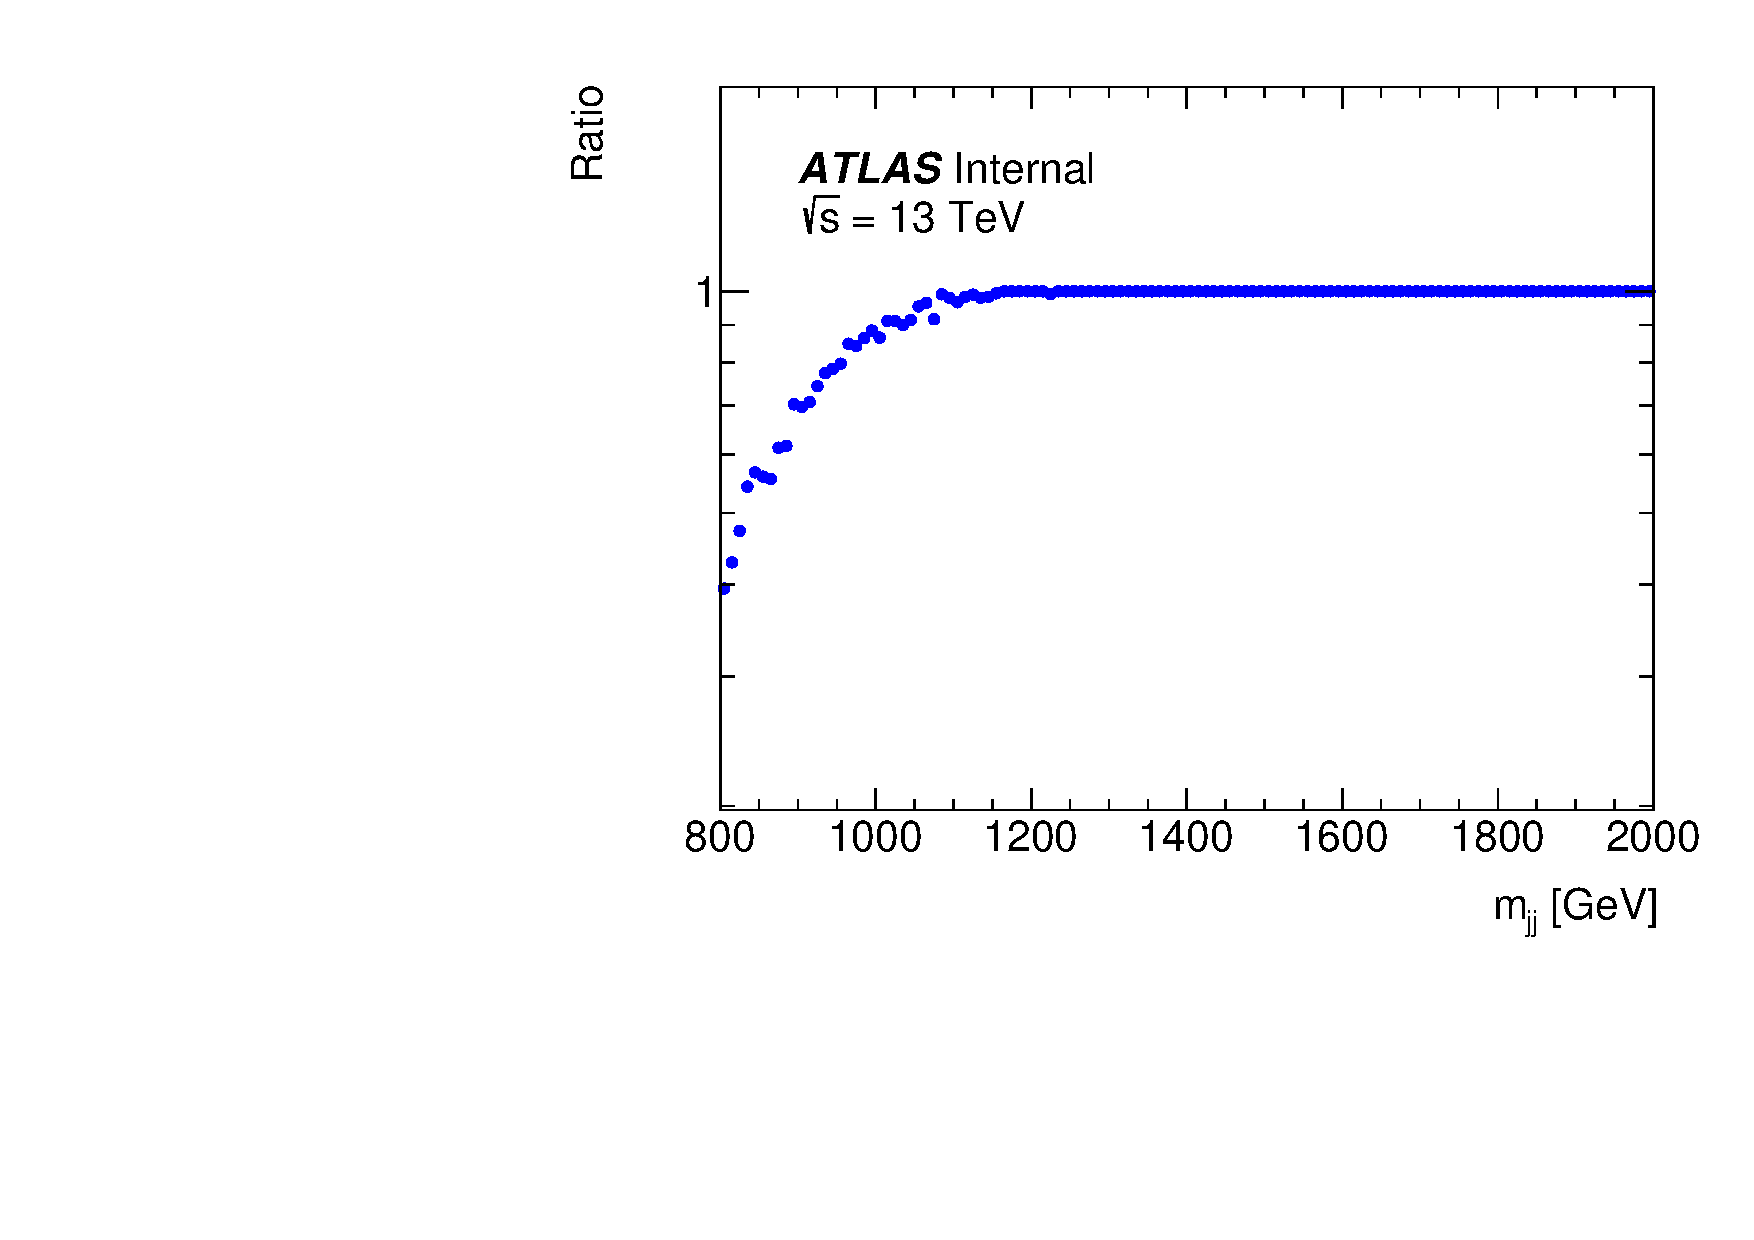
\includegraphics[width=0.48\columnwidth]{figures/massturnon/app_triggerturnon/Ratio_mjj_qg_turnon_yStar0p8_Data15}}
        \subfigure[2 g-tag]{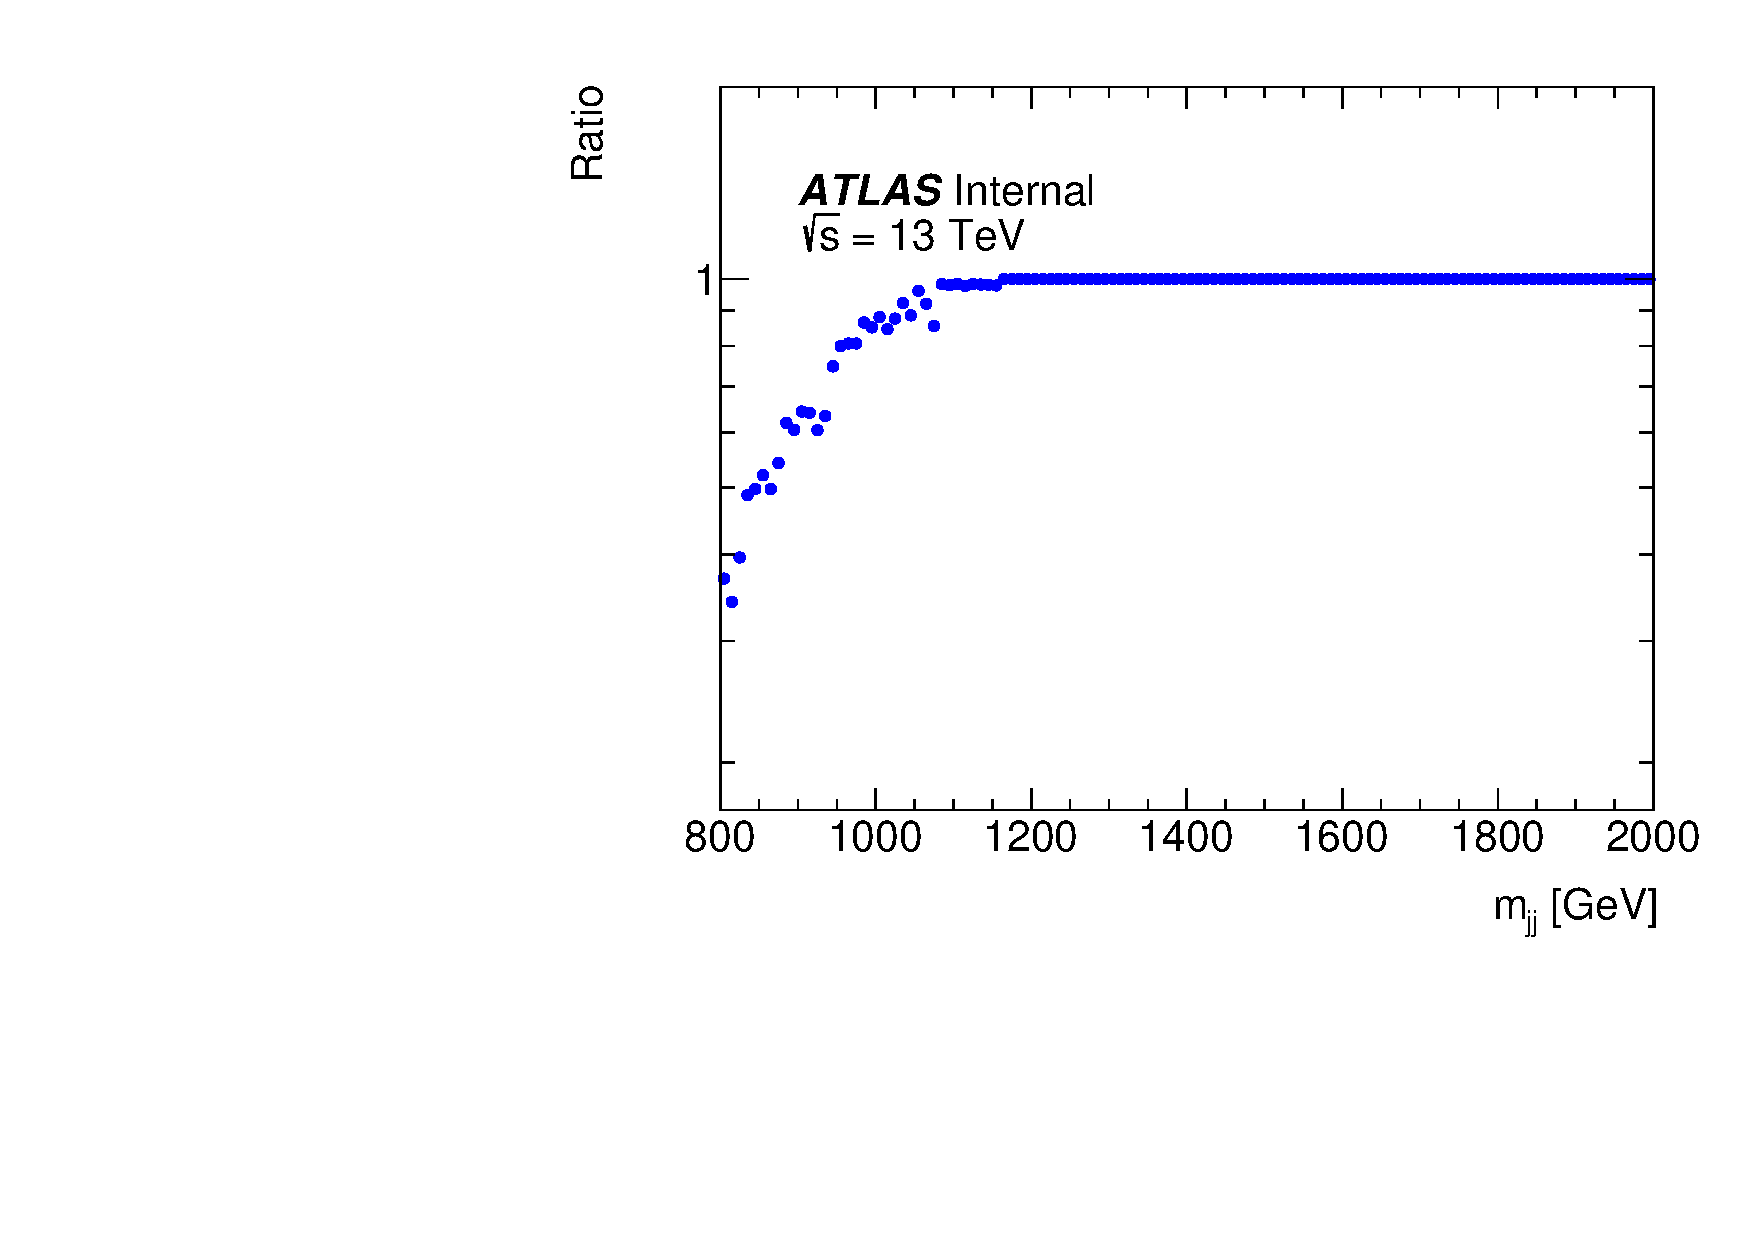
\includegraphics[width=0.48\columnwidth]{figures/massturnon/app_triggerturnon/Ratio_mjj_gg_turnon_yStar0p8_Data15}}

        \caption{Efficiencies as a function of \mjj\ for $|\ystar|<0.8$ using HLT\_j420 compared with HLT\_mu50 in the case of comparison of mass spectra with
        (a) $\geq$1 g-tag, (b) 2 g-tag and the ratio between the two (c) $\geq$1 g-tag and (d) 2 g-tag for 2015 data.}
        \label{fig:trigger-yStar0p8-Data15}
\end{figure}

\begin{figure}[htbp]
        \centering
        \subfigure[$\geq$1 g-tag]{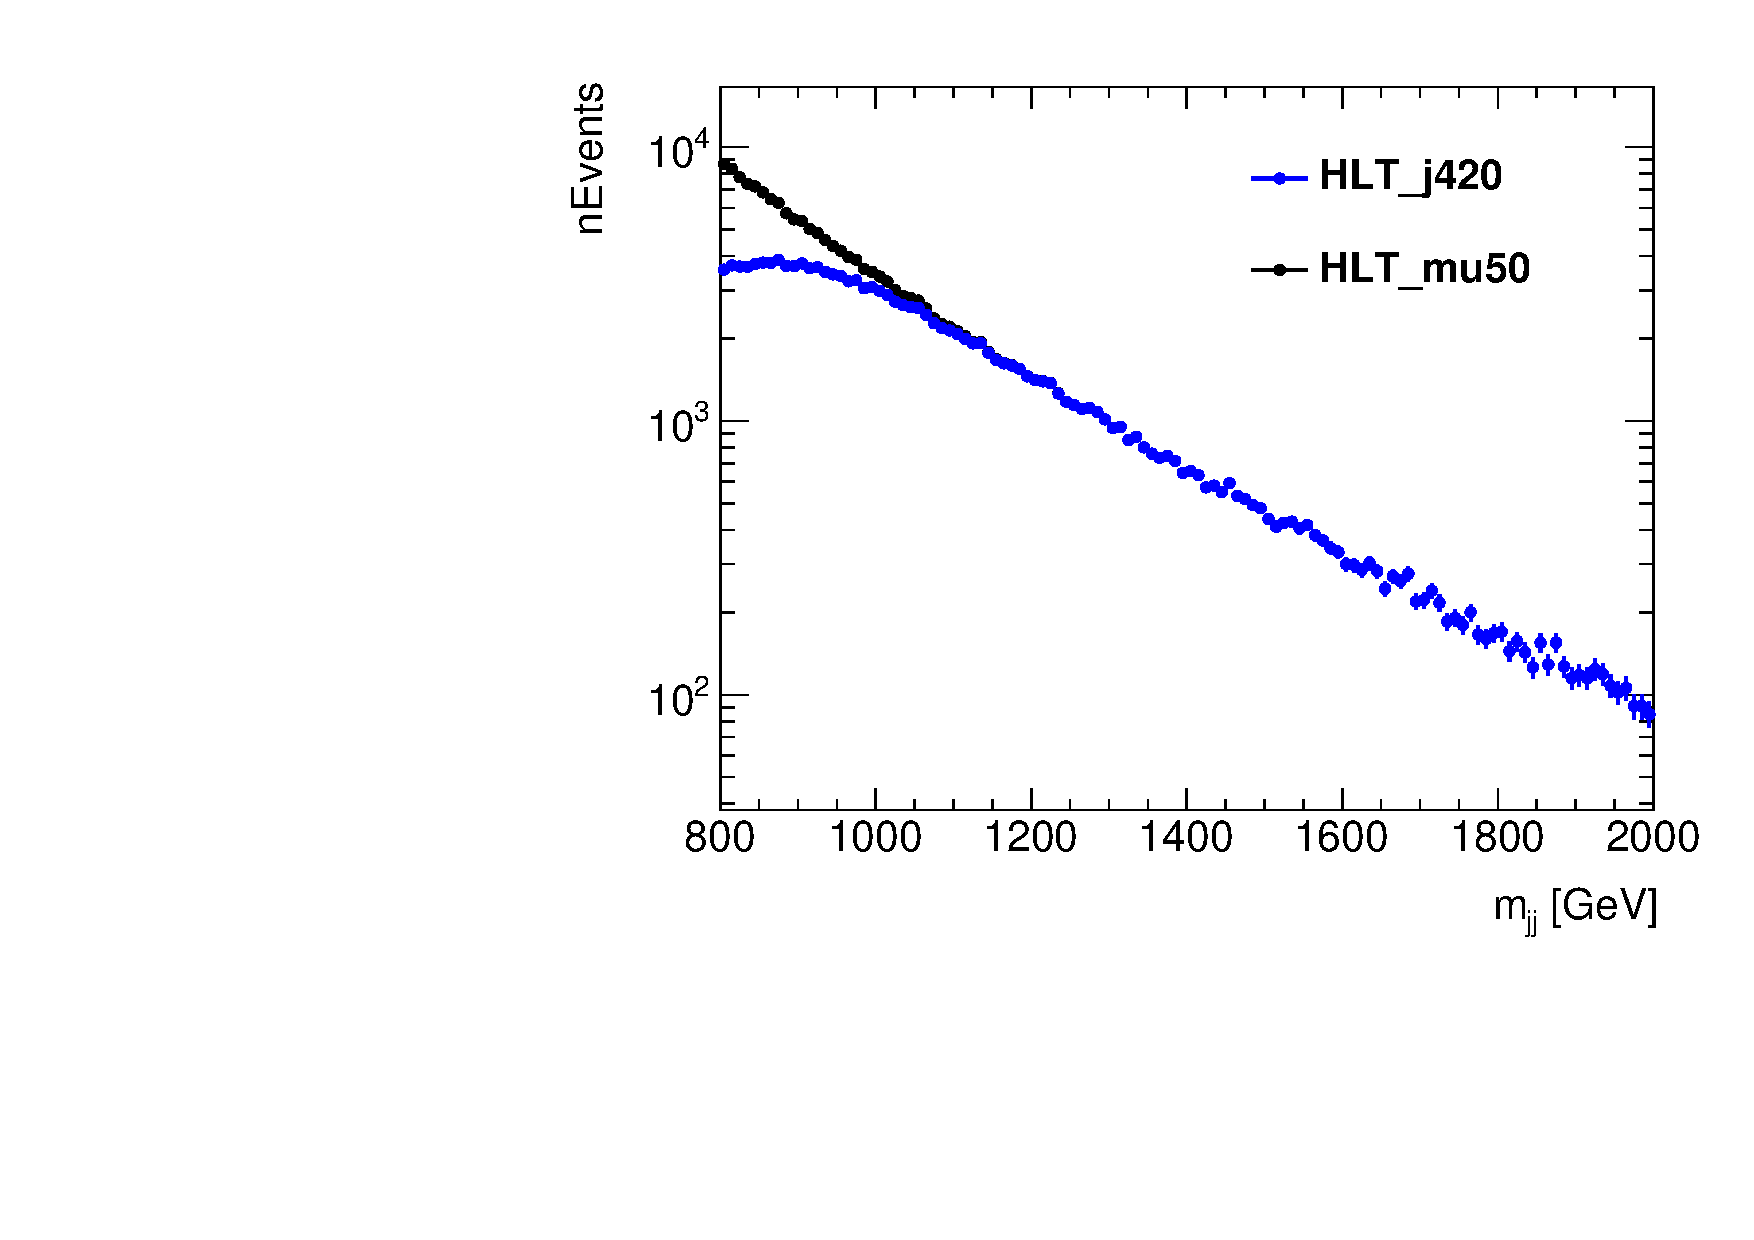
\includegraphics[width=0.48\columnwidth]{figures/massturnon/app_triggerturnon/mjj_qg_turnon_yStar0p8_Data16}}
        \subfigure[2 g-tag]{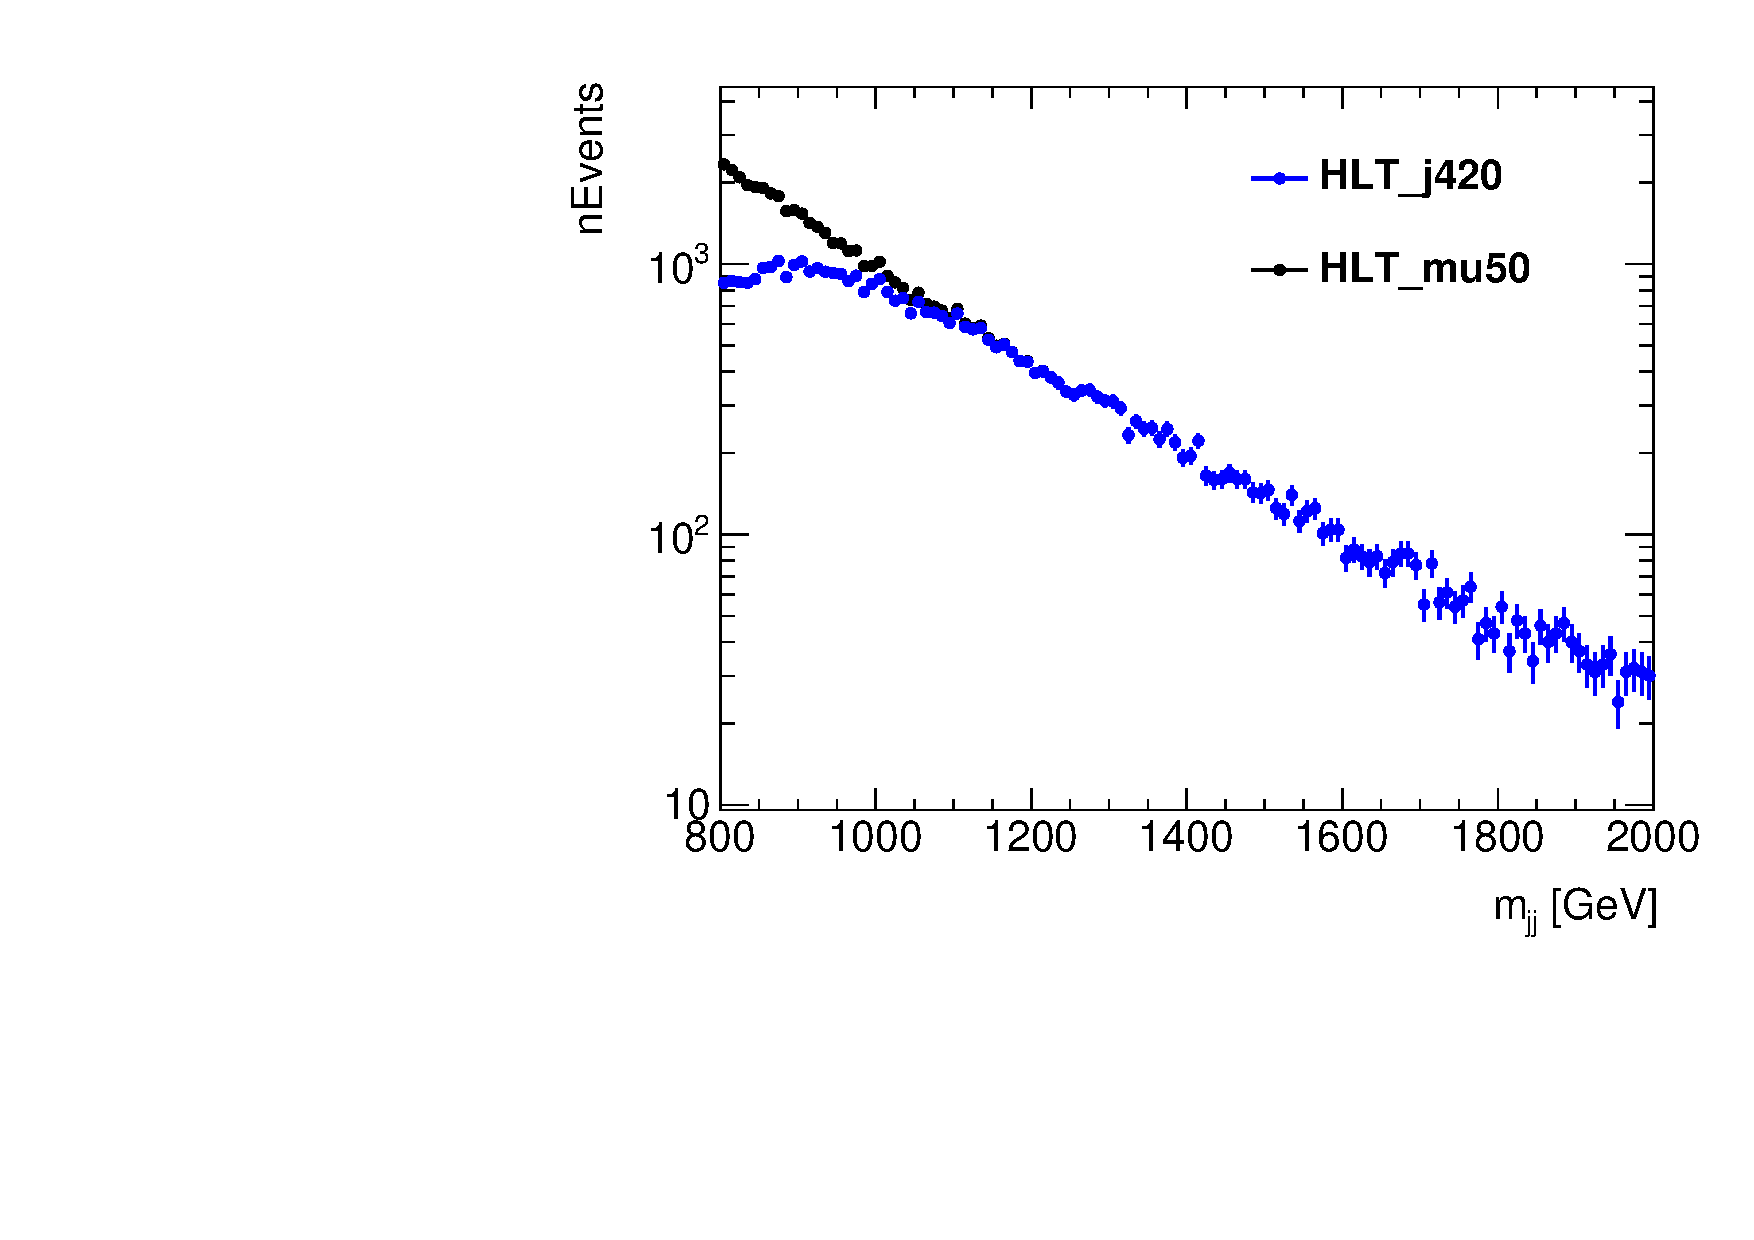
\includegraphics[width=0.48\columnwidth]{figures/massturnon/app_triggerturnon/mjj_gg_turnon_yStar0p8_Data16}}
        \\
        \subfigure[$\geq$1 g-tag]{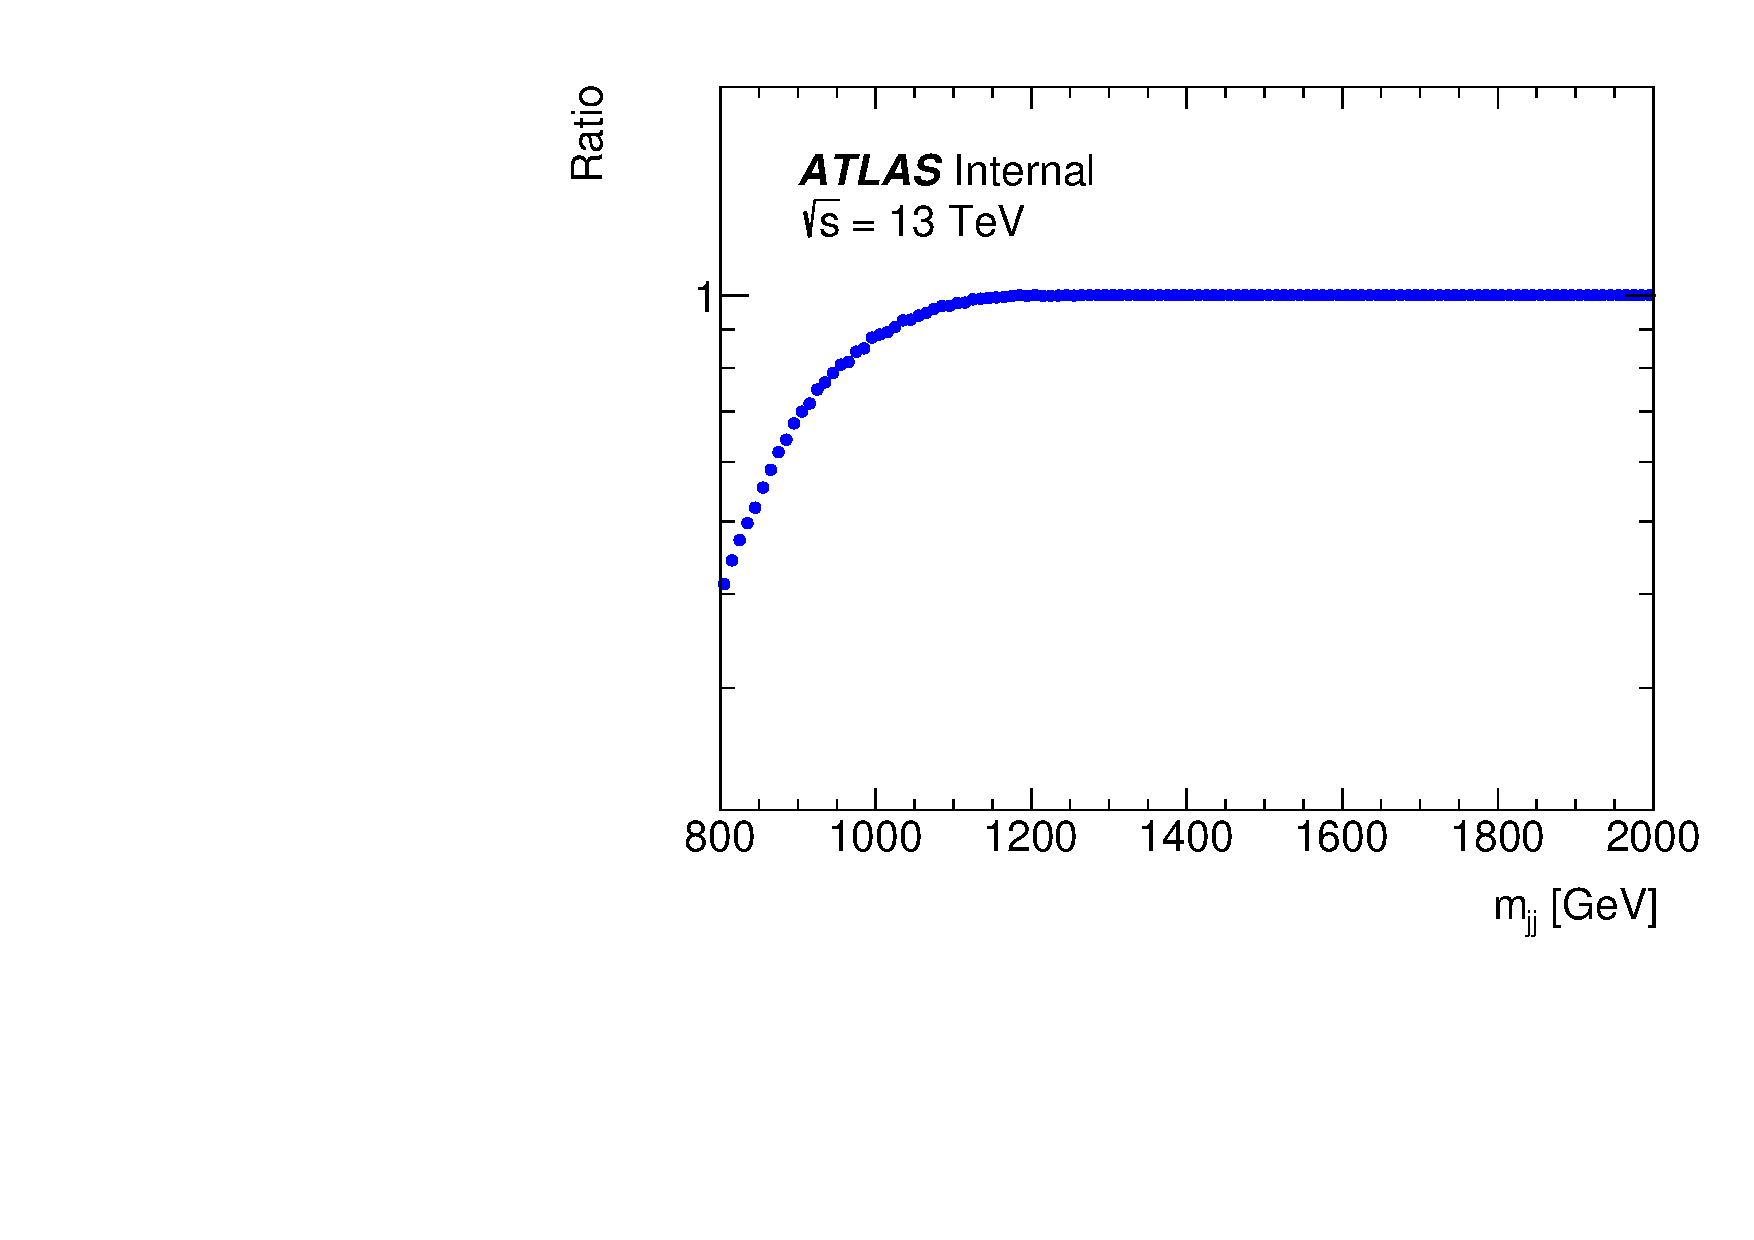
\includegraphics[width=0.48\columnwidth]{figures/massturnon/app_triggerturnon/Ratio_mjj_qg_turnon_yStar0p8_Data16}}
        \subfigure[2 g-tag]{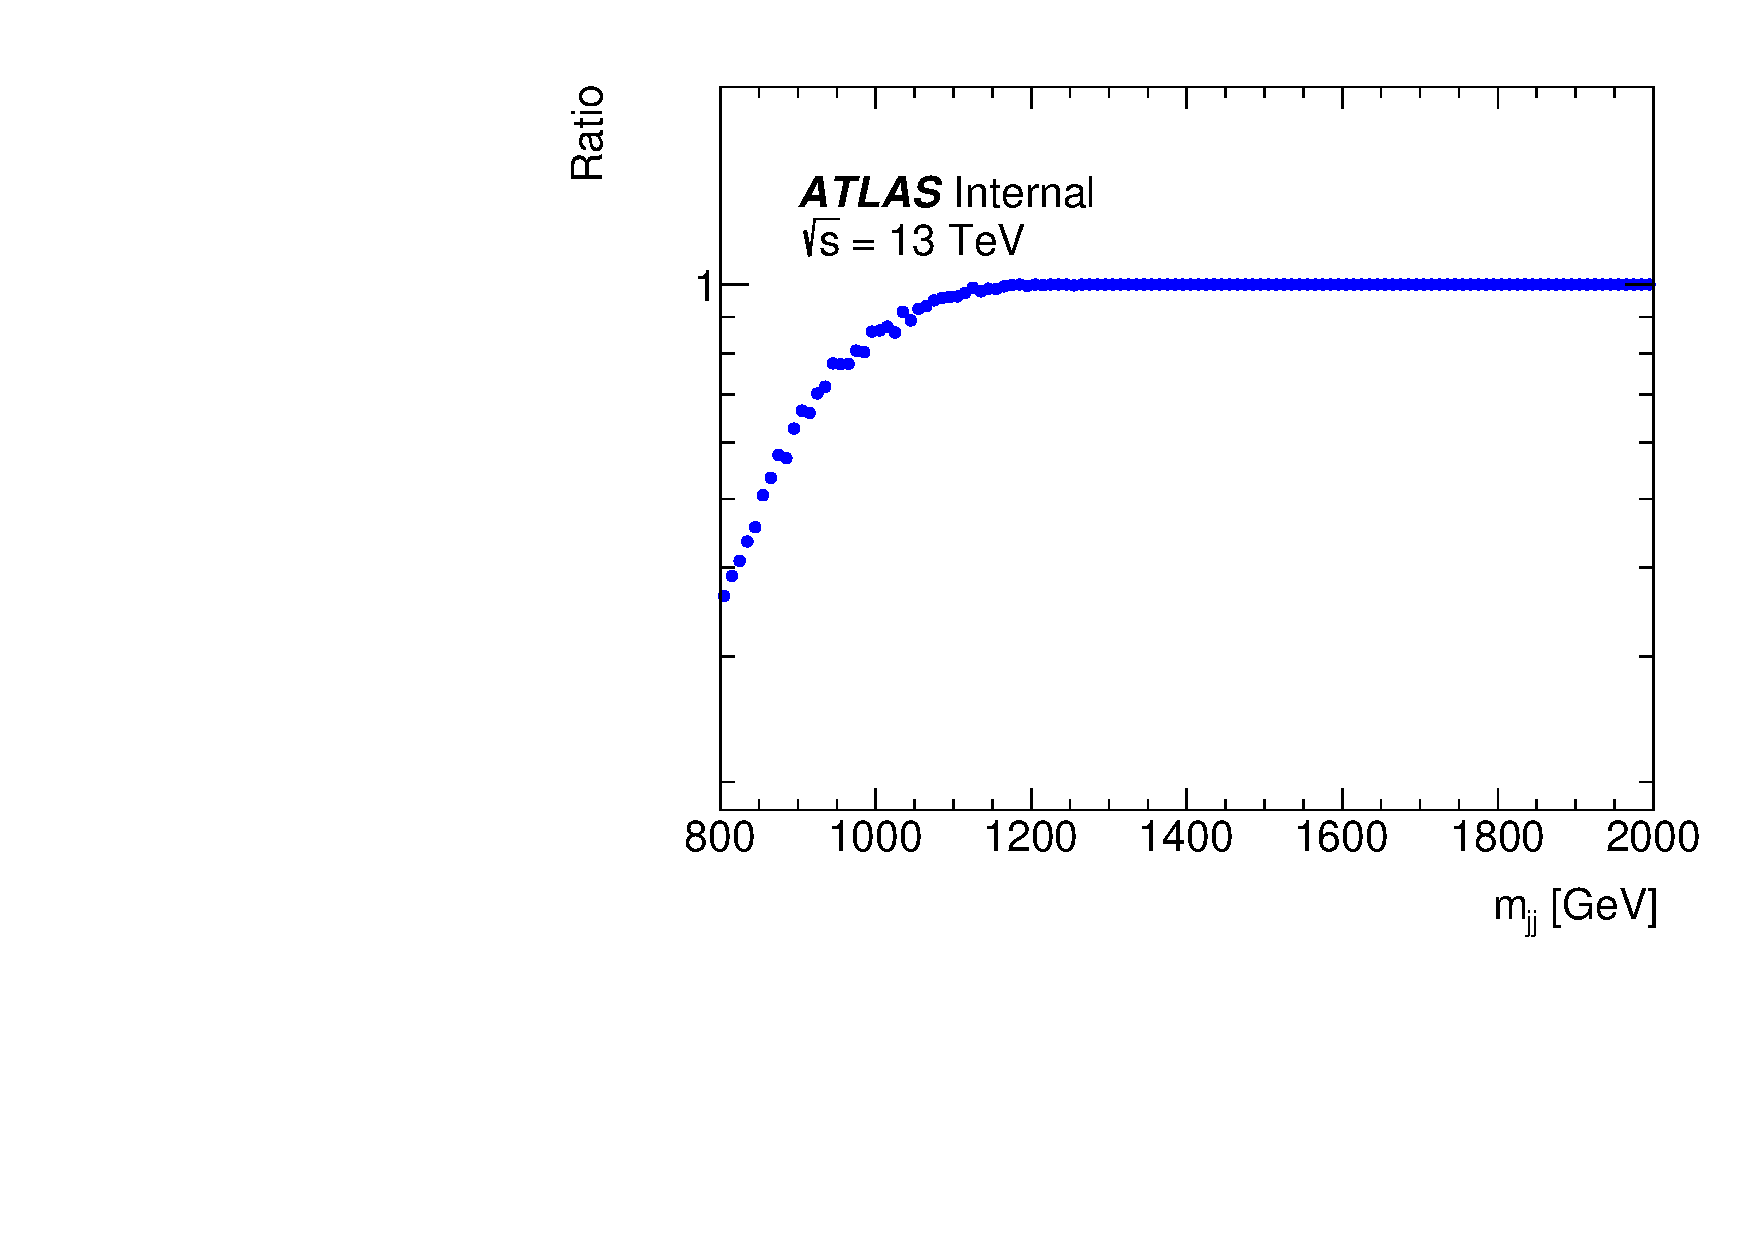
\includegraphics[width=0.48\columnwidth]{figures/massturnon/app_triggerturnon/Ratio_mjj_gg_turnon_yStar0p8_Data16}}

        \caption{Efficiencies as a function of \mjj\ for $|\ystar|<0.8$ using HLT\_j420 compared with HLT\_mu50 in the case of comparison of mass spectra with
        (a) $\geq$1 g-tag, (b) 2 g-tag and the ratio between the two (c) $\geq$1 g-tag and (d) 2 g-tag for 2016 data.}
\end{figure}

\begin{figure}[htbp]
        \centering
        \subfigure[$\geq$1 g-tag]{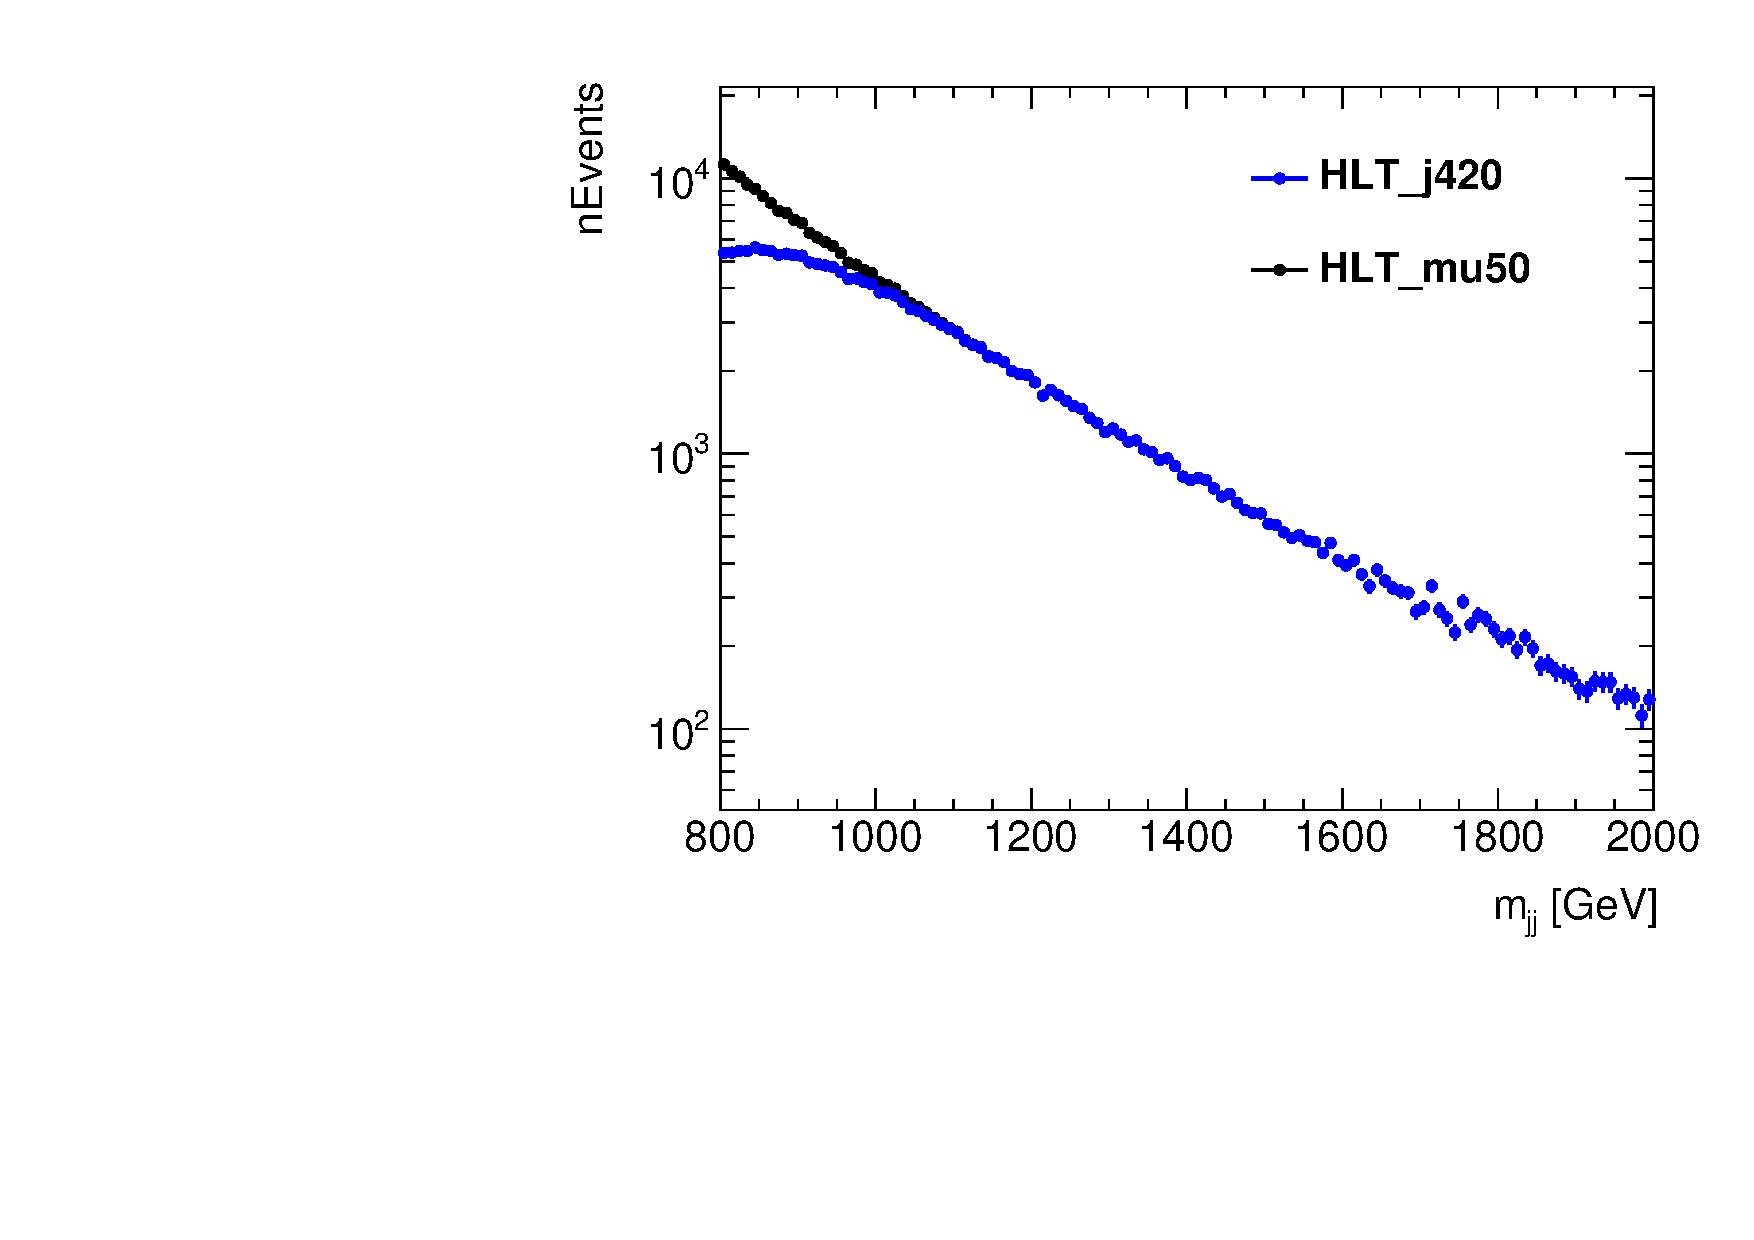
\includegraphics[width=0.48\columnwidth]{figures/massturnon/app_triggerturnon/mjj_qg_turnon_yStar0p8_Data17}}
        \subfigure[2 g-tag]{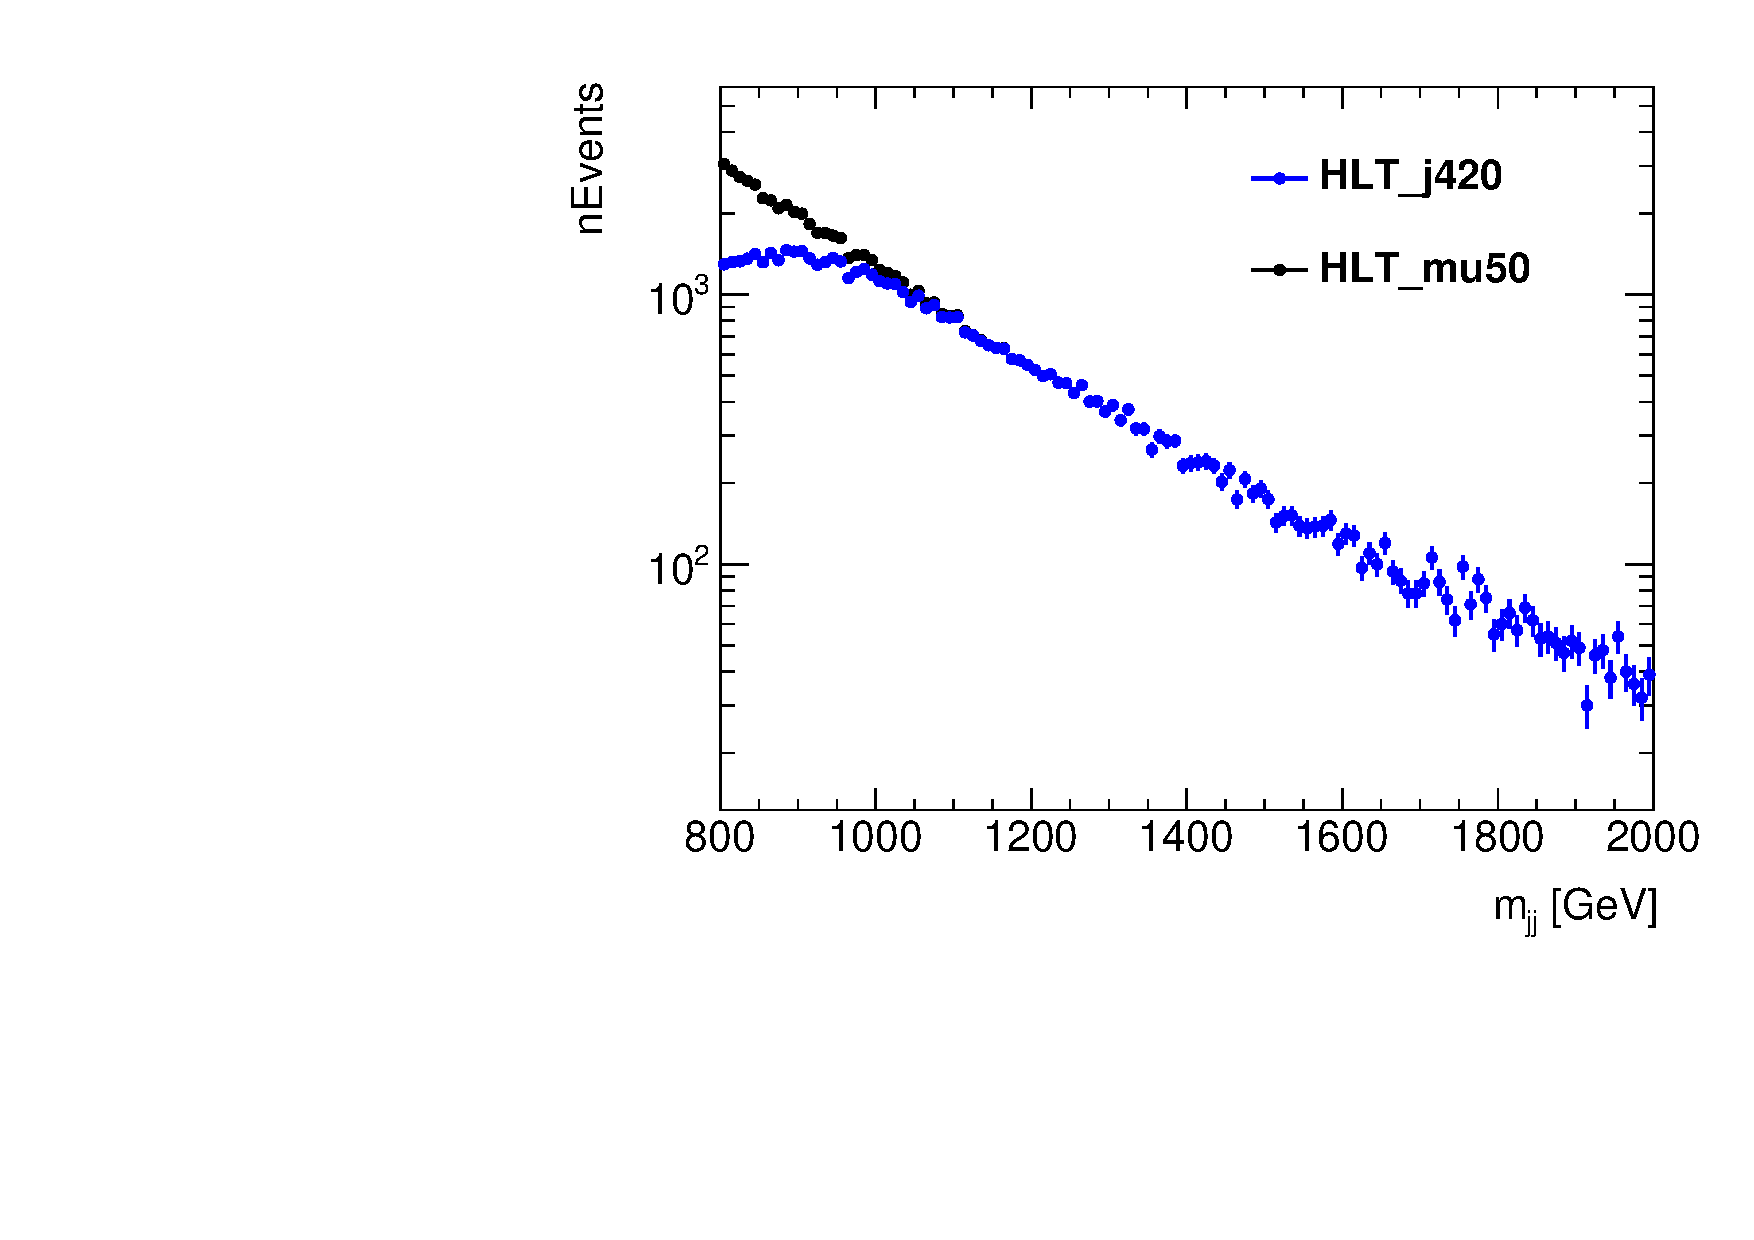
\includegraphics[width=0.48\columnwidth]{figures/massturnon/app_triggerturnon/mjj_gg_turnon_yStar0p8_Data17}}
        \\
        \subfigure[$\geq$1 g-tag]{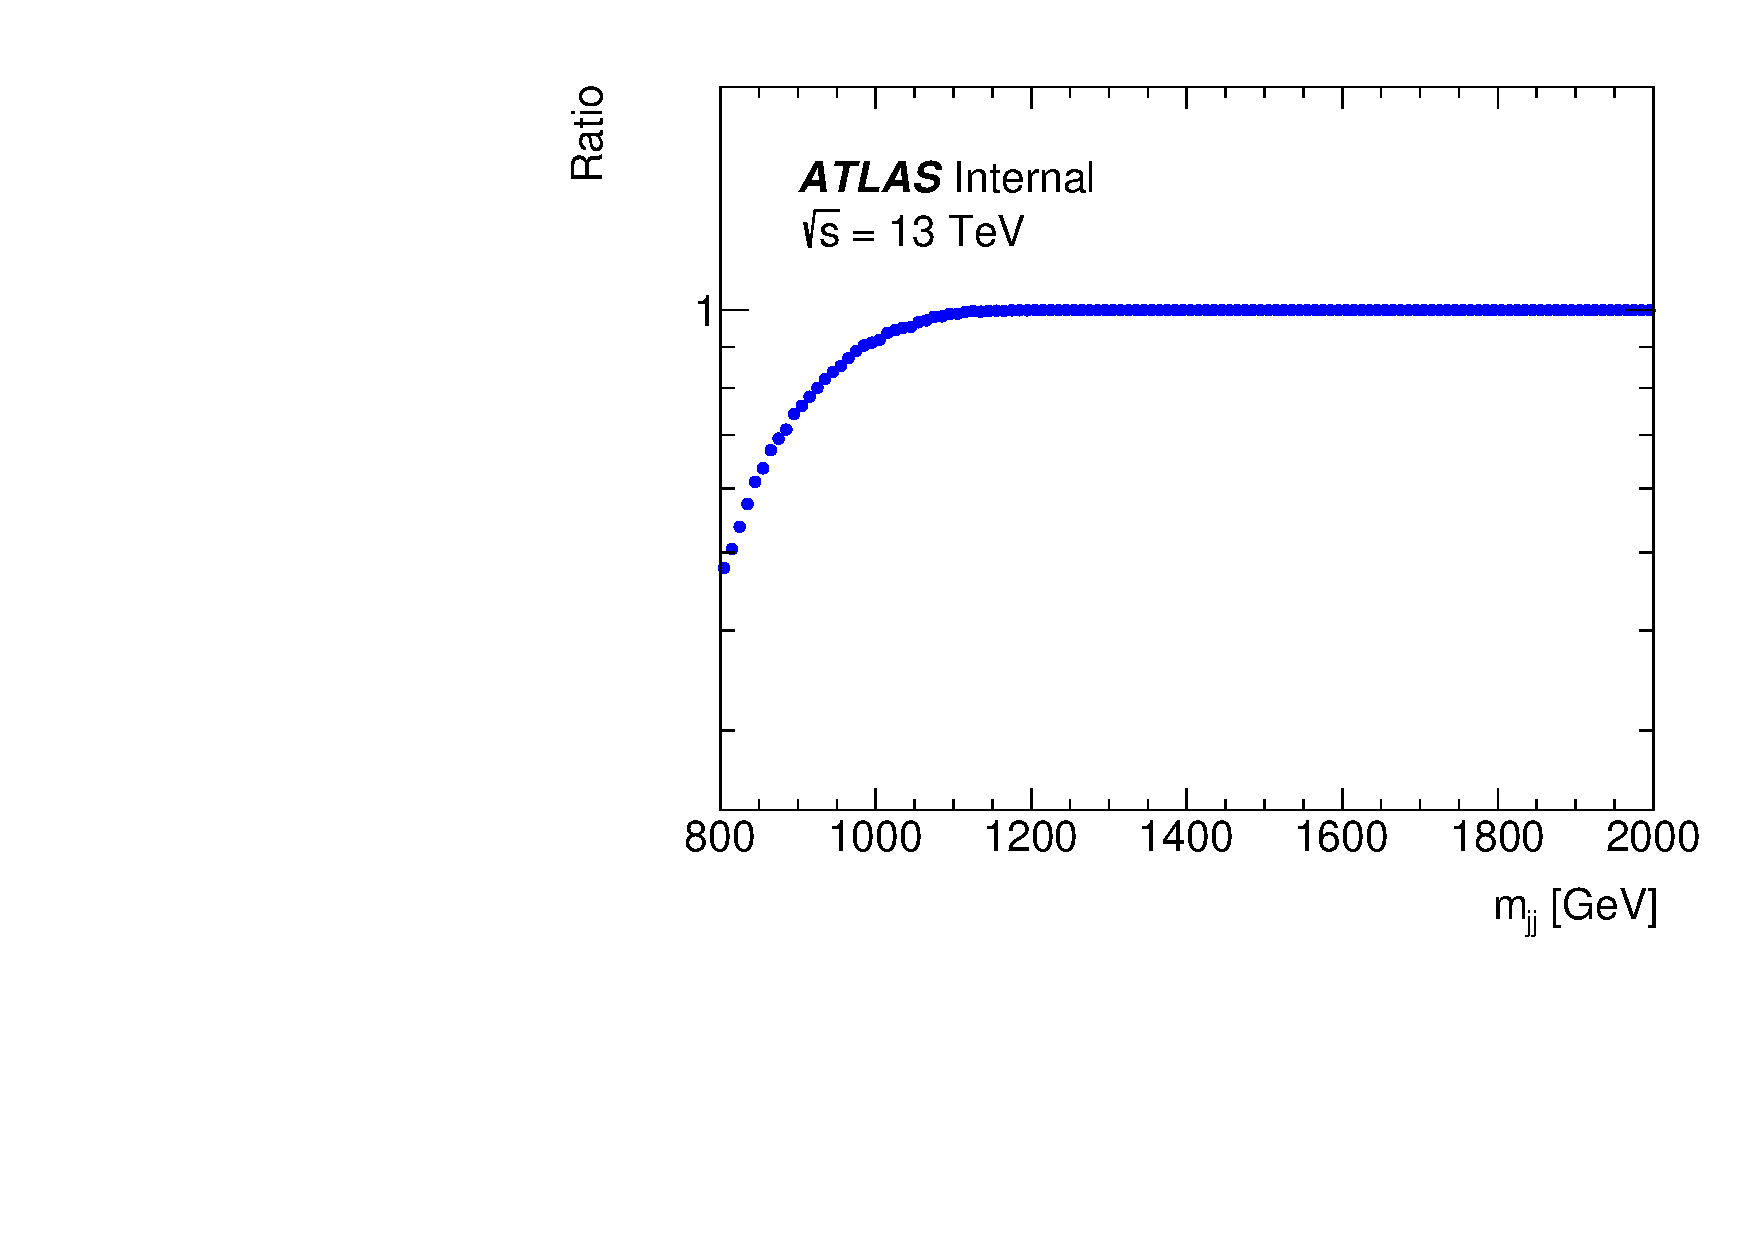
\includegraphics[width=0.48\columnwidth]{figures/massturnon/app_triggerturnon/Ratio_mjj_qg_turnon_yStar0p8_Data17}}
        \subfigure[2 g-tag]{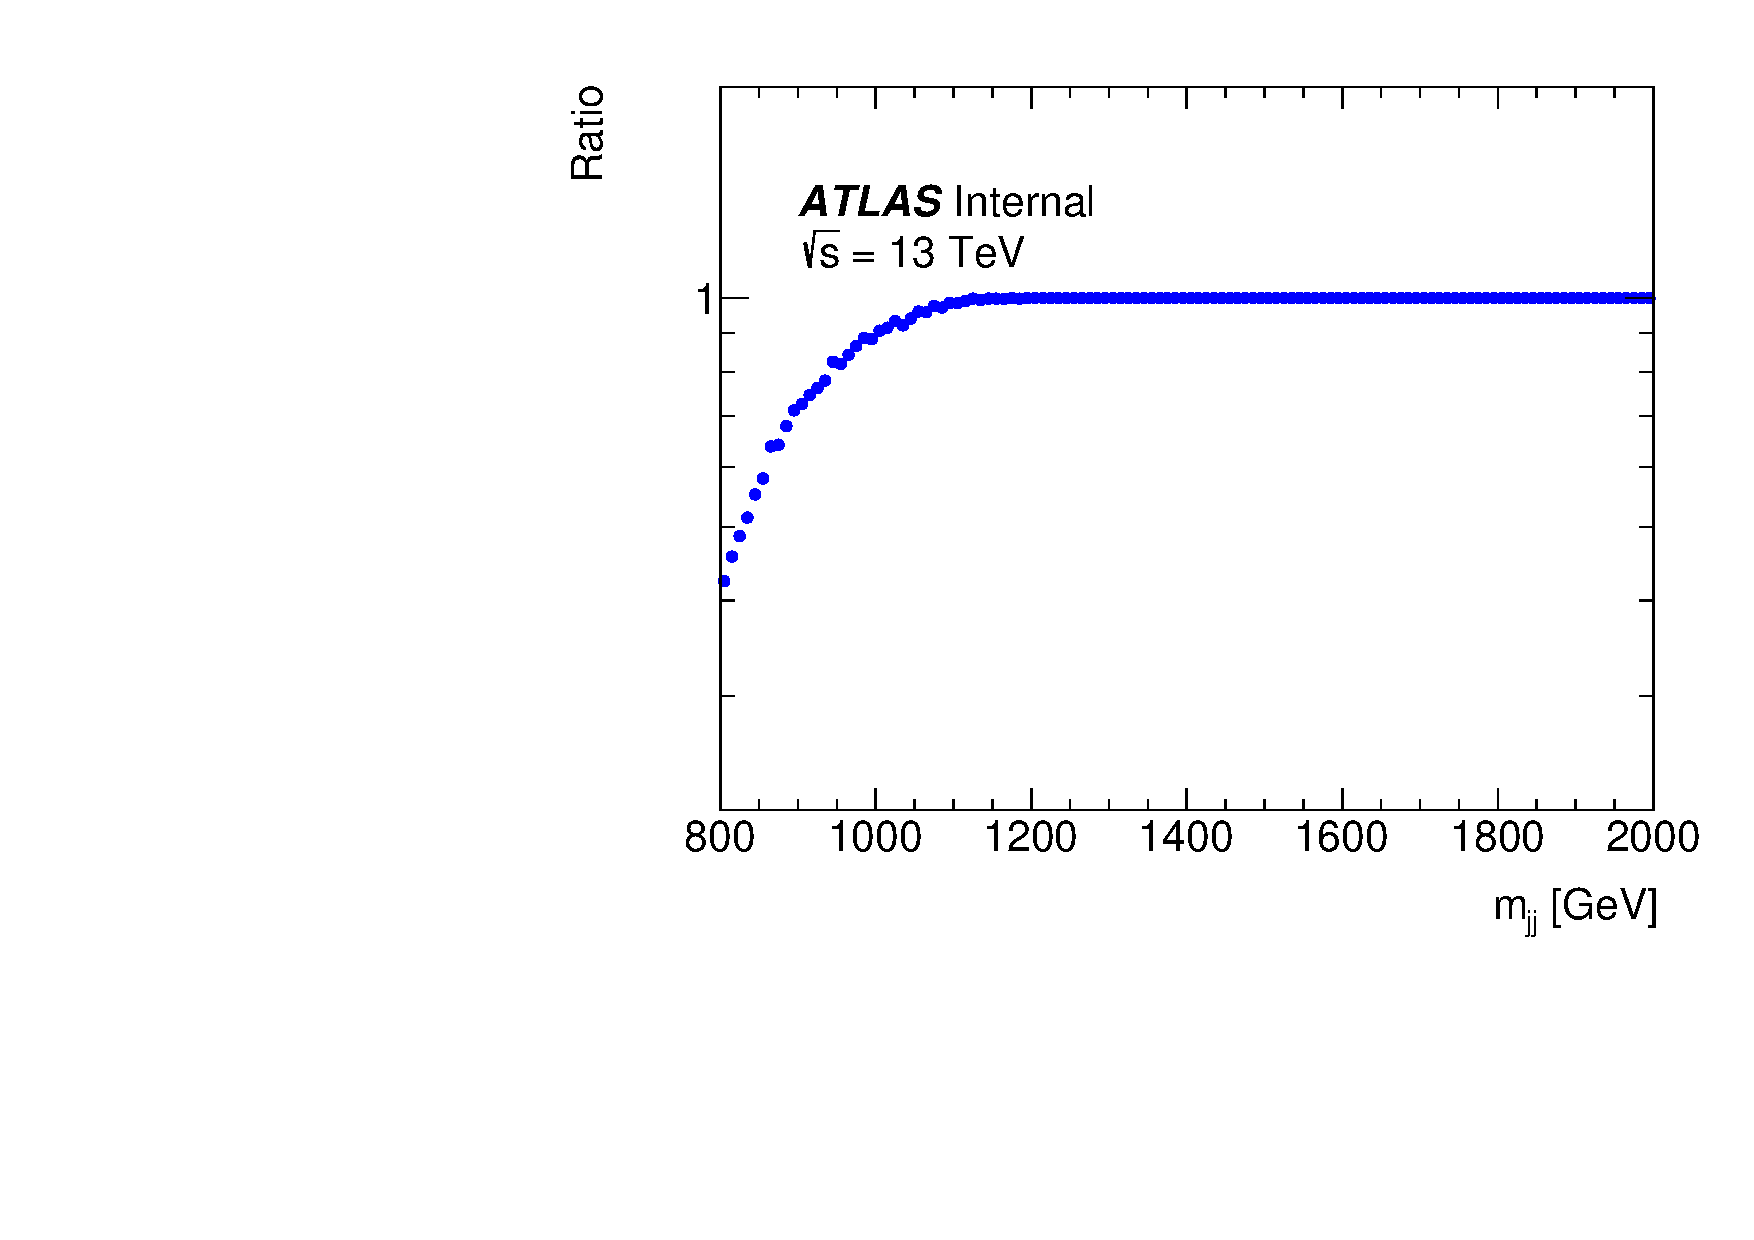
\includegraphics[width=0.48\columnwidth]{figures/massturnon/app_triggerturnon/Ratio_mjj_gg_turnon_yStar0p8_Data17}}

        \caption{Efficiencies as a function of \mjj\ for $|\ystar|<0.8$ using HLT\_j420 compared with HLT\_mu50 in the case of comparison of mass spectra with
        (a) $\geq$1 g-tag, (b) 2 g-tag and the ratio between the two (c) $\geq$1 g-tag and (d) 2 g-tag for 2017 data.}
\end{figure}

\begin{figure}[htbp]
        \centering
        \subfigure[$\geq$1 g-tag]{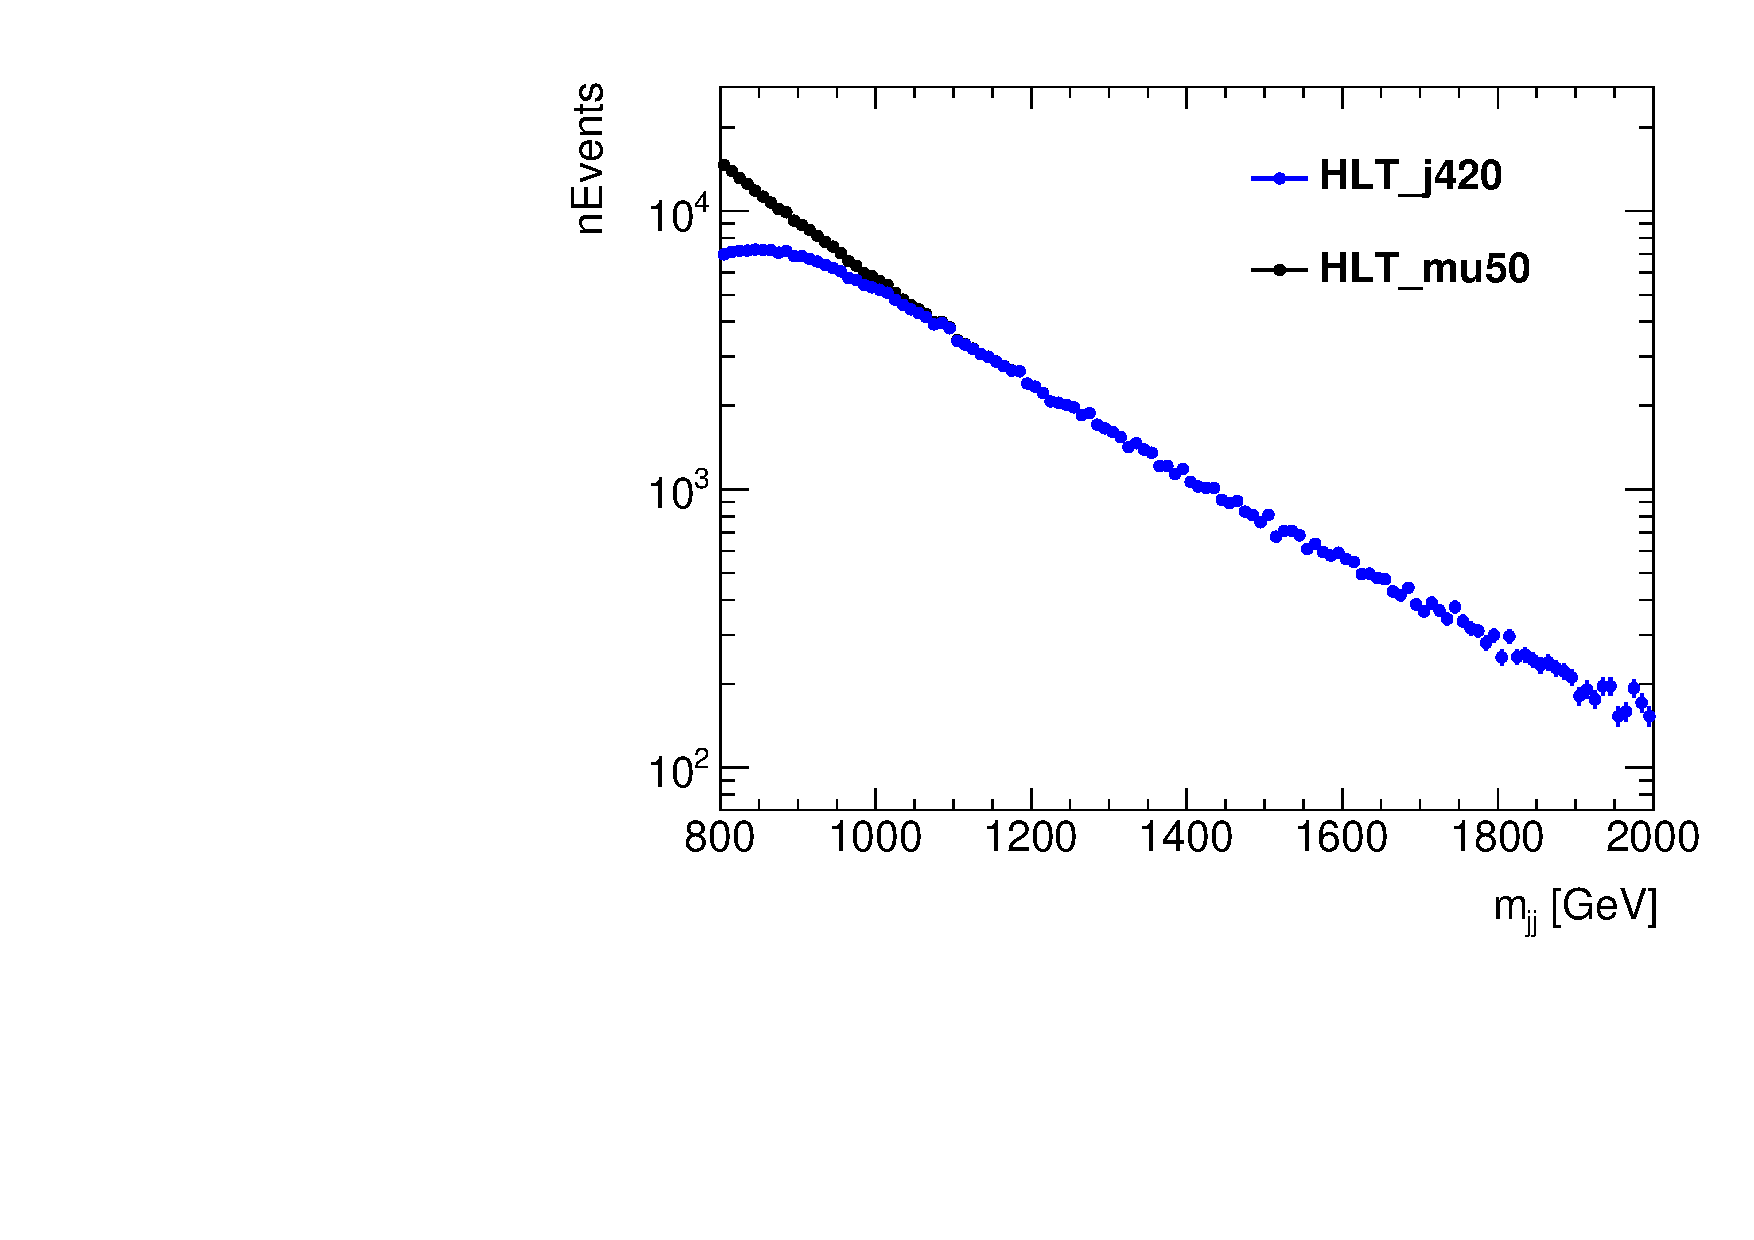
\includegraphics[width=0.48\columnwidth]{figures/massturnon/app_triggerturnon/mjj_qg_turnon_yStar0p8_Data18}}
        \subfigure[2 g-tag]{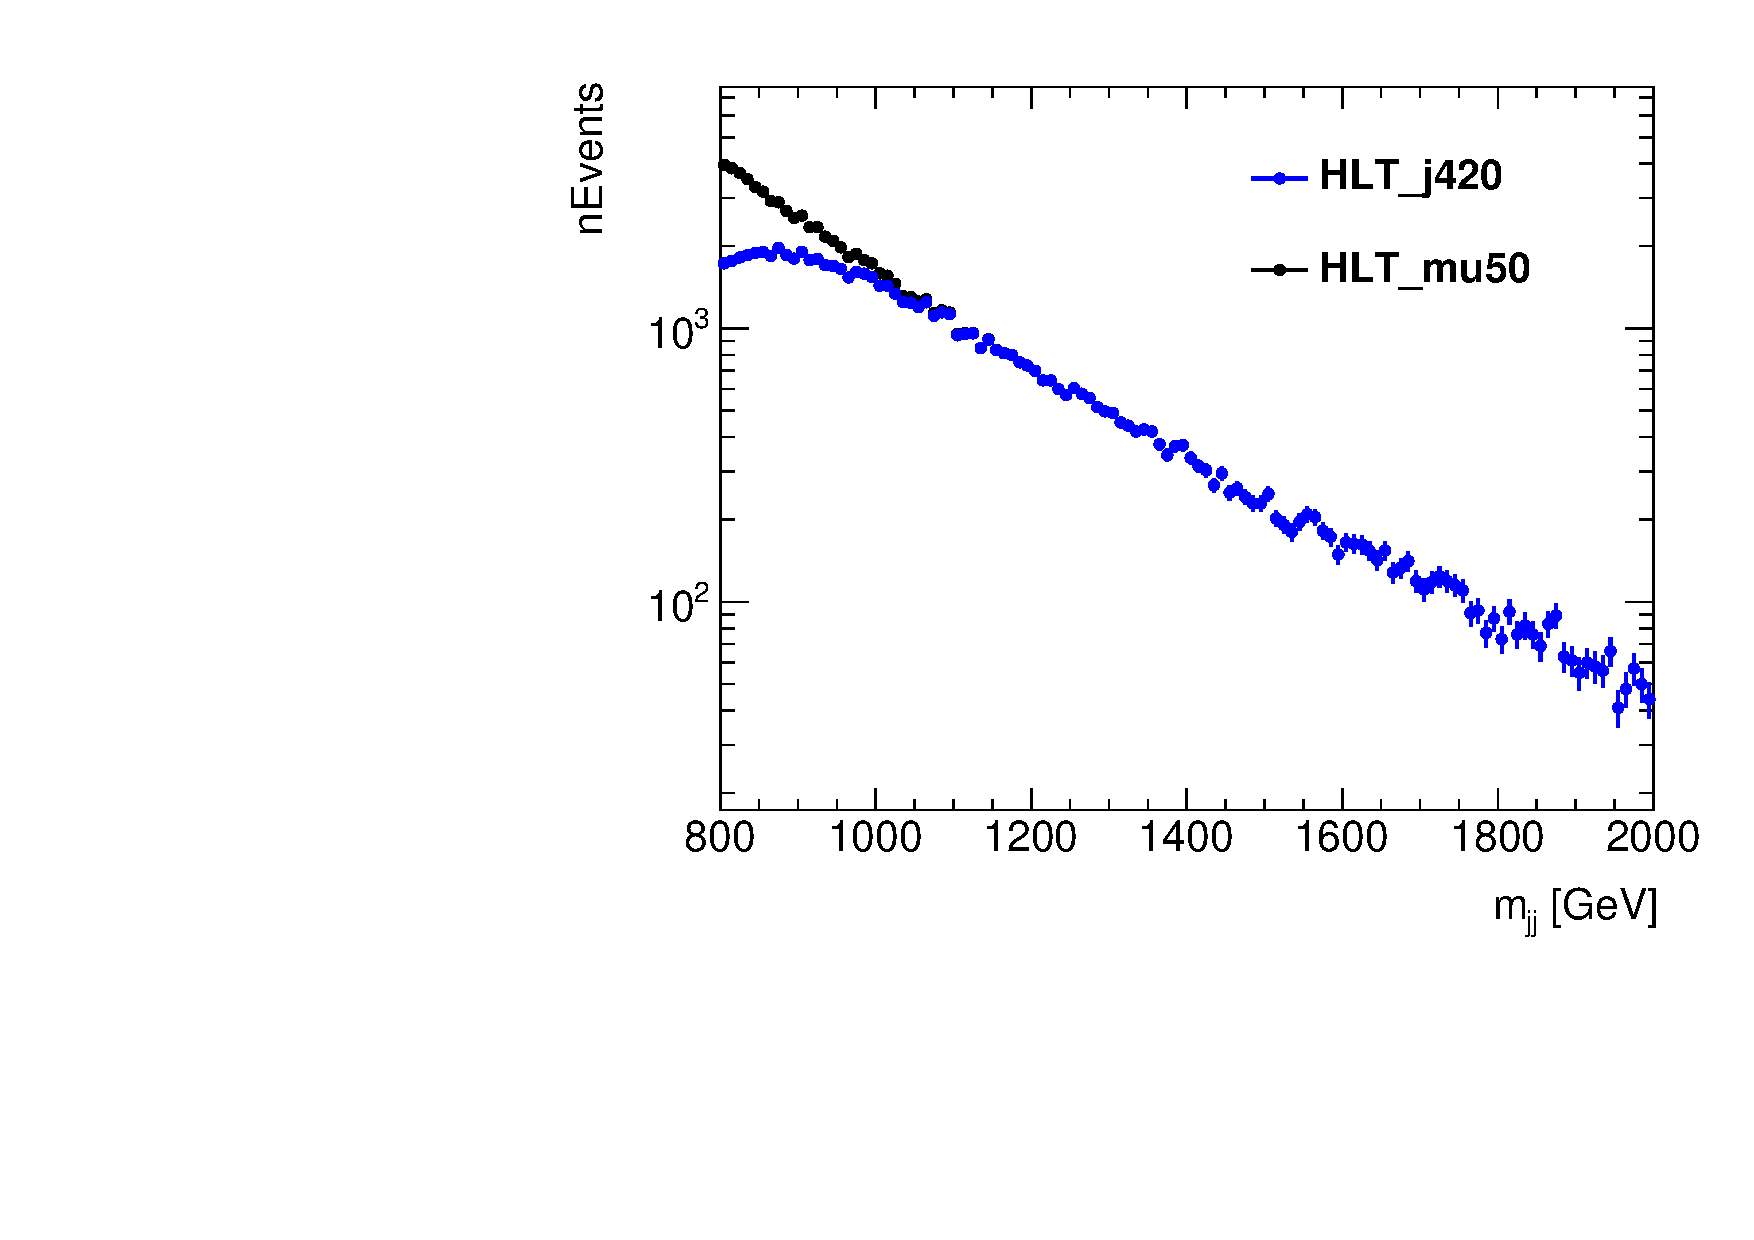
\includegraphics[width=0.48\columnwidth]{figures/massturnon/app_triggerturnon/mjj_gg_turnon_yStar0p8_Data18}}
        \\
        \subfigure[$\geq$1 g-tag]{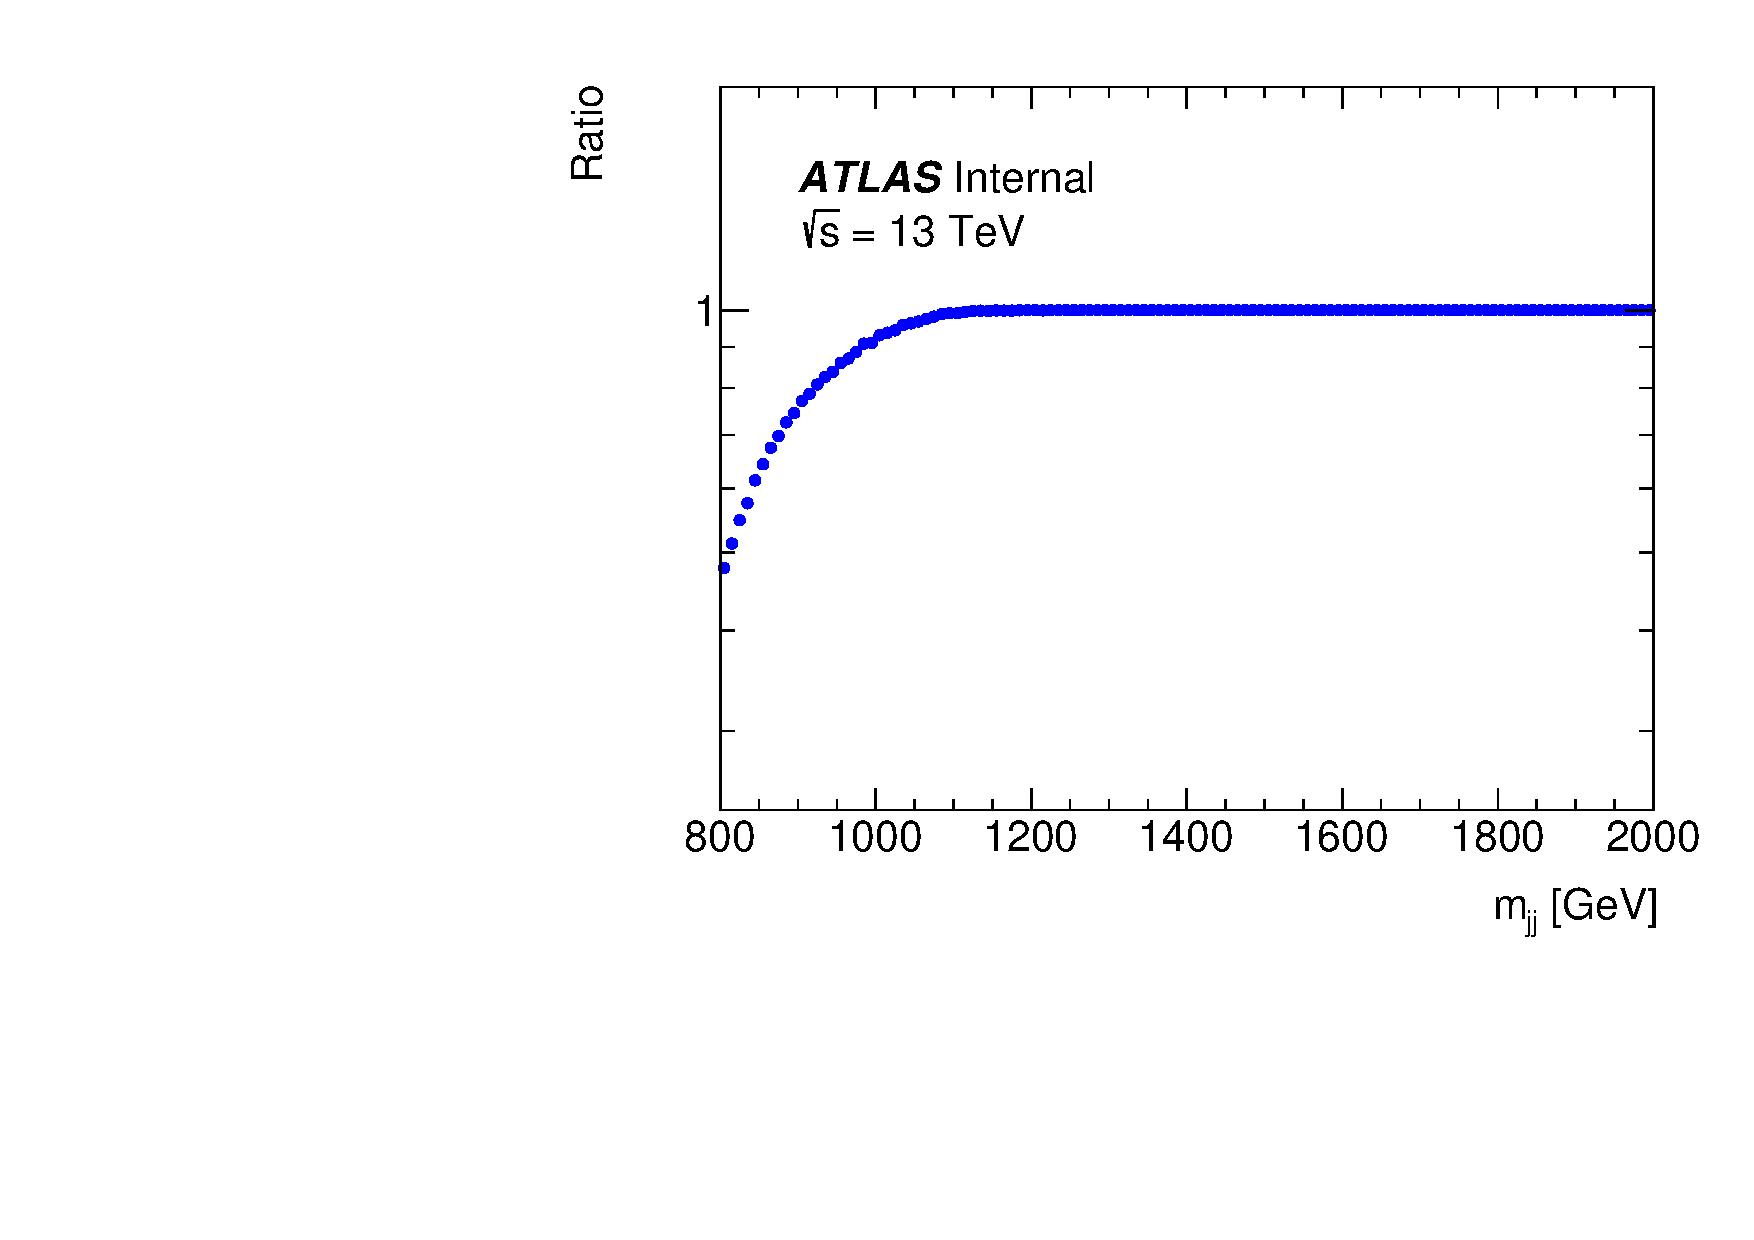
\includegraphics[width=0.48\columnwidth]{figures/massturnon/app_triggerturnon/Ratio_mjj_qg_turnon_yStar0p8_Data18}}
        \subfigure[2 g-tag]{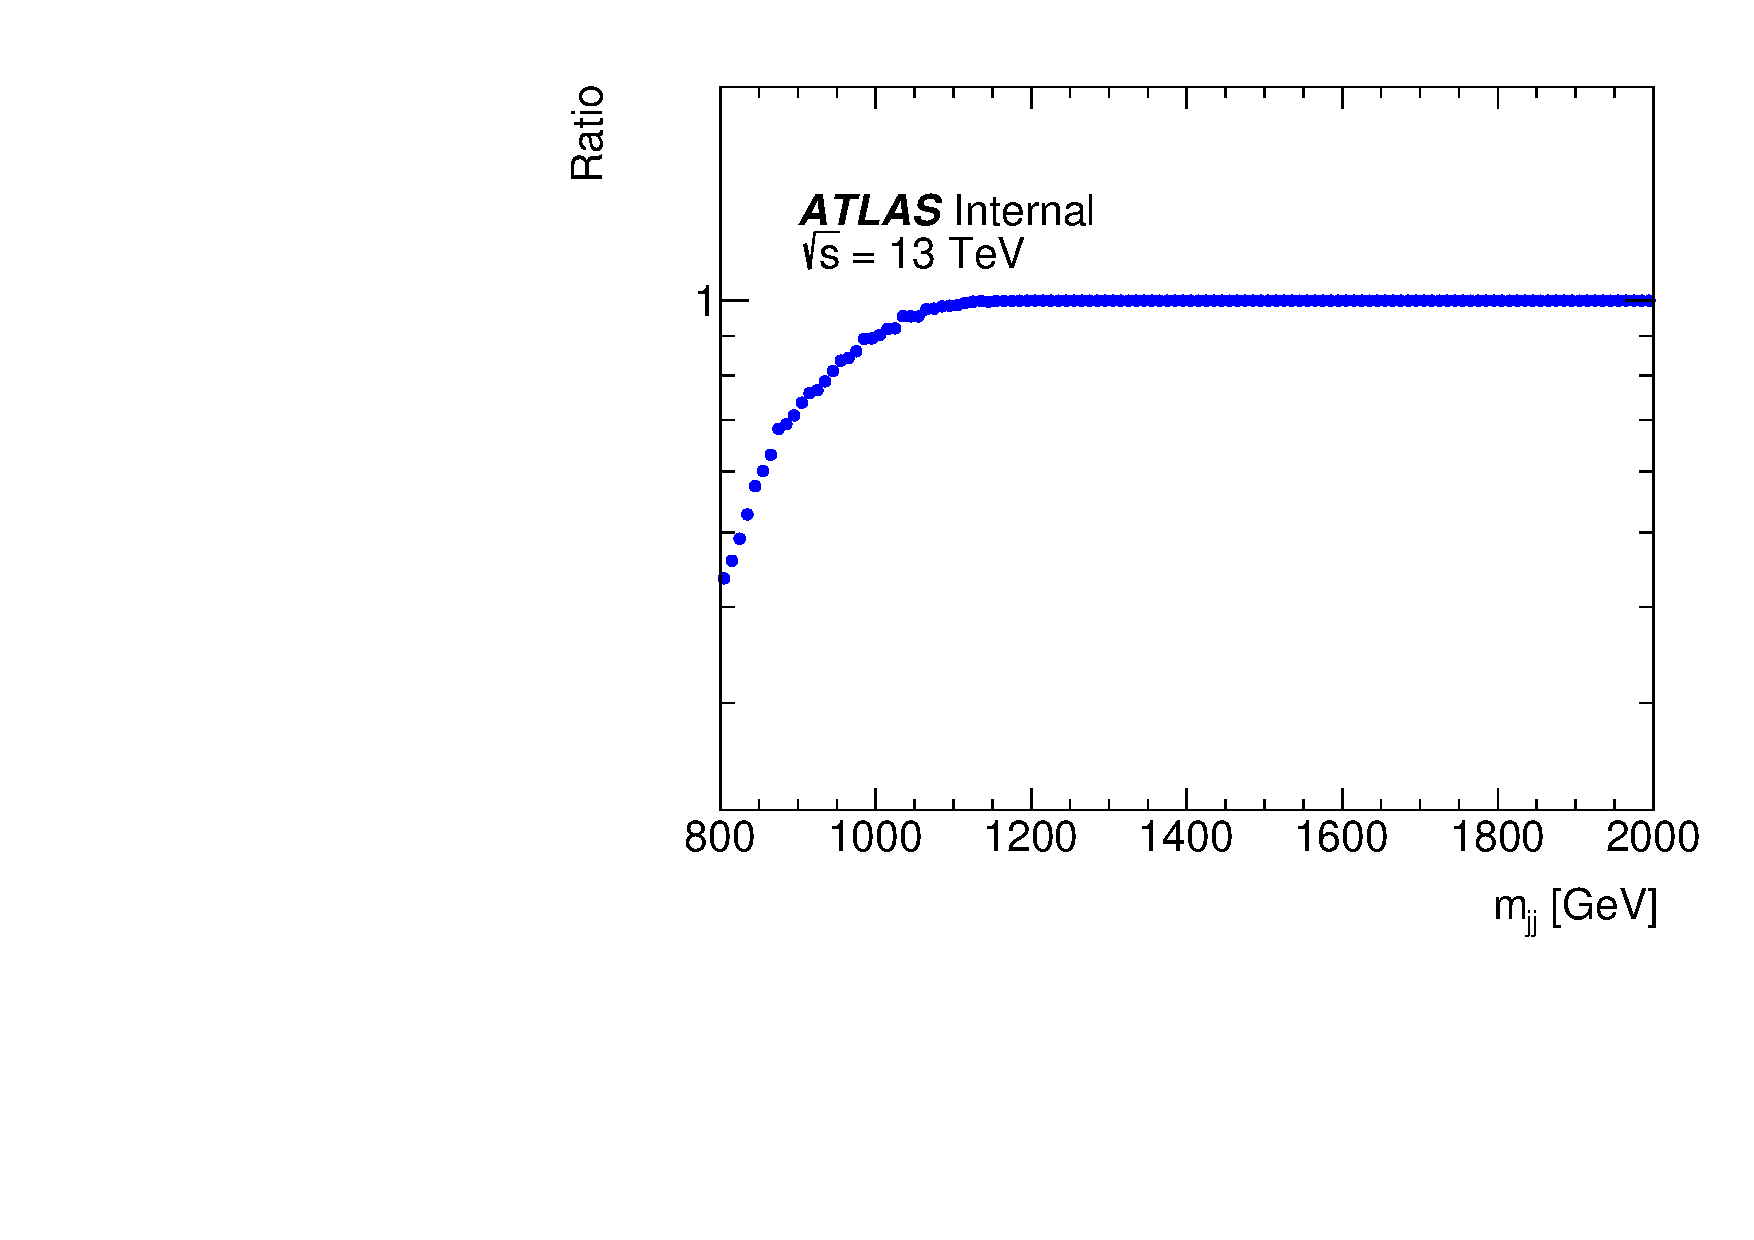
\includegraphics[width=0.48\columnwidth]{figures/massturnon/app_triggerturnon/Ratio_mjj_gg_turnon_yStar0p8_Data18}}

        \caption{Efficiencies as a function of \mjj\ for $|\ystar|<0.8$ using HLT\_j420 compared with HLT\_mu50 in the case of comparison of mass spectra with
        (a) $\geq$1 g-tag, (b) 2 g-tag and the ratio between the two (c) $\geq$1 g-tag and (d) 2 g-tag for 2018 data.}
        \label{fig:trigger-yStar0p8-Data18}
\end{figure}
